\documentclass[zihao=-4,UTF8,openany]{ctexart}

\usepackage[a4paper,left=2.5cm,right=2.5cm,top=2.8cm,bottom=2.5cm]{geometry}
\usepackage{amsmath,amssymb}
\usepackage{newunicodechar}
\newunicodechar{✓}{$\checkmark$}
\newunicodechar{✗}{$\times$}
\newunicodechar{∈}{$\in$}
\newunicodechar{▼}{$\blacktriangledown$}
\usepackage{graphicx}
\usepackage{booktabs}
\usepackage{longtable}
\usepackage{array}
\usepackage{calc}
\usepackage{float}
\usepackage{caption}
\usepackage{fancyhdr,needspace,enumitem,placeins}
\usepackage{xcolor}
\usepackage{listings}
\lstset{
  language=Java,
  basicstyle=\footnotesize\ttfamily,
  keywordstyle=\color{blue!60!black}\bfseries,
  commentstyle=\color{green!45!black},
  stringstyle=\color{red!60!black},
  numbers=left,
  numberstyle=\tiny\color{gray},
  numbersep=6pt,
  frame=single,
  rulecolor=\color{gray!40},
  breaklines=true,
  columns=fullflexible,
  keepspaces=true,
  showstringspaces=false,
  tabsize=4
}
\usepackage{tikz}
\usetikzlibrary{arrows.meta, positioning, shapes.geometric}
\usepackage[hidelinks]{hyperref}

\graphicspath{{media/}}

\setlength{\parindent}{2em}
\setlength{\parskip}{1pt}
\emergencystretch=2em
\captionsetup{font=small}

% 允许代码标识符在下划线处换行，减少越界
\renewcommand{\_}{\textunderscore\allowbreak}

\usepackage{etoolbox}
\AtBeginEnvironment{longtable}{\small}

\hypersetup{
  pdftitle={企业级 CMS 内容管理系统 · 课程设计报告},
  pdfauthor={孙贤泽、姚霖锋、潘凤乐、王储},
}

\setcounter{tocdepth}{2}
\raggedbottom
\setlist{itemsep=2pt,topsep=4pt,parsep=0pt}
\setlength{\headheight}{15pt}
\pagestyle{fancy}
\fancyhf{}
\fancyhead[L]{\small JAVA 框架技术（一）课程设计}
\fancyhead[R]{\small 云章 CMS 内容管理系统}
\fancyfoot[C]{\thepage}
\renewcommand{\headrulewidth}{0.4pt}
\ctexset{section={beforeskip=18pt,afterskip=10pt},subsection={beforeskip=12pt,afterskip=6pt},subsubsection={beforeskip=9pt,afterskip=4pt}}
\clubpenalty=10000
\widowpenalty=10000
\captionsetup{font=small,labelfont=bf,skip=5pt}
\lstset{basicstyle=\small\ttfamily,aboveskip=8pt,belowskip=8pt,xleftmargin=1em,framexleftmargin=0.4em}
\newcommand{\reportfigure}[4][0.94\linewidth]{%
  \begin{figure}[H]\centering
  \includegraphics[width=#1,height=0.48\textheight,keepaspectratio]{#2}
  \caption{#3}\label{#4}
  \end{figure}}

\begin{document}
\begin{titlepage}
\centering
\vspace*{1.8cm}

{\zihao{2}\heiti《JAVA 框架技术（一）》}\\[0.8cm]
{\zihao{1}\heiti 课~程~设~计~报~告}\\[1.4cm]
{\zihao{2}\heiti 企业级 CMS 内容管理系统}\\[0.6cm]
{\zihao{4}\heiti 基于 Spring Boot 与 MyBatis-Plus 的实现}\\[3.2cm]

{\zihao{4}\songti
\begin{tabular}{rl}
姓\quad 名： & 孙贤泽 \quad 姚霖锋 \quad 潘凤乐 \quad 王储 \\[1.1cm]
学\quad 号： & 20241923 \quad 20241891 \quad 20241922 \quad 20241925 \\[1.1cm]
班\quad 级： & \underline{\hspace{5.5cm}} \\[1.1cm]
指导教师： & \underline{\hspace{5.5cm}} \\
\end{tabular}}

\vfill
{\zihao{4}2026 年 11 月}
\end{titlepage}

\pagenumbering{Roman}
{\small\tableofcontents}
\clearpage
\pagenumbering{arabic}

\section*{摘要}\label{ux6458ux8981}
\addcontentsline{toc}{section}{摘要}

本项目面向内容发布与审核场景，设计并实现了云章 CMS 内容管理系统。系统采用 Spring Boot、MyBatis-Plus 和 Thymeleaf，提供用户与角色管理、多级分类、文章编辑与审核、组合检索、操作日志及前台阅读功能。数据库以用户、角色、权限、文章、分类和日志六类实体为基础，通过关联表维护授权关系。

系统使用接口权限校验和数据归属检查限制操作范围，以状态迁移表管理文章从草稿到发布、下架的过程，并通过统一异常处理和日志脱敏记录失败原因。列表查询通过关联取数减少逐条查询，站内引导模块通过页面卡片提供导航。项目已有测试记录覆盖状态迁移、权限边界和部分异常场景；并发性能和数据库集成测试仍需进一步补充。

\textbf{关键词：}内容管理系统；文章审核；权限控制；MyBatis-Plus；操作日志

\section*{一、项目概述}\label{ux4e00ux9879ux76eeux6982ux8ff0}
\addcontentsline{toc}{section}{一、项目概述}



\subsection*{1.1 背景与目标}\label{ux80ccux666fux4e0eux76eeux6807}
\addcontentsline{toc}{subsection}{1.1 背景与目标}

本项目以内容管理系统为对象，完成从用户登录、文章编写、提交审核到前台展示的完整业务流程。设计重点包括：为不同角色划分操作范围，保证文章按规定流程发布，维护分类与内容之间的关系，并记录关键操作以便排查问题。

系统名称为云章 CMS。管理端服务于作者、审核员和管理员，前台面向内容读者。报告按照需求、数据库、系统设计、功能实现、测试及部署的顺序说明项目。

\subsection*{1.2 系统功能概览}\label{ux6253ux5f00ux80fdux5e72ux4ec0ux4e48}
\addcontentsline{toc}{subsection}{1.2 系统功能概览}

系统分为管理端与前台两部分，管理端按角色动态显示菜单，逐页说明如下。

登录页用账号密码登录，失败时给出明确原因，区分密码错误与账号停用。工作台展示我的草稿、审核中、被驳回、已发布四张状态卡片，附带全站待审与已发布统计和最近稿件。文章列表支持关键词、分类含子分类、状态、作者、仅看我的组合筛选，配合多维排序与分页，并提供批量通过与批量下架。写文章页包含标题、摘要、正文与分类，可保存草稿或提交审核，保存前做敏感信息预检。内容审核页展示待审稿件，支持通过与驳回，驳回意见必填，且不能审核自己的稿件。分类管理以三级树展示，支持新增、改名、排序、启用停用与删除，存在子分类或文章引用时拒绝删除。用户管理负责用户的增删改查、启用停用与角色分配。角色与权限页维护角色并勾选权限点，采用全量覆盖式保存。操作日志页按类型、结果、操作人、时间筛选，查看脱敏后的入参与耗时。

前台阅读站展示已发布文章列表与详情，阅读量累加，支持按分类浏览。站内引导以右下角悬浮球形式，用自然语言提问即可返回可点击的页面卡片，并可跳转到对应页面。

\subsection*{1.3 规模与交付形态}\label{ux89c4ux6a21ux4e0eux4ea4ux4ed8ux5f62ux6001}
\addcontentsline{toc}{subsection}{1.3 规模与交付形态}

Java 源文件共 103 个、5 771 行，用 find 命令对 src/main/java 统计。前端模块 17 个、2 349 行，对应 static/js 下的脚本文件。Thymeleaf 模板 13 个。数据表 8 张，其中 6 张主表加 2 张关联表。REST 接口 49 个操作、37 条路径，由 apifox/cms-openapi.json 解析计数。单元测试 33 个、分属 6 个测试类，mvn -o test 全部通过。权限点 15 个、角色 4 个。引导卡片 9 张，启动日志显示 9 张卡片、0 个未覆盖 Controller。

\section*{二、需求分析}\label{ux4e8cux9700ux6c42ux5206ux6790}
\addcontentsline{toc}{section}{二、需求分析}



\subsection*{2.1 业务背景与用户画像}\label{ux4e1aux52a1ux80ccux666fux4e0eux7528ux6237ux753bux50cf}
\addcontentsline{toc}{subsection}{2.1 业务背景与用户画像}

系统围绕文章的编写、审核和阅读组织业务。作者需要保存和修改草稿，审核员需要确认内容是否适合发布，管理员负责账号、权限和分类维护，读者只查看已发布的文章。为避免未审核内容外发，编辑操作和发布操作需要区分权限；为防止误删，分类与文章之间的关联需要在删除时检查。

\subsection*{2.2 范围界定}\label{ux8303ux56f4ux754cux5b9a}
\addcontentsline{toc}{subsection}{2.2 范围界定}

本项目包含用户管理、权限管控、内容分类、文章发布、内容审核、数据检索、日志记录和站内引导智能体八个部分。

用户管理负责注册、登录、退出、启停和角色分配。权限管控做接口级与数据级双层校验，接口级用 AOP 注解，数据级按数据归属判断。内容分类实现三级树、增删改、启停、排序以及与文章的绑定。文章发布覆盖起草、编辑、提交、撤回、再提交和删除。内容审核支持通过、驳回、批量通过和上下架，驳回时必须填写意见。数据检索支持按关键词、分类、状态、作者组合筛选，分类自动包含子分类，并支持多维排序。日志记录覆盖所有写操作与登录，结果分为成功、被拦截、失败三类。站内引导智能体是附加模块，回答某个页面在哪、怎么用。

本项目不包含以下内容，明确划界，避免文档写得比代码多。

富文本编辑器、附件与图片上传不在范围内，属于课程要求之外，敏感信息防护因此只落在文章保存链路，不假装支持上传管控。站内全文搜索不引入倒排索引，用 LIKE 满足课程数据量，性能取舍写入已知边界。多租户、消息通知、自定义审批流属于平台化能力，与本次考核点无关。分类不支持更换上级，保持 level 冗余字段一致性的成本高于收益，采用删除后重建的方式。

\subsection*{2.3 角色定义}\label{ux89d2ux8272ux5b9aux4e49}
\addcontentsline{toc}{subsection}{2.3 角色定义}

系统分四个角色。游客编码 GUEST，只读浏览前台已发布文章，对应普通读者。作者编码 AUTHOR，撰写、修改自己的稿件并提交审核，对应编辑和记者。审核员编码 AUDITOR，负责审核稿件、发布与下架，对应内容主管。管理员编码 ADMIN，全面管理用户、角色、权限、分类与日志。

一个用户可拥有多个角色，最终权限是所属全部角色权限的并集。注册用户默认分配 AUTHOR（RoleCode.DEFAULT）。

\subsection*{2.4 权限点与权限矩阵}\label{ux6743ux9650ux70b9ux4e0eux6743ux9650ux77e9ux9635}
\addcontentsline{toc}{subsection}{2.4 权限点与权限矩阵}

权限点由初始化脚本写入，运行期只读，共 15 个：

\begin{longtable}[]{@{}
  >{\raggedright\arraybackslash}p{(\linewidth - 10\tabcolsep) * \real{0.2812}}
  >{\raggedright\arraybackslash}p{(\linewidth - 10\tabcolsep) * \real{0.2187}}
  >{\raggedright\arraybackslash}p{(\linewidth - 10\tabcolsep) * \real{0.1250}}
  >{\raggedright\arraybackslash}p{(\linewidth - 10\tabcolsep) * \real{0.1250}}
  >{\raggedright\arraybackslash}p{(\linewidth - 10\tabcolsep) * \real{0.1250}}
  >{\raggedright\arraybackslash}p{(\linewidth - 10\tabcolsep) * \real{0.1250}}@{}}
\toprule\noalign{}
\begin{minipage}[b]{\linewidth}\raggedright
\textbf{权限点}
\end{minipage} & \begin{minipage}[b]{\linewidth}\raggedright
\textbf{说明}
\end{minipage} & \begin{minipage}[b]{\linewidth}\raggedright
\textbf{游客}
\end{minipage} & \begin{minipage}[b]{\linewidth}\raggedright
\textbf{作者}
\end{minipage} & \begin{minipage}[b]{\linewidth}\raggedright
\textbf{审核员}
\end{minipage} & \begin{minipage}[b]{\linewidth}\raggedright
\textbf{管理员}
\end{minipage} \\
\midrule\noalign{}
\endhead
\bottomrule\noalign{}
\endlastfoot
article:read & 查看文章 & ✓ & ✓ & ✓ & ✓ \\
article:create & 新建文章 & ✗ & ✓ & ✗ & ✓ \\
article:update:own & 修改自己的文章 & ✗ & ✓ & ✗ & ✓ \\
article:update:any & 修改任意文章 & ✗ & ✗ & ✓ & ✓ \\
article:delete:own & 删除自己的文章 & ✗ & ✓ & ✗ & ✓ \\
article:delete:any & 删除任意文章 & ✗ & ✗ & ✗ & ✓ \\
article:submit & 提交审核 & ✗ & ✓ & ✗ & ✓ \\
article:audit & 审核文章 & ✗ & ✗ & ✓ & ✓ \\
article:publish & 发布与下架 & ✗ & ✗ & ✓ & ✓ \\
category:read & 查看分类 & ✓ & ✓ & ✓ & ✓ \\
category:write & 维护分类 & ✗ & ✗ & ✗ & ✓ \\
user:manage & 用户管理 & ✗ & ✗ & ✗ & ✓ \\
role:manage & 角色管理 & ✗ & ✗ & ✗ & ✓ \\
log:read & 查看操作日志 & ✗ & ✗ & ✗ & ✓ \\
guide:use & 使用站内引导 & ✓ & ✓ & ✓ & ✓ \\
\end{longtable}

矩阵中的"✓/✗"与 sql/data.sql 的 sys\_role\_permission 插入语句一一对应，不是凭印象填写。管理员用 SELECT 4, id FROM sys\_permission 全量授权，新增权限点无需改脚本。

\subsection*{2.5 核心业务场景}\label{ux6838ux5fc3ux4e1aux52a1ux573aux666f}
\addcontentsline{toc}{subsection}{2.5 核心业务场景}

以下七个场景是本次设计的验收范围。

第一个场景是文章发布，参与者是作者。作者输入标题、摘要、正文和所属分类，起草后保存为草稿，反复修改到满意再提交审核。输出是一篇进入待审队列的稿件。价值在于稿子先落草稿、改好才提交，半成品不会漏给读者，写和发之间多了一道边界。

第二个场景是分类管理，参与者是管理员。管理员输入分类名称、上级位置、排序和启停状态，新增根分类、挂子分类、调整排序、停用或删除。输出是一棵有序的分类树。价值在于内容有了清晰的归置，读者按分类就能找到想看的内容，不用在杂乱列表里翻找。

第三个场景是内容审核，参与者是审核员。审核员输入待审稿件并通读全文，判定后要么通过发布，要么驳回并填写意见。输出是上线可见的文章，或退回作者修改的稿件。价值在于一个人不能既写稿又审稿，敏感内容多一道把关，降低出错外发的风险。

第四个场景是用户管理，参与者是游客和管理员。游客输入用户名、密码、昵称、邮箱自助注册，再登录、退出；管理员新增、修改、停用、删除账号并分配角色。输出是一套账号体系，每个账号都带着明确角色。价值在于谁在操作系统一清二楚，人员离职时账号能及时停用回收。

第五个场景是权限管控，参与者是全部角色。一次操作进来，系统依次判断有没有登录、角色有没有对应权限、动的是不是自己的数据，满足才放行，否则拒绝并留痕。输出是允许执行或拒绝。价值在于作者改不了别人的稿，普通账号进不了管理功能，越权一律被拦下，数据不会被篡改。

第六个场景是数据检索，参与者是登录用户。用户输入关键词、分类、状态、作者等条件，再选排序方式和页码，组合筛选后分页翻看。输出是一页符合条件的结果。价值在于海量内容里几秒定位到想要的一篇，不用一页页翻，检索效率是内容系统的命脉。

第七个场景是日志记录，由系统自动完成。每次写操作，系统记录操作人、动作、对象、脱敏后的参数、结果和耗时。输出是一条可查询的操作流水。价值在于出了问题能追溯到谁在什么时间做了什么，越权尝试也有据可查，既缩短排查时间，也形成威慑。

\subsection*{2.6 业务规则与状态模型}\label{ux4e1aux52a1ux89c4ux5219ux4e0eux72b6ux6001ux6a21ux578b}
\addcontentsline{toc}{subsection}{2.6 业务规则与状态模型}

文章共五个状态，七条合法迁移。

作者提交审核，从 DRAFT 迁到 PENDING。作者撤回，从 PENDING 回到 DRAFT。审核通过，从 PENDING 迁到 PUBLISHED。驳回时意见必填，从 PENDING 迁到 REJECTED。按意见修改后再写，从 REJECTED 回到 DRAFT。下架时原因必填，从 PUBLISHED 迁到 OFFLINE。重新提交审核，从 OFFLINE 回到 PENDING。

表外迁移一律返回 409/40901。删除是状态机之外的独立规则：只有 DRAFT 与 REJECTED 可删。

\subsection*{2.7 非功能需求}\label{ux975eux529fux80fdux9700ux6c42}
\addcontentsline{toc}{subsection}{2.7 非功能需求}

安全上，密码用 BCrypt 不可逆存储，通过排序白名单加 \#\{\} 预编译防 SQL 注入，双层权限防越权，敏感信息检测加日志打码防外泄。性能上，列表页不得出现 N+1，用三表 join 解决，分页插件限制单页最多 200 条。可维护性上，分层清晰、职责单一，四个业务模块配合 ModuleBoundaryTest 检查边界。可运维性上，异常有统一出口，行为可追溯，对应 GlobalExceptionHandler、LogAspect 与 traceId。兼容性上，中文与 emoji 不截断，采用 utf8mb4。

\subsection*{2.8 需求跟踪矩阵（节选）}\label{ux9700ux6c42ux8ddfux8e2aux77e9ux9635ux8282ux9009}
\addcontentsline{toc}{subsection}{2.8 需求跟踪矩阵（节选）}

注册、登录、退出由 AuthService 实现，接口在 /api/auth 下，实机联调验证。角色分配由 UserService 实现，接口是 PUT /api/users/\{id\}/roles，实机联调验证。接口级权限由 PermissionAspect 实现，覆盖所有受控接口，越权返回 40300。数据级权限由 checkOwner 实现，用于文章改删，越权返回 40301。三级分类由 CategoryService 实现，接口在 /api/categories 下，四级分类被拒返回 40001。文章状态机由 ArticleStateMachine 实现，接口在 /api/articles/\{id\} 下，单测 4 个用例。多维检索由 ArticleMapper.selectPageVO 实现，接口是 GET /api/articles，用 SQL 条数核对。操作日志由 LogAspect 实现，日志页可见 DENIED 记录。敏感信息拦截由 SensitiveInfoDetector 实现，接口是 POST /api/articles/sensitive-check，单测 9 个用例加浏览器实测。

\section*{三、技术选型与依据}\label{ux4e09ux6280ux672fux9009ux578bux4e0eux4f9dux636e}
\addcontentsline{toc}{section}{三、技术选型与依据}

项目以 Java 11 为运行基准，使用 Spring Boot 2.7.18 组织应用配置，Spring MVC 处理页面与接口请求，MyBatis-Plus 3.5.3.1 完成数据访问。该组合与原有 SSM 实验衔接，便于在已有业务代码上增加权限校验、分页和统一异常处理。

持久层保留 Mapper 与 XML：常规增删改查使用 MyBatis-Plus，文章列表等关联查询使用 XML 显式描述取数关系和筛选条件，便于检查所需字段和查询过程。

前端采用 Thymeleaf 与原生 JavaScript 模块。页面由服务端渲染，筛选、弹窗和提交操作通过接口完成。当前方式便于课程项目部署，后续页面增加时仍需加强组件复用和前端测试。

数据库设计面向 MySQL 8，使用 InnoDB 和 utf8mb4；原项目联调记录使用 MariaDB 10.6.23。部署环境与联调环境分别说明，避免将兼容性假设作为已验证结果。

身份认证使用 Session，权限检查由拦截器、AOP 和业务层共同完成。密码处理使用 spring-security-crypto 中的 BCryptPasswordEncoder；本项目未接入整套 Spring Security，鉴权流程由项目自身维护。

接口使用 OpenAPI 3.0 描述，并通过 Apifox 联调。现有方案手工维护接口文档，因此接口修改后需要同步核对路径、参数和响应结构。

\section*{四、数据库架构设计}\label{ux56dbux6570ux636eux5e93ux67b6ux6784ux8bbeux8ba1}
\addcontentsline{toc}{section}{四、数据库架构设计}

数据库需要同时支持账号授权、文章审核和操作追踪。用户、角色与权限负责回答“谁可以执行什么操作”；文章与分类负责组织内容；日志记录关键操作及其结果。项目因此设置六张实体表，并增加两张关联表维护用户与角色、角色与权限的多对多关系，共八张表。

例如，一名用户可以兼任作者和审核员，一个角色也可以分配给多名用户，因此使用关联表保存授权关系。文章分别记录分类和作者，用于按分类检索和检查修改权限。日志保留操作人的可读信息，以便账号变动后仍能理解历史操作。

\subsection*{4.1 sys\_user 用户表}\label{sys_user-ux7528ux6237ux8868}
\addcontentsline{toc}{subsection}{4.1 sys\_user 用户表}

\begin{longtable}[]{@{}
  >{\raggedright\arraybackslash}p{(\linewidth - 6\tabcolsep) * \real{0.2358}}
  >{\raggedright\arraybackslash}p{(\linewidth - 6\tabcolsep) * \real{0.2453}}
  >{\raggedright\arraybackslash}p{(\linewidth - 6\tabcolsep) * \real{0.3113}}
  >{\raggedright\arraybackslash}p{(\linewidth - 6\tabcolsep) * \real{0.2076}}@{}}
\toprule\noalign{}
\begin{minipage}[b]{\linewidth}\raggedright
\textbf{字段}
\end{minipage} & \begin{minipage}[b]{\linewidth}\raggedright
\textbf{类型}
\end{minipage} & \begin{minipage}[b]{\linewidth}\raggedright
\textbf{约束}
\end{minipage} & \begin{minipage}[b]{\linewidth}\raggedright
\textbf{说明}
\end{minipage} \\
\midrule\noalign{}
\endhead
\bottomrule\noalign{}
\endlastfoot
id & BIGINT & PK, AUTO\_INCREMENT & 主键 \\
username & VARCHAR(50) & NOT NULL, UK uk\_user\_username & 登录名，创建后不可修改 \\
password & VARCHAR(100) & NOT NULL & BCrypt 密文 \\
nickname & VARCHAR(50) & NOT NULL DEFAULT \textquotesingle\textquotesingle{} & 展示名 \\
email / phone & VARCHAR(100) / VARCHAR(20) & DEFAULT NULL & 联系方式 \\
status & TINYINT & NOT NULL DEFAULT 1 & 1 启用 / 0 停用 \\
deleted & TINYINT & NOT NULL DEFAULT 0 & 逻辑删除 \\
create\_time / update\_time & DATETIME & NOT NULL, 默认当前时间 / 自动更新 & 审计字段 \\
create\_by / update\_by & BIGINT & DEFAULT NULL & 操作人 \\
\end{longtable}

用户表保存登录账号和基本资料。username 设置唯一约束，用于防止重复注册；id 作为其他表引用用户的标识。status 表示账号是否启用，deleted 表示是否逻辑删除，两者分别对应停用和删除操作。密码字段保存 BCrypt 处理后的结果，不保存明文密码。创建、更新时间及操作人字段用于追踪记录变更。

\subsection*{4.2 sys\_role 角色表}\label{sys_role-ux89d2ux8272ux8868}
\addcontentsline{toc}{subsection}{4.2 sys\_role 角色表}

\begin{longtable}[]{@{}
  >{\raggedright\arraybackslash}p{(\linewidth - 6\tabcolsep) * \real{0.2337}}
  >{\raggedright\arraybackslash}p{(\linewidth - 6\tabcolsep) * \real{0.1559}}
  >{\raggedright\arraybackslash}p{(\linewidth - 6\tabcolsep) * \real{0.3247}}
  >{\raggedright\arraybackslash}p{(\linewidth - 6\tabcolsep) * \real{0.2857}}@{}}
\toprule\noalign{}
\begin{minipage}[b]{\linewidth}\raggedright
\textbf{字段}
\end{minipage} & \begin{minipage}[b]{\linewidth}\raggedright
\textbf{类型}
\end{minipage} & \begin{minipage}[b]{\linewidth}\raggedright
\textbf{约束}
\end{minipage} & \begin{minipage}[b]{\linewidth}\raggedright
\textbf{说明}
\end{minipage} \\
\midrule\noalign{}
\endhead
\bottomrule\noalign{}
\endlastfoot
id & BIGINT & PK & 主键 \\
role\_code & VARCHAR(50) & NOT NULL, UK uk\_role\_code & 角色编码，代码常量为准 \\
role\_name & VARCHAR(50) & NOT NULL & 展示名 \\
description & VARCHAR(200) & DEFAULT NULL & 描述 \\
sort & INT & NOT NULL DEFAULT 100 & 展示顺序 \\
status & TINYINT & NOT NULL DEFAULT 1 & 启停 \\
deleted 等审计字段 & --- & 同上 & --- \\
\end{longtable}

角色表把权限组合成可以分配给用户的集合，例如作者和审核员具有不同的操作范围。role\_code 用于程序识别角色，role\_name 用于界面展示，调整名称不需要改变权限判断。sort 控制显示顺序，status 控制角色的启停。

\subsection*{4.3 sys\_permission 权限点表}\label{sys_permission-ux6743ux9650ux70b9ux8868}
\addcontentsline{toc}{subsection}{4.3 sys\_permission 权限点表}

\begin{longtable}[]{@{}
  >{\raggedright\arraybackslash}p{(\linewidth - 6\tabcolsep) * \real{0.1196}}
  >{\raggedright\arraybackslash}p{(\linewidth - 6\tabcolsep) * \real{0.1304}}
  >{\raggedright\arraybackslash}p{(\linewidth - 6\tabcolsep) * \real{0.2717}}
  >{\raggedright\arraybackslash}p{(\linewidth - 6\tabcolsep) * \real{0.4782}}@{}}
\toprule\noalign{}
\begin{minipage}[b]{\linewidth}\raggedright
\textbf{字段}
\end{minipage} & \begin{minipage}[b]{\linewidth}\raggedright
\textbf{类型}
\end{minipage} & \begin{minipage}[b]{\linewidth}\raggedright
\textbf{约束}
\end{minipage} & \begin{minipage}[b]{\linewidth}\raggedright
\textbf{说明}
\end{minipage} \\
\midrule\noalign{}
\endhead
\bottomrule\noalign{}
\endlastfoot
id & BIGINT & PK & 主键 \\
perm\_code & VARCHAR(64) & NOT NULL, UK uk\_perm\_code & 如 article:audit \\
perm\_name & VARCHAR(64) & NOT NULL & 展示名 \\
perm\_group & VARCHAR(32) & NOT NULL DEFAULT \textquotesingle\textquotesingle{} & 分组：内容 / 审核 / 分类 / 账号与权限 / 系统 \\
description & VARCHAR(200) & DEFAULT NULL & 说明 \\
sort & INT & NOT NULL DEFAULT 100 & 组内排序 \\
\end{longtable}

权限点表示一项明确的操作能力，例如审核文章或管理用户。perm\_code 唯一，供权限注解和角色授权使用；perm\_name 与 perm\_group 用于管理页面展示和分组。权限点由初始化脚本维护，角色通过关联表获得权限，避免在每个用户记录上重复存储权限列表。

\subsection*{4.4 cms\_category 分类表}\label{cms_category-ux5206ux7c7bux8868}
\addcontentsline{toc}{subsection}{4.4 cms\_category 分类表}

\begin{longtable}[]{@{}
  >{\raggedright\arraybackslash}p{(\linewidth - 6\tabcolsep) * \real{0.2536}}
  >{\raggedright\arraybackslash}p{(\linewidth - 6\tabcolsep) * \real{0.1690}}
  >{\raggedright\arraybackslash}p{(\linewidth - 6\tabcolsep) * \real{0.2817}}
  >{\raggedright\arraybackslash}p{(\linewidth - 6\tabcolsep) * \real{0.2958}}@{}}
\toprule\noalign{}
\begin{minipage}[b]{\linewidth}\raggedright
\textbf{字段}
\end{minipage} & \begin{minipage}[b]{\linewidth}\raggedright
\textbf{类型}
\end{minipage} & \begin{minipage}[b]{\linewidth}\raggedright
\textbf{约束}
\end{minipage} & \begin{minipage}[b]{\linewidth}\raggedright
\textbf{说明}
\end{minipage} \\
\midrule\noalign{}
\endhead
\bottomrule\noalign{}
\endlastfoot
id & BIGINT & PK & 主键 \\
parent\_id & BIGINT & NOT NULL DEFAULT 0 & 上级分类，0 表示根 \\
name & VARCHAR(50) & NOT NULL & 分类名 \\
level & TINYINT & NOT NULL DEFAULT 1 & 层级 1--3，服务端推导 \\
sort & INT & NOT NULL DEFAULT 100 & 同级排序 \\
status & TINYINT & NOT NULL DEFAULT 1 & 启停 \\
description & VARCHAR(200) & DEFAULT NULL & 描述 \\
deleted 等审计字段 & --- & 同上 & --- \\
\end{longtable}

分类通过 parent\_id 表示上下级关系，根分类使用 0，层级由服务端根据父节点计算，最多三级。同一父分类下的名称通过 parent\_id 与 name 的组合唯一约束限制，sort 用于调整同级显示顺序。

当前设计没有为 parent\_id 建立自引用外键，父节点存在性和层级合法性由服务层检查。分类编辑不允许更换上级；删除前检查是否仍有子分类或文章引用，避免删除父分类后留下无法定位的子分类，或使文章失去有效分类。

\subsection*{4.5 cms\_article 文章表}\label{cms_article-ux6587ux7ae0ux8868}
\addcontentsline{toc}{subsection}{4.5 cms\_article 文章表}

\begin{longtable}[]{@{}
  >{\raggedright\arraybackslash}p{(\linewidth - 6\tabcolsep) * \real{0.4021}}
  >{\raggedright\arraybackslash}p{(\linewidth - 6\tabcolsep) * \real{0.1237}}
  >{\raggedright\arraybackslash}p{(\linewidth - 6\tabcolsep) * \real{0.3299}}
  >{\raggedright\arraybackslash}p{(\linewidth - 6\tabcolsep) * \real{0.1443}}@{}}
\toprule\noalign{}
\begin{minipage}[b]{\linewidth}\raggedright
\textbf{字段}
\end{minipage} & \begin{minipage}[b]{\linewidth}\raggedright
\textbf{类型}
\end{minipage} & \begin{minipage}[b]{\linewidth}\raggedright
\textbf{约束}
\end{minipage} & \begin{minipage}[b]{\linewidth}\raggedright
\textbf{说明}
\end{minipage} \\
\midrule\noalign{}
\endhead
\bottomrule\noalign{}
\endlastfoot
id & BIGINT & PK & 主键 \\
title & VARCHAR(200) & NOT NULL & 标题 \\
summary & VARCHAR(500) & DEFAULT NULL & 摘要 \\
content & MEDIUMTEXT & NOT NULL & 正文纯文本 \\
category\_id & BIGINT & NOT NULL, FK fk\_article\_category & 所属分类 \\
author\_id & BIGINT & NOT NULL, FK fk\_article\_author & 作者 \\
status & VARCHAR(16) & NOT NULL DEFAULT \textquotesingle DRAFT\textquotesingle{} & 五态之一 \\
auditor\_id & BIGINT & DEFAULT NULL & 最后审核人 \\
audit\_opinion & VARCHAR(500) & DEFAULT NULL & 审核意见 \\
audit\_time / submit\_time / publish\_time & DATETIME & DEFAULT NULL & 三个关键时间点 \\
offline\_reason & VARCHAR(500) & DEFAULT NULL & 下架原因 \\
view\_count & INT & NOT NULL DEFAULT 0 & 阅读量 \\
version & INT & NOT NULL DEFAULT 0 & 乐观锁版本号 \\
deleted 等审计字段 & --- & 同上 & --- \\
\end{longtable}

\begin{longtable}[]{@{}
  >{\raggedright\arraybackslash}p{(\linewidth - 2\tabcolsep) * \real{0.6296}}
  >{\raggedright\arraybackslash}p{(\linewidth - 2\tabcolsep) * \real{0.3704}}@{}}
\toprule\noalign{}
\begin{minipage}[b]{\linewidth}\raggedright
\textbf{索引}
\end{minipage} & \begin{minipage}[b]{\linewidth}\raggedright
\textbf{覆盖的查询}
\end{minipage} \\
\midrule\noalign{}
\endhead
\bottomrule\noalign{}
\endlastfoot
idx\_article\_query(status, category\_id, create\_time) & 列表页"状态 + 分类 + 时间倒序" \\
idx\_article\_author(author\_id, status) & "我的稿件"与按作者统计 \\
idx\_article\_title(title) & 标题前缀匹配 \\
idx\_article\_publish(publish\_time) & 前台按发布时间倒序 \\
\end{longtable}

文章通过 category\_id 关联分类，通过 author\_id 关联作者，两列设置外键，约束引用对象的存在性。auditor\_id 记录最后审核人，采用弱引用；审核时间、意见和发布时间记录相应业务节点。

status 保存草稿、待审核、已发布、被驳回、已下架五种状态，允许的迁移由业务层统一控制。version 用于检测编辑时的版本冲突。列表相关索引按分类、状态、作者及时间等查询条件设置，实际使用效果需要结合执行计划验证。

\subsection*{4.6 sys\_log 操作日志表}\label{sys_log-ux64cdux4f5cux65e5ux5fd7ux8868}
\addcontentsline{toc}{subsection}{4.6 sys\_log 操作日志表}

\begin{longtable}[]{@{}
  >{\raggedright\arraybackslash}p{(\linewidth - 6\tabcolsep) * \real{0.1491}}
  >{\raggedright\arraybackslash}p{(\linewidth - 6\tabcolsep) * \real{0.2281}}
  >{\raggedright\arraybackslash}p{(\linewidth - 6\tabcolsep) * \real{0.1053}}
  >{\raggedright\arraybackslash}p{(\linewidth - 6\tabcolsep) * \real{0.5175}}@{}}
\toprule\noalign{}
\begin{minipage}[b]{\linewidth}\raggedright
\textbf{字段}
\end{minipage} & \begin{minipage}[b]{\linewidth}\raggedright
\textbf{类型}
\end{minipage} & \begin{minipage}[b]{\linewidth}\raggedright
\textbf{约束}
\end{minipage} & \begin{minipage}[b]{\linewidth}\raggedright
\textbf{说明}
\end{minipage} \\
\midrule\noalign{}
\endhead
\bottomrule\noalign{}
\endlastfoot
id & BIGINT & PK & 主键 \\
user\_id & BIGINT & DEFAULT NULL & 操作人，弱引用 \\
username & VARCHAR(50) & DEFAULT NULL & 冗余用户名，便于人员删除后追溯 \\
log\_type & VARCHAR(20) & NOT NULL & LOGIN / ARTICLE / AUDIT / CATEGORY / USER / ROLE / AI\_QUERY \\
operation & VARCHAR(100) & NOT NULL & 可读操作名 \\
method & VARCHAR(200) & DEFAULT NULL & 类名\#方法名 \\
uri / http\_method & VARCHAR(200) / VARCHAR(10) & DEFAULT NULL & 请求信息 \\
params & VARCHAR(2000) & DEFAULT NULL & 脱敏后入参 \\
ip & VARCHAR(64) & DEFAULT NULL & 来源 IP \\
result & VARCHAR(20) & NOT NULL & SUCCESS / DENIED / FAIL \\
error\_msg & VARCHAR(400) & DEFAULT NULL & 失败原因 \\
cost\_ms & BIGINT & DEFAULT NULL & 耗时 \\
\end{longtable}

日志需要在账号停用或删除后仍可读，因此 user\_id 不设置外键，并同时保存 username。result 区分成功、权限拒绝和执行失败，便于查询不同类型的问题；params 保存脱敏后的请求参数，cost\_ms 记录耗时。日志表用于追踪操作，不代替业务表保存文章的当前状态。

\subsection*{4.7 两张关联表}\label{ux4e24ux5f20ux5173ux8054ux8868}
\addcontentsline{toc}{subsection}{4.7 两张关联表}

\begin{longtable}[]{@{}
  >{\raggedright\arraybackslash}p{(\linewidth - 8\tabcolsep) * \real{0.1440}}
  >{\raggedright\arraybackslash}p{(\linewidth - 8\tabcolsep) * \real{0.1970}}
  >{\raggedright\arraybackslash}p{(\linewidth - 8\tabcolsep) * \real{0.1667}}
  >{\raggedright\arraybackslash}p{(\linewidth - 8\tabcolsep) * \real{0.1515}}
  >{\raggedright\arraybackslash}p{(\linewidth - 8\tabcolsep) * \real{0.3409}}@{}}
\toprule\noalign{}
\begin{minipage}[b]{\linewidth}\raggedright
\textbf{表}
\end{minipage} & \begin{minipage}[b]{\linewidth}\raggedright
\textbf{主键}
\end{minipage} & \begin{minipage}[b]{\linewidth}\raggedright
\textbf{外键}
\end{minipage} & \begin{minipage}[b]{\linewidth}\raggedright
\textbf{附加索引}
\end{minipage} & \begin{minipage}[b]{\linewidth}\raggedright
\textbf{说明}
\end{minipage} \\
\midrule\noalign{}
\endhead
\bottomrule\noalign{}
\endlastfoot
sys\_user\_role & 联合 PK (user\_id, role\_id) & fk\_ur\_user、fk\_ur\_role & idx\_ur\_role(role\_id) & 用户-角色多对多；不做逻辑删除，解绑即物理删除 \\
sys\_role\_permission & 联合 PK (role\_id, perm\_id) & 双向 FK & idx\_rp\_perm(perm\_id) & 角色-权限多对多 \\
\end{longtable}

sys\_user\_role 记录用户与角色的对应关系，sys\_role\_permission 记录角色与权限点的对应关系。两张表分别使用两个关联字段组成联合主键，防止重复分配同一个角色或权限。关联记录删除表示解除授权，不采用逻辑删除；反向索引用于按角色查找用户或按权限点查找角色。

\subsection*{4.8 关联约束与索引设计}\label{ux7ea6ux675fux89c4ux8303ux6c47ux603b}
\addcontentsline{toc}{subsection}{4.8 关联约束与索引设计}

数据库约束与业务检查承担不同职责。主键唯一标识记录，唯一约束限制重复账号和重复授权，外键检查文章引用的分类、作者是否存在；业务层还需检查文章状态、操作者权限以及分类能否删除。

例如，分类记录仍存在并不代表它可以删除。删除操作必须先确认没有子分类和引用文章，再执行逻辑删除。逻辑删除仅保留底层记录，不等于系统已经提供恢复功能；恢复前仍需处理名称冲突、引用关系和权限等问题。

索引根据常用查询设置：文章列表关注分类、状态、作者和时间，分类树关注父节点与同级排序，日志关注类型与时间。索引是否被使用、是否减少扫描，需要以执行计划和实际数据验证。

\subsection*{4.9 数据库 E-R 图}\label{ux6570ux636eux5e93-e-r-ux56fe}
\addcontentsline{toc}{subsection}{4.9 数据库 E-R 图}

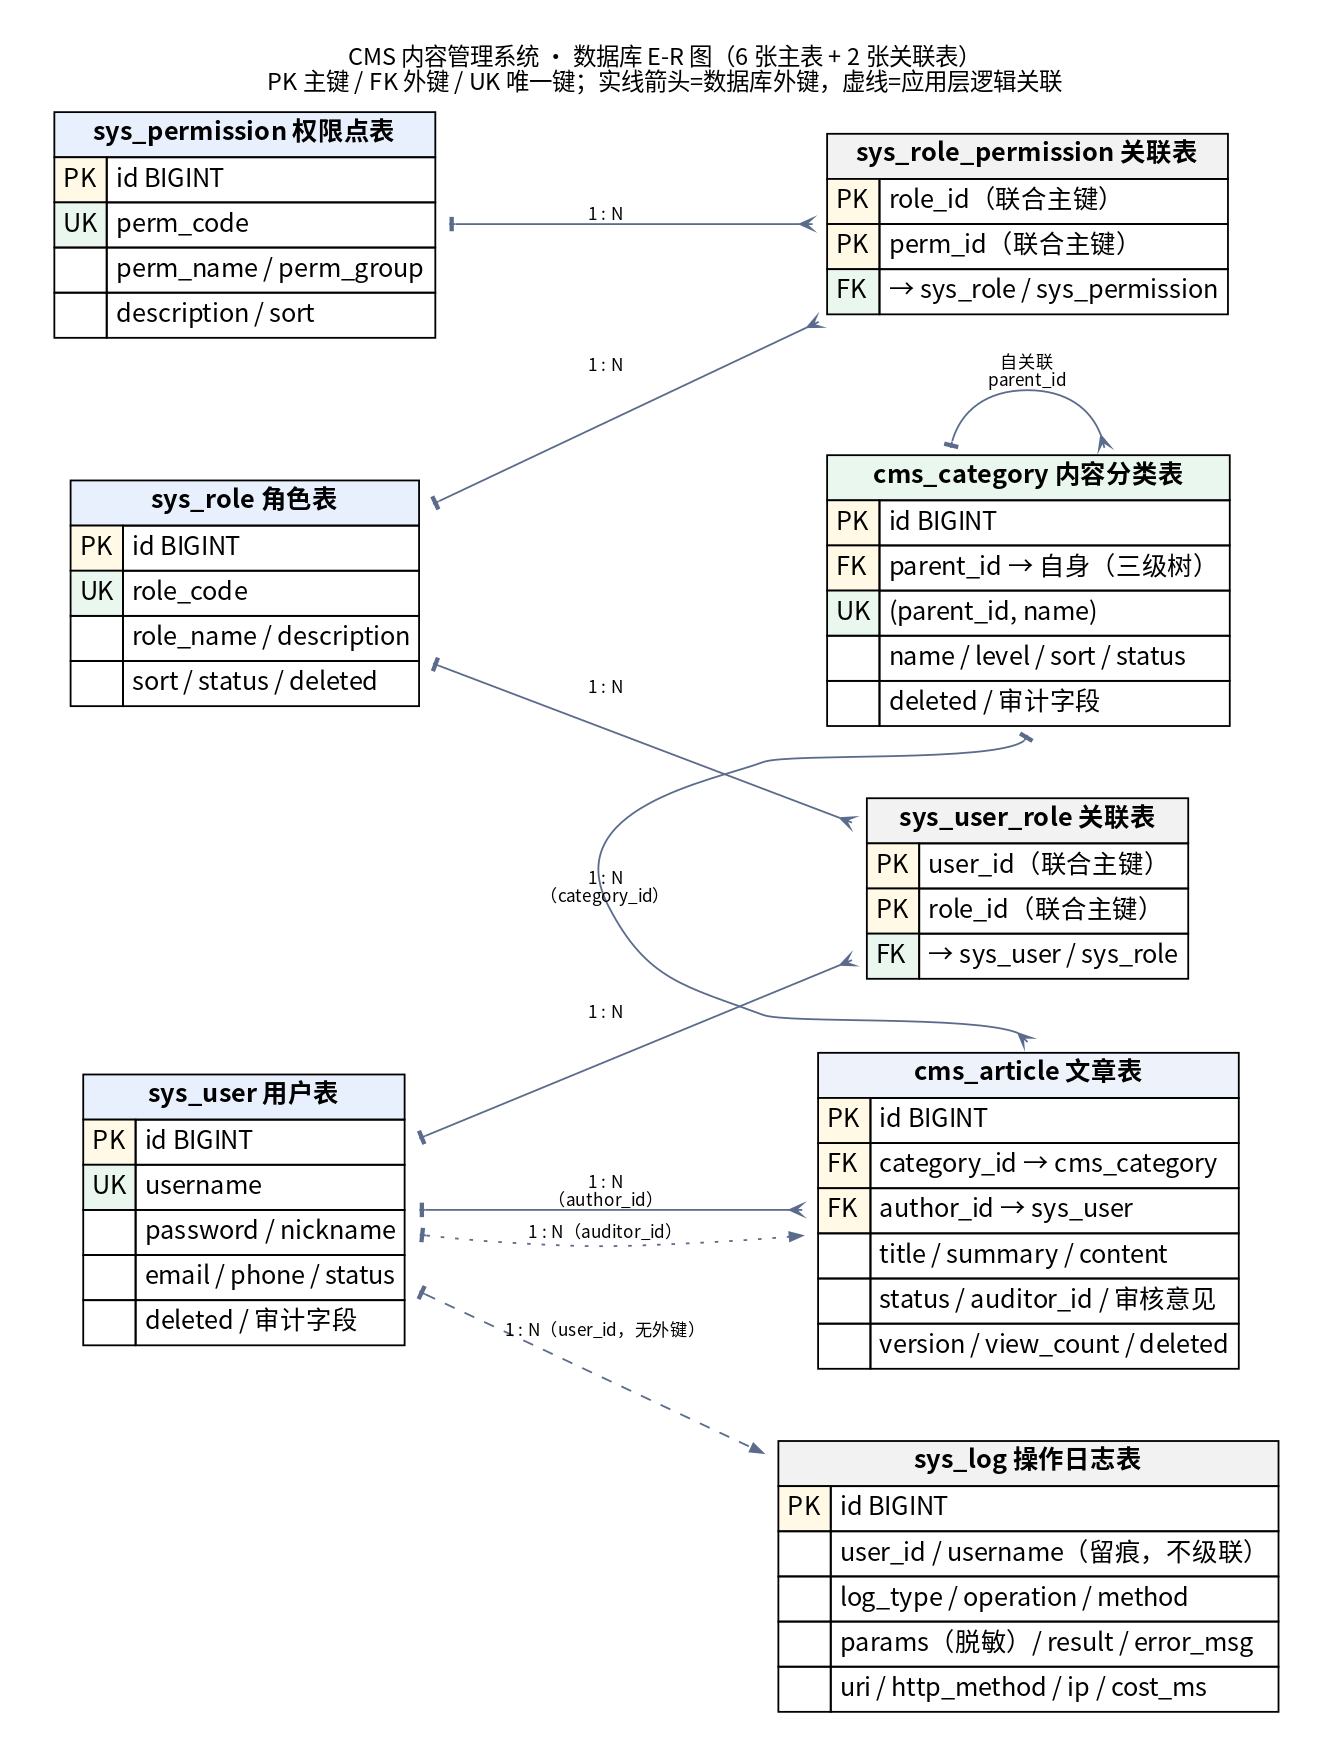
\includegraphics[width=\linewidth]{media/image1.png}

数据库 E-R 图（8 张表，标注主键 PK / 唯一键 UK / 外键 FK）

\section*{五、系统设计图}\label{ux4e94ux7cfbux7edfux8bbeux8ba1ux56fe}
\addcontentsline{toc}{section}{五、系统设计图}



\subsection*{5.1 分层架构}\label{ux5206ux5c42ux67b6ux6784}
\addcontentsline{toc}{subsection}{5.1 分层架构}

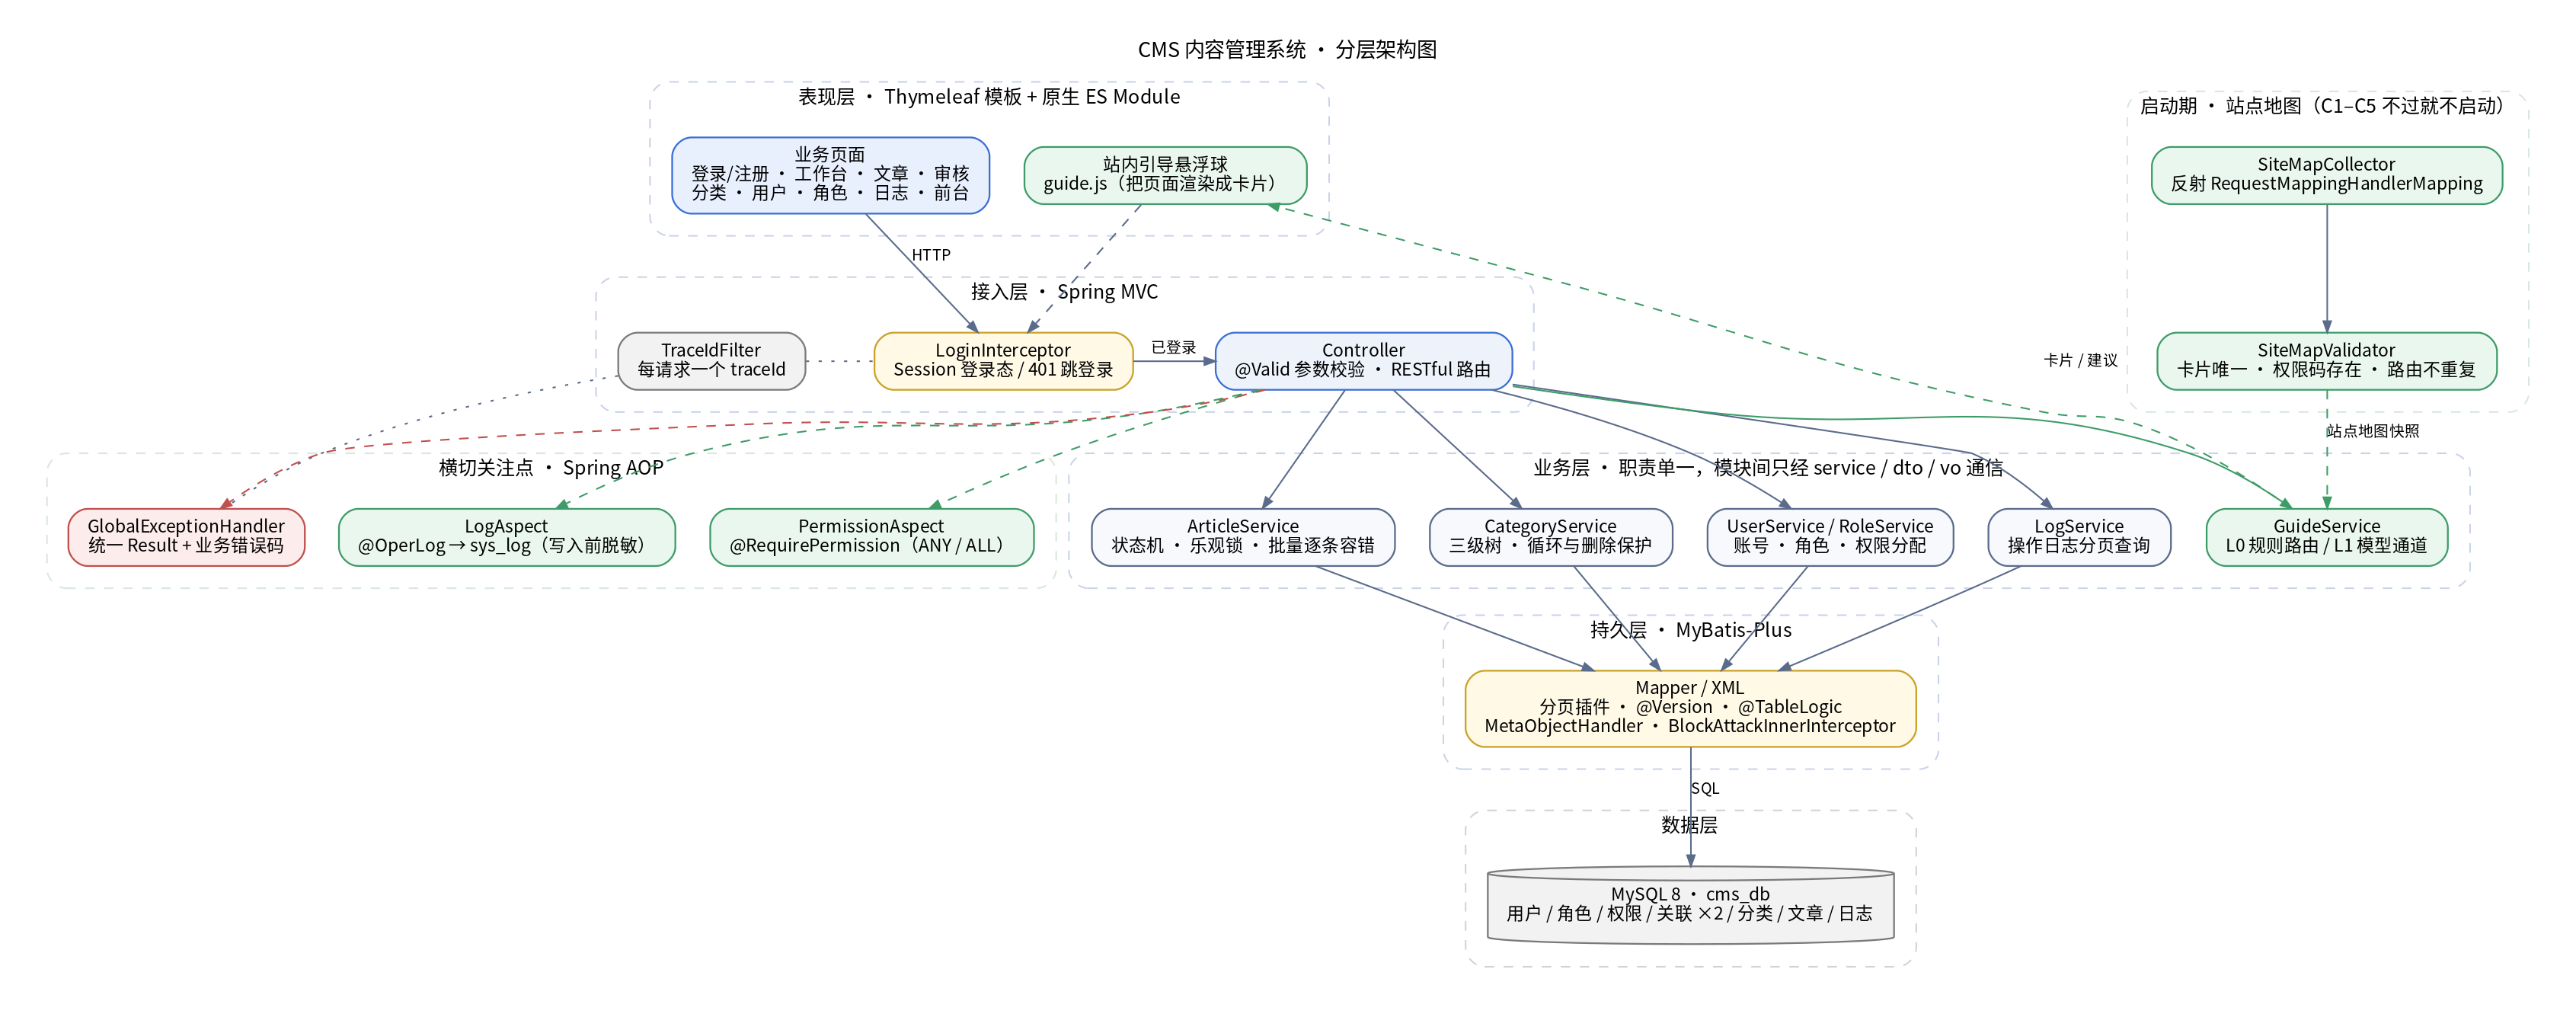
\includegraphics[width=\linewidth]{media/image2.png}

系统分层架构图

系统自上而下分为五层，依次是接入层、控制层、业务层、持久层和数据层。接入层由 Interceptor 和页面控制器构成，控制层负责参数校验与权限注解，业务层处理事务与业务规则，持久层是 Mapper 加 XML，数据层是 MySQL。横切关注点由 AOP 承担。LogAspect 在最外层，即 @Order(1)，PermissionAspect 在其内层，即 @Order(2)。因此被 403 拦下的请求仍会被日志切面看到，越权必须留痕，这个顺序本身就是一条设计决策。

\subsection*{5.2 总体业务流程}\label{ux603bux4f53ux4e1aux52a1ux6d41ux7a0b}
\addcontentsline{toc}{subsection}{5.2 总体业务流程}

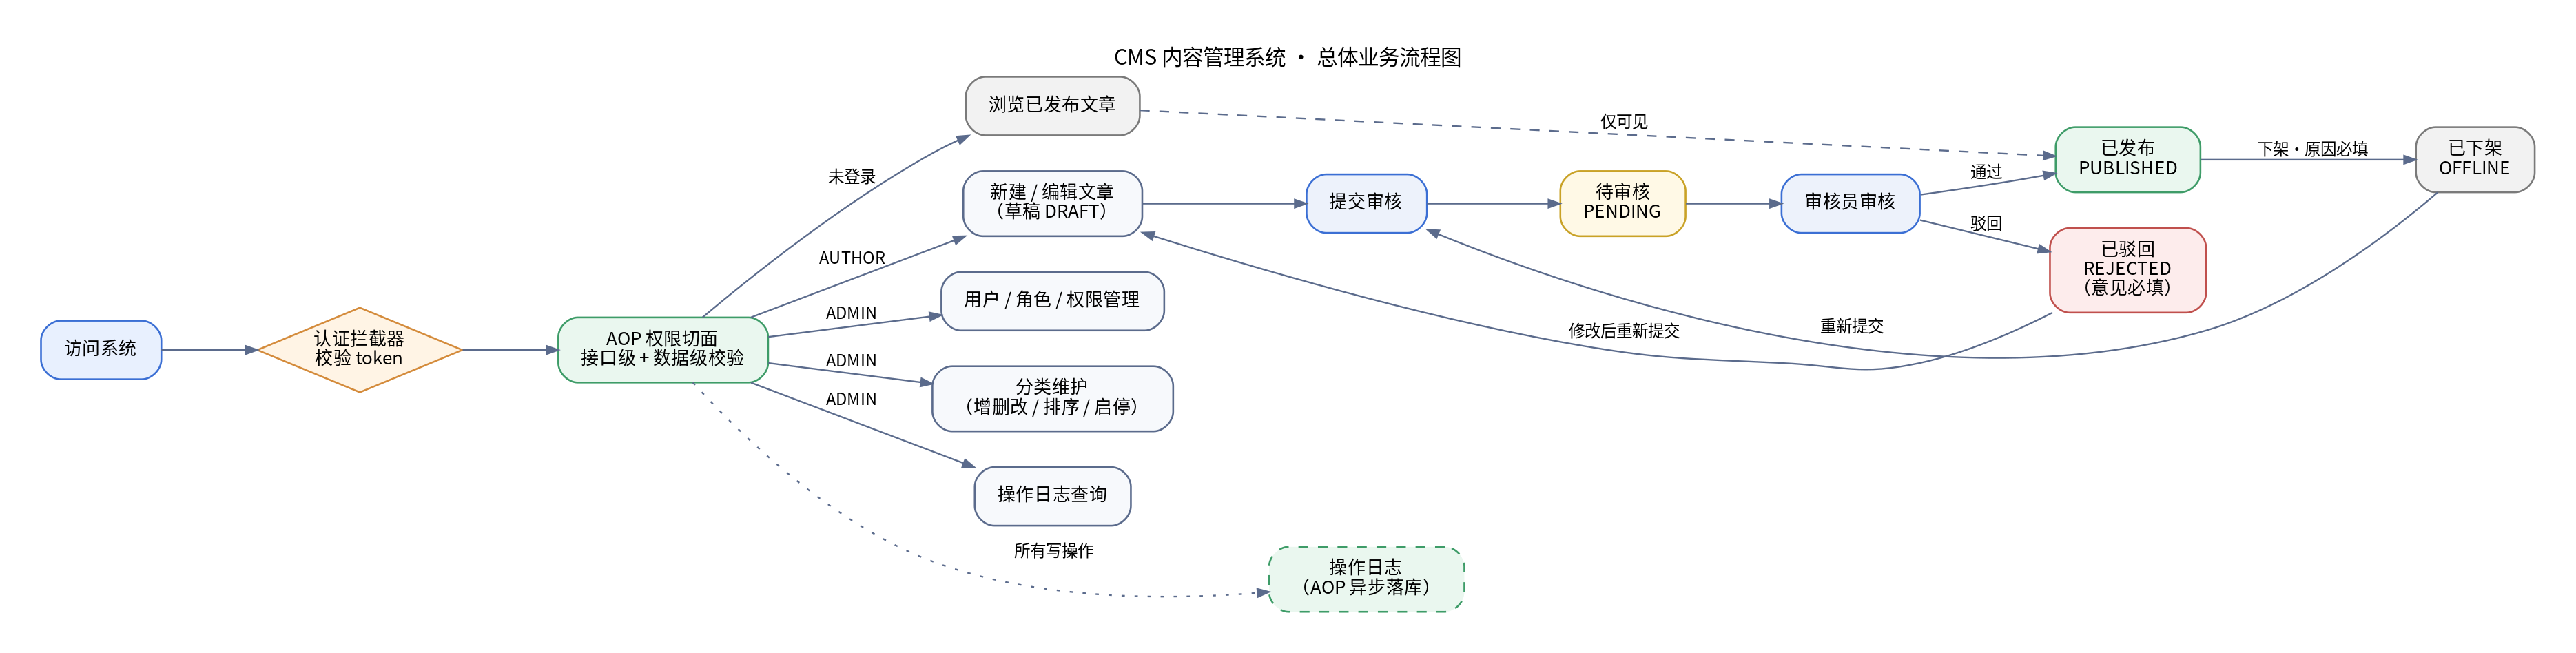
\includegraphics[width=\linewidth]{media/image3.png}

总体业务流程图

\subsection*{5.3 文章状态机}\label{ux6587ux7ae0ux72b6ux6001ux673a}
\addcontentsline{toc}{subsection}{5.3 文章状态机}

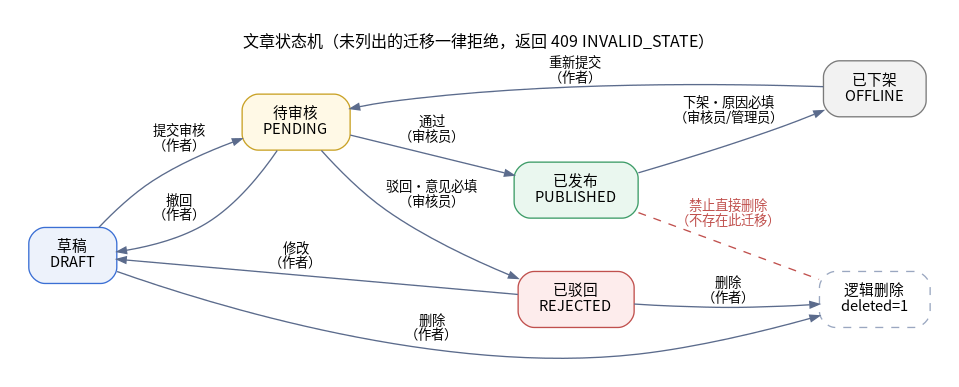
\includegraphics[width=\linewidth]{media/image4.png}

文章状态机：五态七迁

状态机是\textbf{代码里的显式表}（ArticleStateMachine），不是散落在各 Service 里的 if。next(当前状态, 动作) 查不到边就抛 BizException(INVALID\_STATE)，异常文案同时带出"当前状态"与"被拒绝的动作"。

\subsection*{5.4 站内引导时序}\label{ux7ad9ux5185ux5f15ux5bfcux65f6ux5e8f}
\addcontentsline{toc}{subsection}{5.4 站内引导时序}

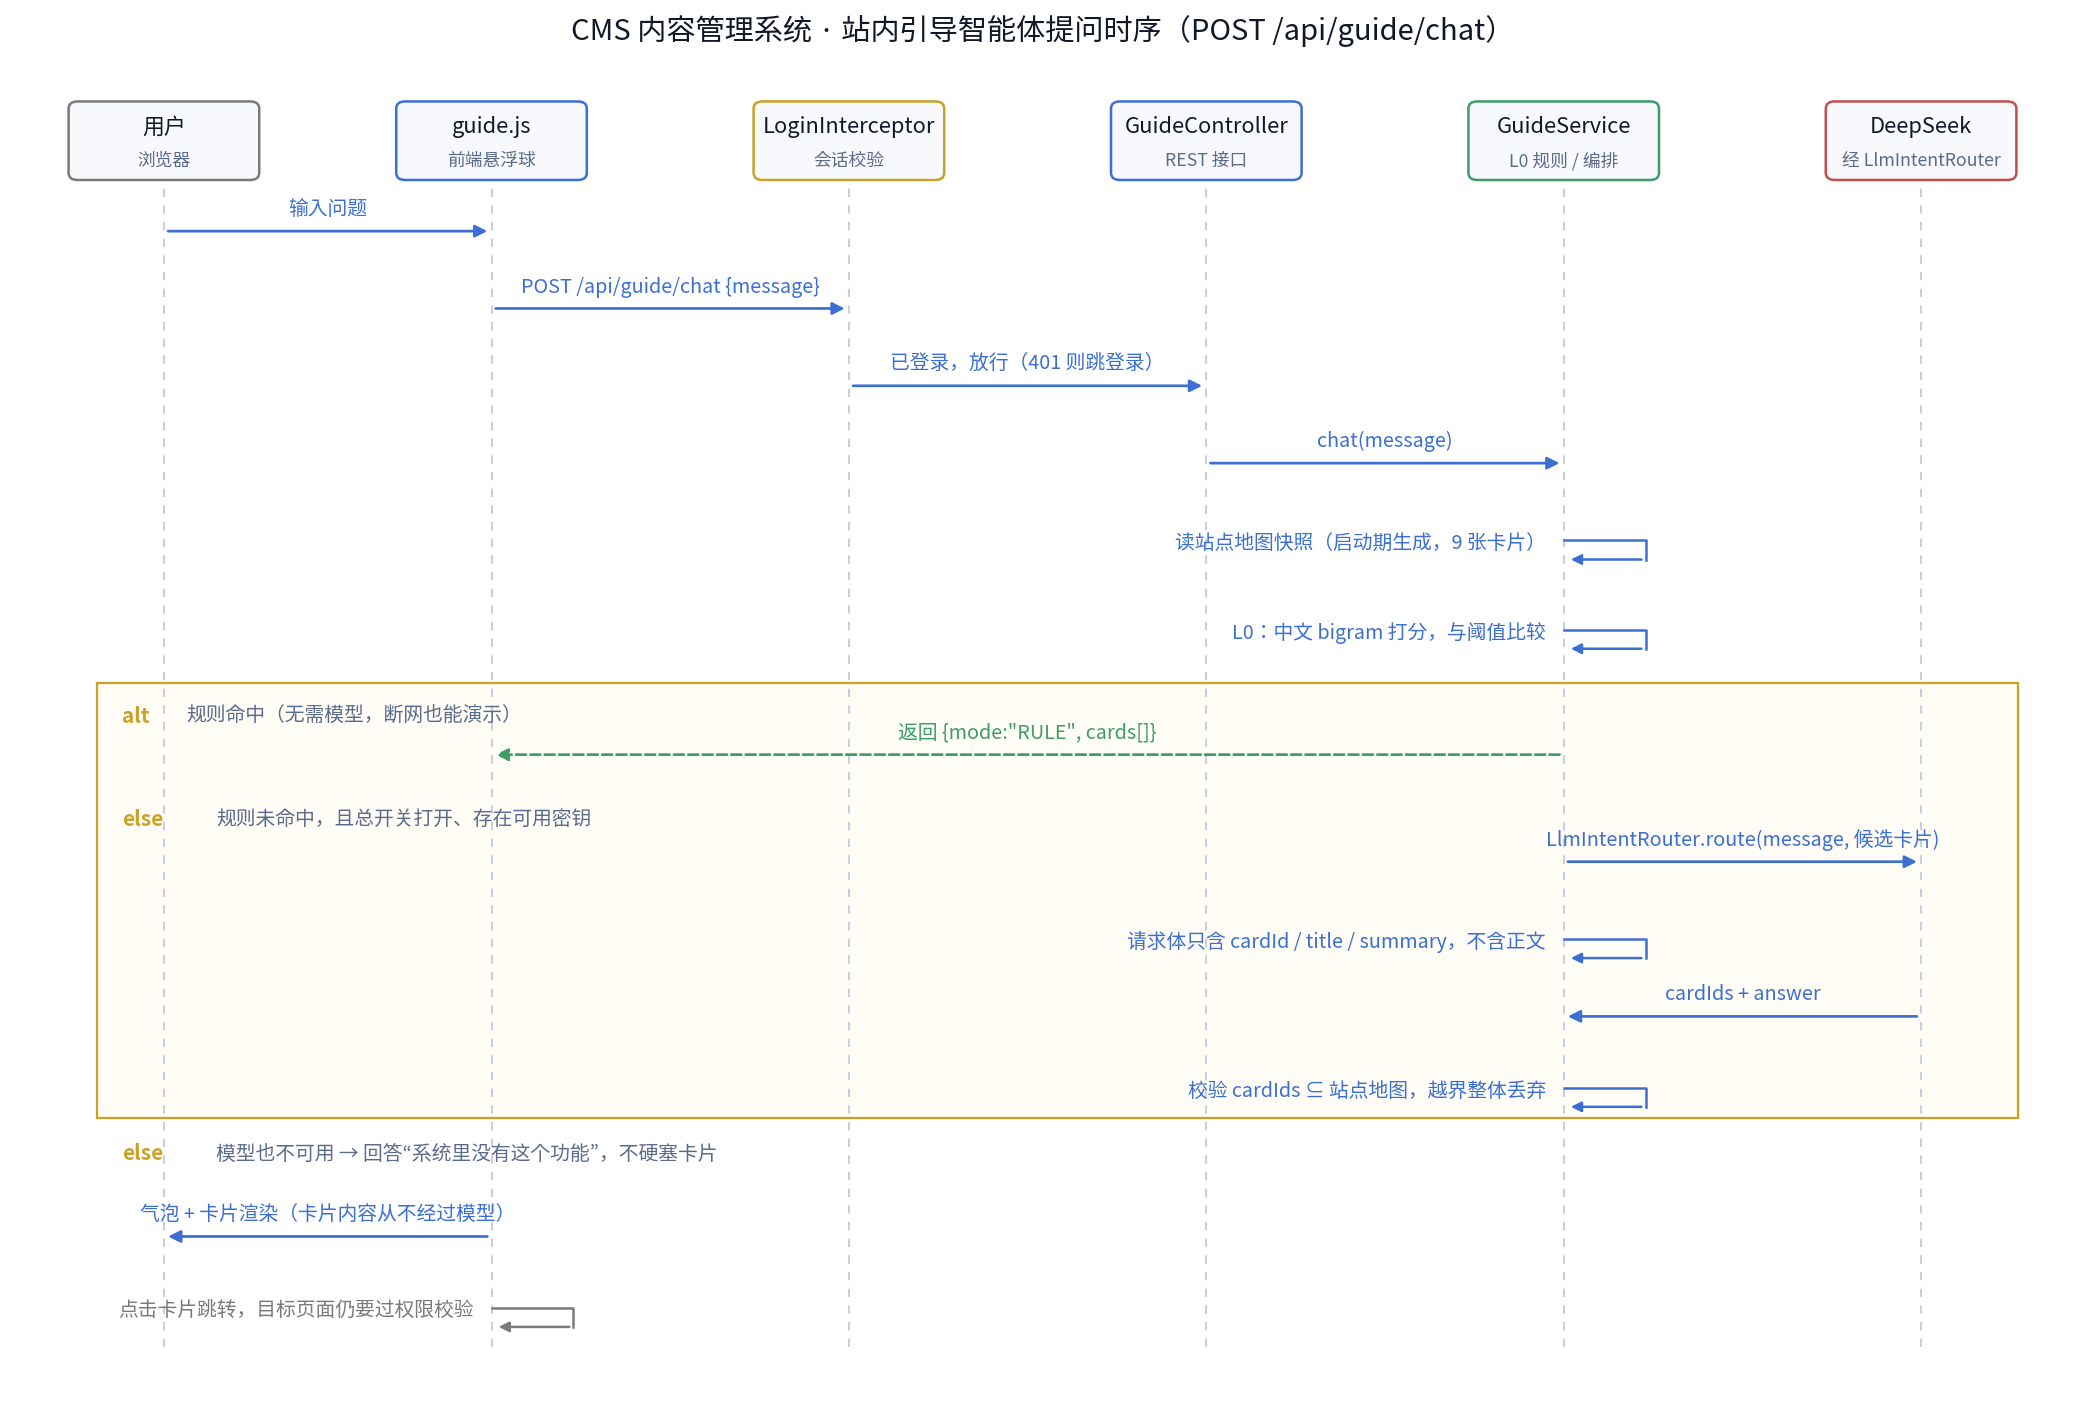
\includegraphics[width=\linewidth]{media/image5.png}

站内引导智能体时序图

一次提问的路径：前端 → GuideController.chat → IntentRouter（规则层）命中则直接返回卡片 → 未命中且模型通道开启时，把候选卡片摘要发给模型 → 模型只回卡片 id → 服务端校验 id ∈ 站点地图 → 返回渲染。

\section*{六、工程结构标准化}\label{ux516dux5de5ux7a0bux7ed3ux6784ux6807ux51c6ux5316}
\addcontentsline{toc}{section}{六、工程结构标准化}



\subsection*{6.1 目录分层}\label{ux76eeux5f55ux5206ux5c42}
\addcontentsline{toc}{subsection}{6.1 目录分层}

\begin{verbatim}
src/main/java/com/ylf/cms/
|- CmsApplication.java
|- config/ # 全局配置：MP 插件、WebMvc、自动填充
|- common/ # 无业务依赖的公共设施
| |- annotation/ # @RequirePermission、@OperLog、@GuideCard
| |- constant/ # 权限码、角色码、状态、动作枚举
| |- exception/ # BizException
| |- result/ # Result、PageResult、ResultCode
| `- util/ # SortWhitelist、MaskUtil、SensitiveInfoDetector
|- security/ # 认证与鉴权
| |- user/{controller,dto,entity,mapper,service,vo}
| |- LoginInterceptor.java
| |- PermissionAspect.java
| |- UserContext.java # ThreadLocal 当前用户
| `- LoginUser.java
|- content/ # 文章域
| `- {controller,dto,entity,mapper,service,vo}
|- catalog/ # 分类域（category）+ 前台（portal）
|- ops/ # 运维域：log（日志）+ guide（站内引导）
`- resources/
  |- mapper/ArticleMapper.xml
  |- sql/{schema.sql,data.sql}
  |- guide/site-map.yaml
  |- templates/ # 13 个 Thymeleaf 模板
  `- static/{css,js/}
\end{verbatim}

\subsection*{6.2 模块职责}\label{ux6a21ux5757ux804cux8d23}
\addcontentsline{toc}{subsection}{6.2 模块职责}

security 模块负责注册登录、会话、权限判定与越权判定，可被其他模块引用其 service、dto、vo。content 模块负责文章生命周期、检索、批量与敏感信息，依赖 security 的 LoginUser。catalog 模块负责分类树与前台阅读站，依赖 content 展示文章。ops 模块负责操作日志与站内引导，读其他模块的 service，不读其 mapper。

\subsection*{6.3 模块边界检查}\label{ux8fb9ux754cux5224ux636e}
\addcontentsline{toc}{subsection}{6.3 模块边界检查}

项目通过 ModuleBoundaryTest 扫描源码中的 import，检查业务模块是否跨层引用其他模块的 Mapper、实体、控制器或配置类，公共交互按约定经过 service、dto 和 vo。

原测试曾因包路径层级判断错误，未识别 security.user.mapper 中的越界引用。定位问题后调整了路径解析，并加入违规引用验证检测是否生效。边界测试本身也需要反例，测试通过只能说明已覆盖的检查项满足要求。

\section*{七、基础核心功能}\label{ux4e03ux529fux80fdux5b9eux73b0ux8be6ux89e3}
\addcontentsline{toc}{section}{七、基础核心功能}



\subsection*{7.1 用户权限管理}\label{ux7528ux6237ux6743ux9650ux7ba1ux7406}
\addcontentsline{toc}{subsection}{7.1 用户权限管理}

账号全生命周期与权限控制分注册、登录、退出、角色分配、AOP 权限校验五部分，各部分功能截屏如下。

本模块涉及认证、用户、角色三组接口，接口名称与功能说明如下表。

\begin{longtable}{@{}>{\raggedright\arraybackslash}p{8.4cm}>{\raggedright\arraybackslash}p{4.4cm}@{}}
\toprule
\textbf{接口名称} & \textbf{功能说明} \\
\midrule
\endfirsthead
\multicolumn{2}{@{}l}{\small（续表）}\\
\toprule
\textbf{接口名称} & \textbf{功能说明} \\
\midrule
\endhead
\multicolumn{2}{@{}l}{\textbf{认证} \quad /api/auth} \\
\midrule
POST /api/auth/register & 注册账号，默认挂 AUTHOR 角色 \\
POST /api/auth/login & 登录系统，返回角色与权限 \\
POST /api/auth/logout & 退出登录，销毁 Session \\
GET /api/auth/me & 查询当前用户及权限 \\
\multicolumn{2}{@{}l}{\textbf{用户} \quad /api/users} \\
\midrule
GET /api/users & 分页查询用户 \\
GET /api/users/\{id\} & 查询用户详情 \\
POST /api/users & 新增用户 \\
PUT /api/users/\{id\} & 修改用户资料 \\
PUT /api/users/\{id\}/status & 启用或停用用户 \\
PUT /api/users/\{id\}/roles & 分配用户角色 \\
DELETE /api/users/\{id\} & 删除用户 \\
\multicolumn{2}{@{}l}{\textbf{角色} \quad /api/roles} \\
\midrule
GET /api/roles & 查询角色列表 \\
GET /api/roles/permissions & 查询全部权限点 \\
POST /api/roles & 新增角色 \\
PUT /api/roles/\{id\} & 修改角色 \\
PUT /api/roles/\{id\}/permissions & 分配角色权限 \\
DELETE /api/roles/\{id\} & 删除角色 \\
\bottomrule
\end{longtable}

请求数据结构（DTO）直接取自代码：注册用 RegisterRequest，用户管理用 UserSaveRequest。

\begin{verbatim}
public class RegisterRequest {
    @NotBlank(message = "用户名不能为空")
    @Pattern(regexp = "^[a-zA-Z0-9_]{4,20}$", message = "用户名为 4-20 位字母、数字或下划线")
    private String username;

    @NotBlank(message = "密码不能为空")
    @Size(min = 6, max = 32, message = "密码长度 6-32 位")
    private String password;

    @NotBlank(message = "昵称不能为空")
    @Size(max = 50, message = "昵称最长 50 字")
    private String nickname;

    @Email(message = "邮箱格式不正确")
    private String email;
}
\end{verbatim}

\begin{verbatim}
public class UserSaveRequest {
    @Pattern(regexp = "^[a-zA-Z0-9_]{4,20}$", message = "用户名为 4-20 位字母、数字或下划线")
    private String username;   // 新增必填，修改时忽略

    @Size(min = 6, max = 32, message = "密码长度 6-32 位")
    private String password;   // 修改时留空表示不改密码

    @NotBlank(message = "昵称不能为空")
    private String nickname;

    @Email(message = "邮箱格式不正确")
    private String email;

    private List<Long> roleIds;
}
\end{verbatim}

登录处理流程如下。

\begin{center}
\begin{tikzpicture}[
  node distance=5mm,
  box/.style={rectangle, draw, rounded corners=1pt, align=center, minimum width=5.4cm, minimum height=0.72cm, font=\small},
  arr/.style={-{Stealth}}
]
\node[box] (a) {POST /api/auth/login 收到登录请求};
\node[box, below=of a] (b) {查用户、比对 BCrypt 密码、校验 status=1};
\node[box, below=of b] (c) {装配角色集合与权限集合到 LoginUser};
\node[box, below=of c] (d) {写入 Session，返回当前用户};
\draw[arr] (a) -- (b);
\draw[arr] (b) -- (c);
\draw[arr] (c) -- (d);
\end{tikzpicture}
\end{center}

\subsubsection*{7.1.1 注册}\label{sec:reg}
\addcontentsline{toc}{subsubsection}{7.1.1 注册}

注册时，RegisterRequest 用 @Valid 校验用户名格式、密码长度和邮箱格式。用户名重复先查一次，并发下由唯一索引兜底。密码用 BCryptPasswordEncoder 加密。插入后自动挂上 RoleCode.DEFAULT，即 AUTHOR 角色。

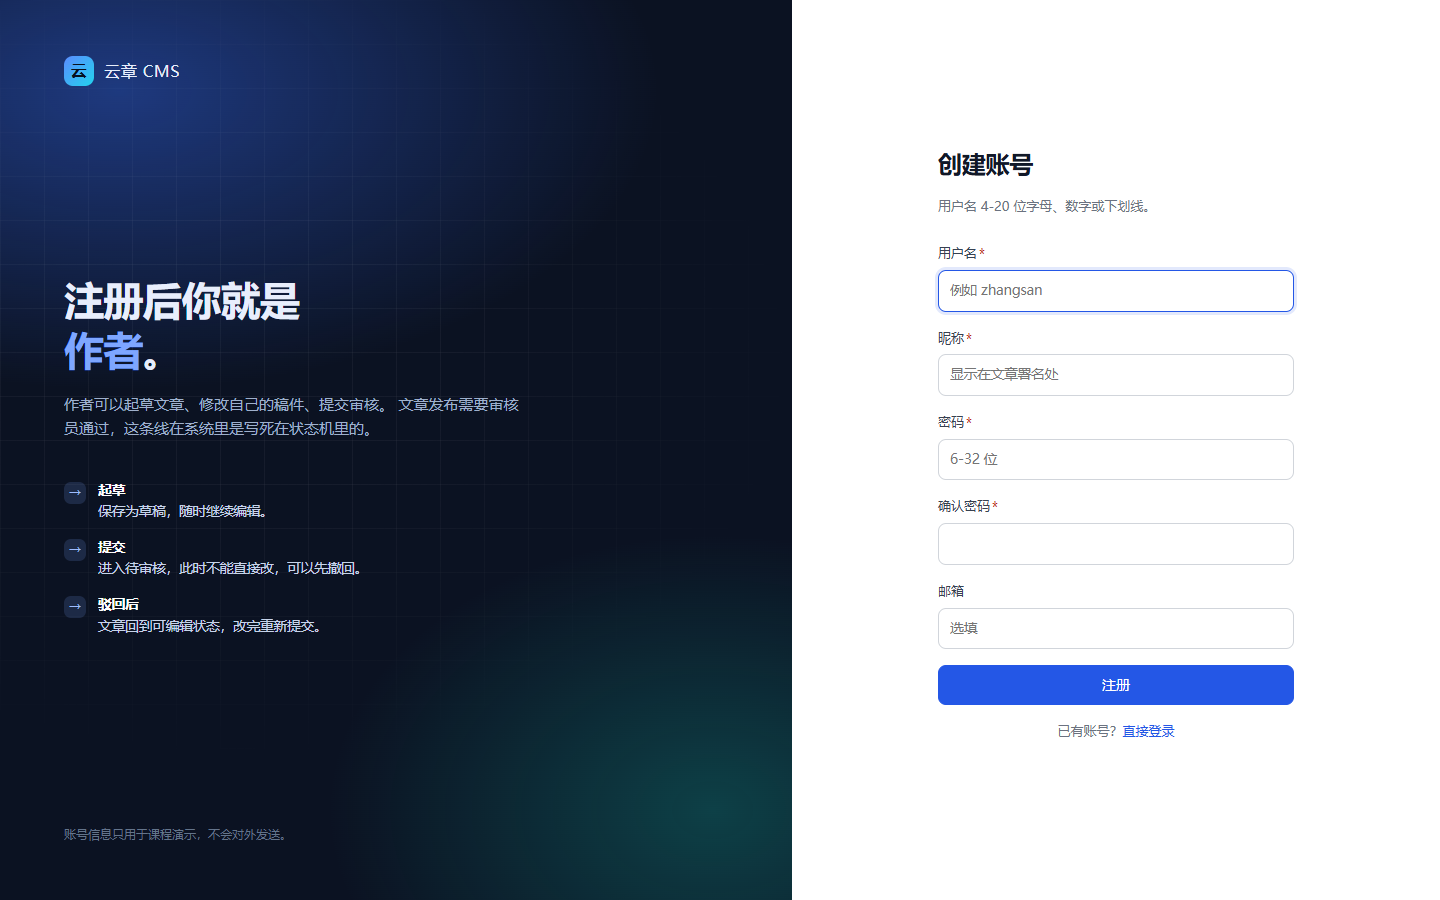
\includegraphics[width=\linewidth]{media/image16.png}

\subsubsection*{7.1.2 登录}\label{sec:login}
\addcontentsline{toc}{subsubsection}{7.1.2 登录}

登录时校验用户存在、密码匹配、status 为 1，然后把角色集合与权限集合装配进 LoginUser 存入 Session。权限在登录时一次性算好，请求期间不再查库。密码错误与用户不存在返回同一错误码 40101，避免账号枚举。

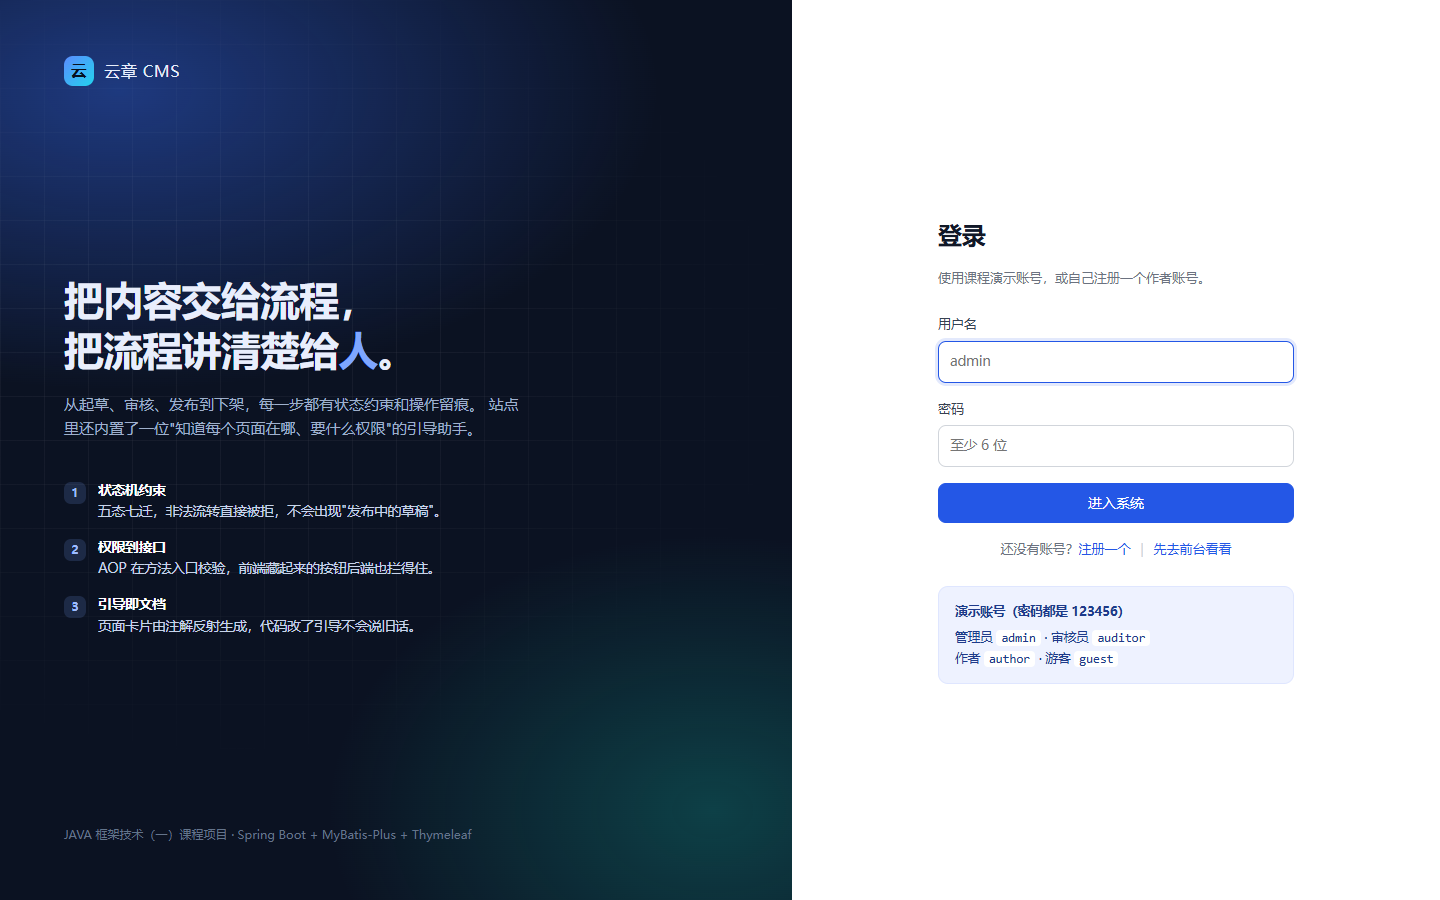
\includegraphics[width=\linewidth]{media/image17.png}

\subsubsection*{7.1.3 退出}\label{sec:logout}
\addcontentsline{toc}{subsubsection}{7.1.3 退出}

退出时调用 session.invalidate()，返回统一的 Result 结果。

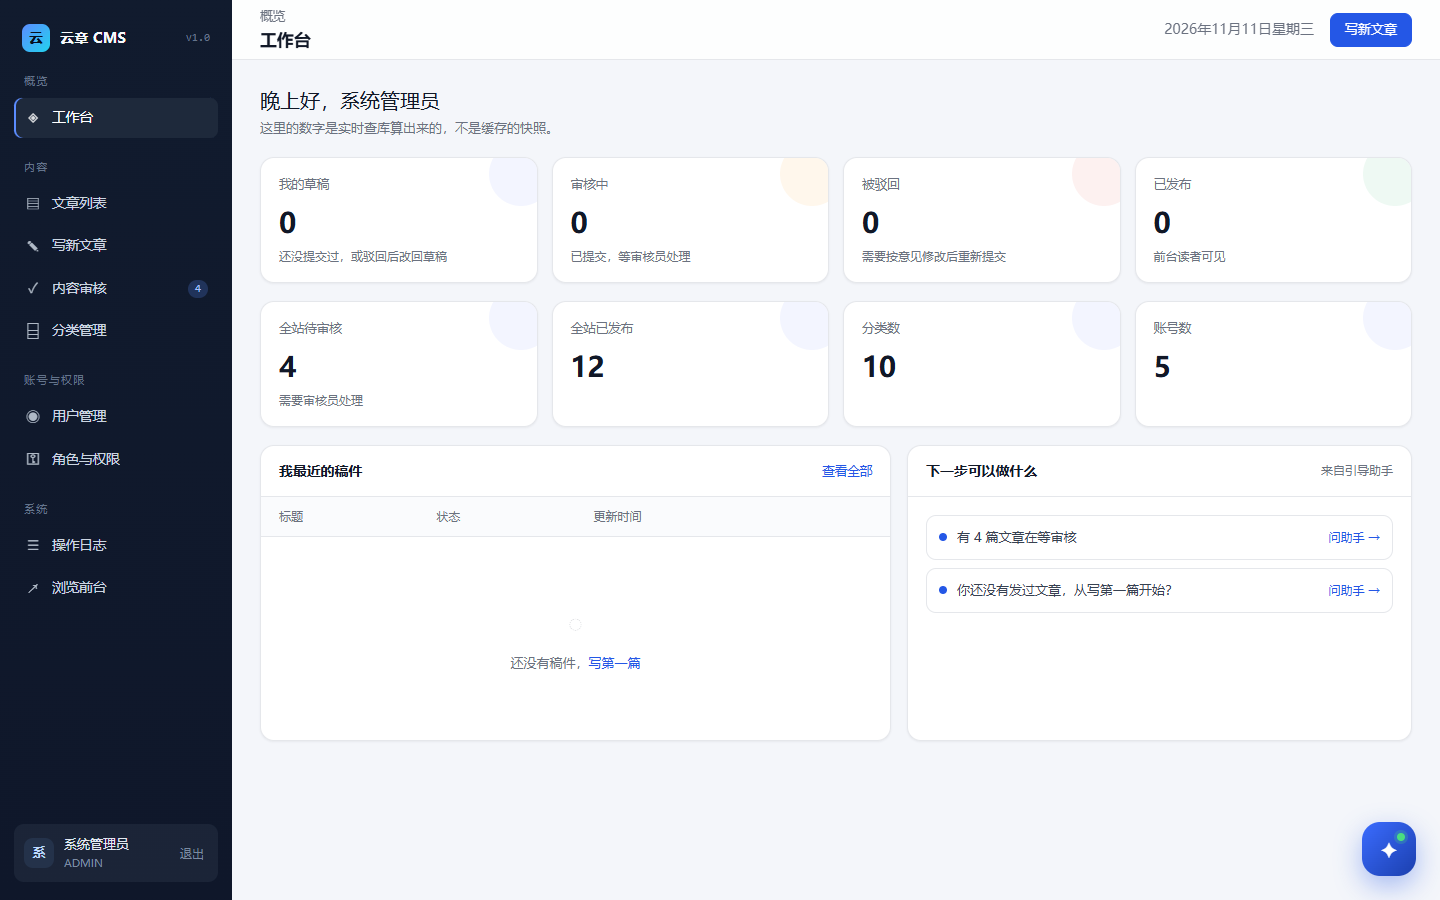
\includegraphics[width=\linewidth]{media/image18.png}

\subsubsection*{7.1.4 角色分配}\label{sec:role}
\addcontentsline{toc}{subsubsection}{7.1.4 角色分配}

角色分配由 PUT /api/users/\{id\}/roles 完成，全量覆盖用户的角色列表，管理员可随时调整。角色的权限点由 PUT /api/roles/\{id\}/permissions 全量覆盖式保存。

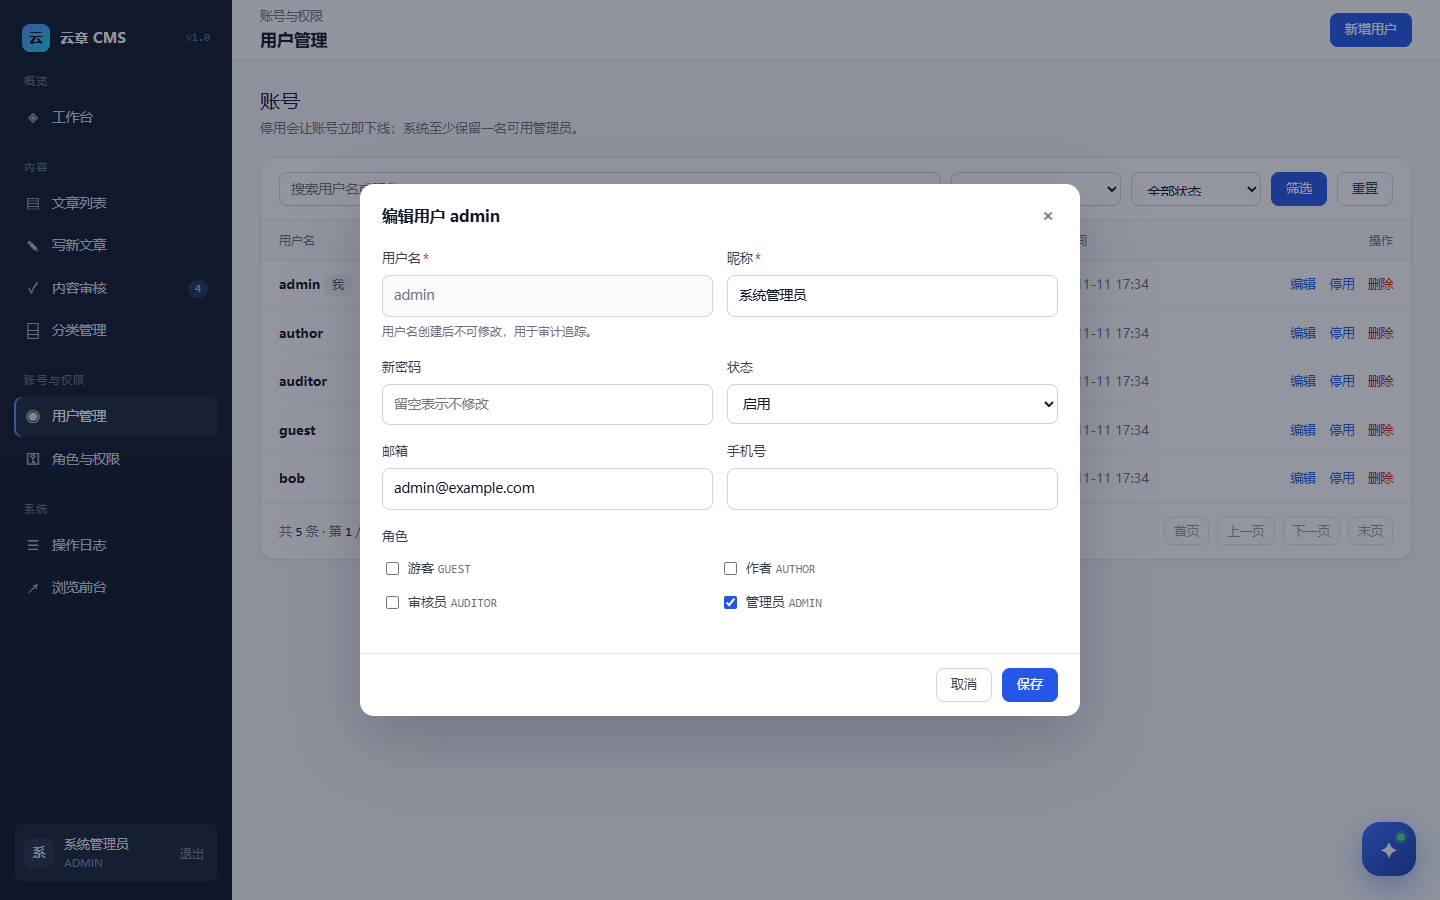
\includegraphics[width=\linewidth]{media/image19.png}

\subsubsection*{7.1.5 AOP 权限校验}\label{sec:aop}
\addcontentsline{toc}{subsubsection}{7.1.5 AOP 权限校验}

接口级权限由控制器方法标注 @RequirePermission(Perm.ARTICLE\_AUDIT) 实现。切面读取注解并与权限集合比对，支持 ANY 和 ALL 两种逻辑，ANY 是默认值，任一命中即通过，ALL 要求全部命中。判断逻辑如下：

boolean allowed = requirePermission.logic() == RequirePermission.Logic.ALL\\
? Arrays.stream(codes).allMatch(user::hasPermission)\\
: user.hasAnyPermission(codes);\\
if (!allowed) \{\\
throw new BizException(ResultCode.FORBIDDEN, "缺少权限：" + String.join(" 或 ", codes));\\
\}

数据级权限解决接口级权限回答不了的问题。接口级只能回答这个角色能不能调这个接口，而作者 A 能不能改作者 B 的稿是数据级问题。数据级判断在 Service 里用 checkOwner 完成，有 :any 权限直接放行，否则必须满足 article.authorId 等于当前用户 id，不满足返回 403 和 40301。两层分工是刻意的。只用 AOP 拿不到数据行，只在 Service 判断则每个接口都要重复写。

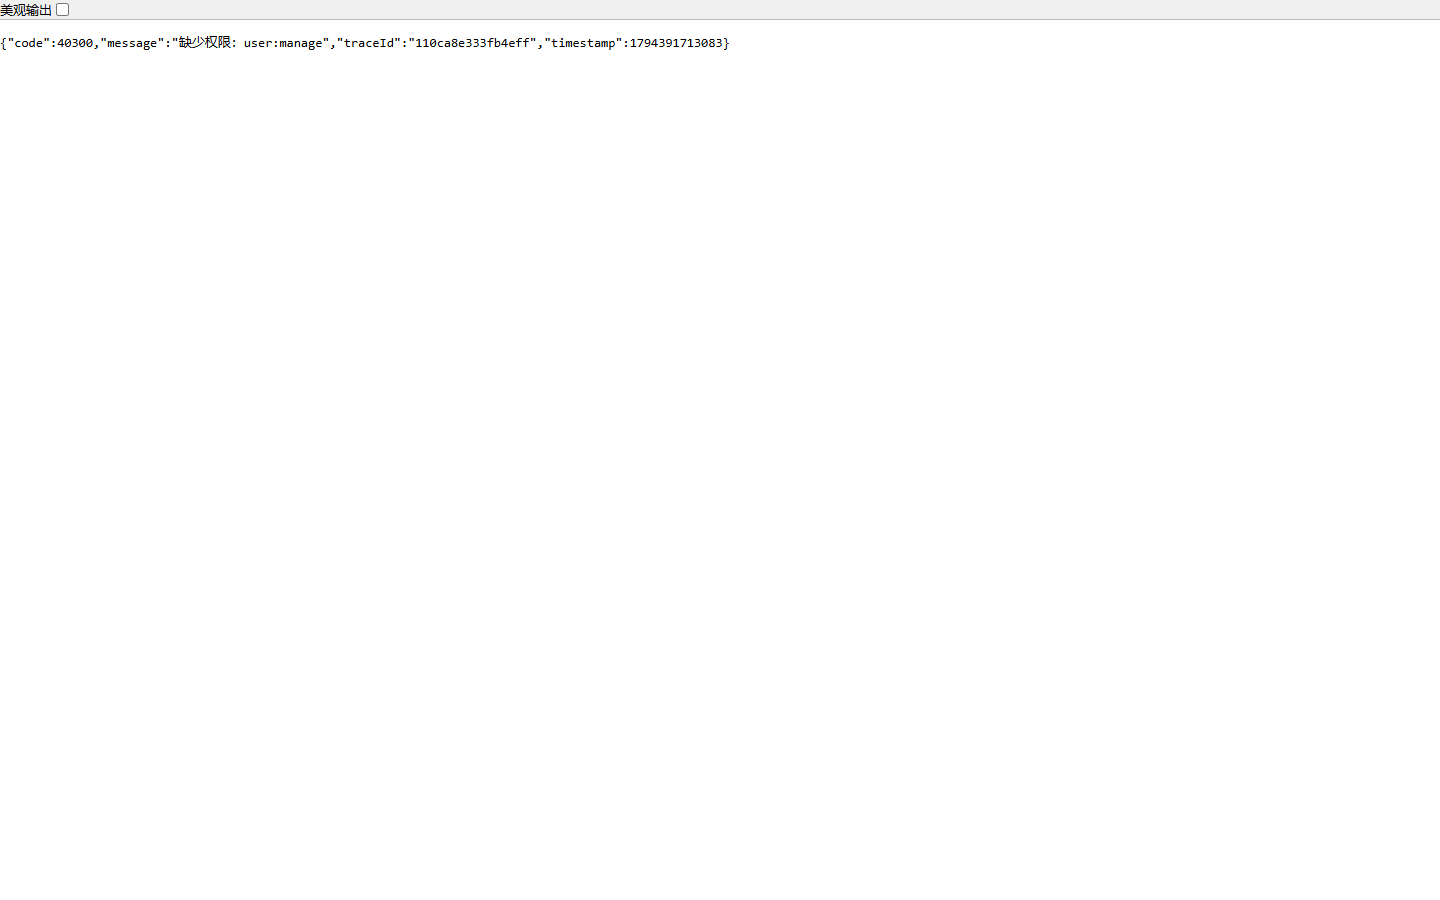
\includegraphics[width=\linewidth]{media/image20.png}

\subsection*{7.2 内容分类管理}\label{ux5185ux5bb9ux5206ux7c7bux7ba1ux7406}
\addcontentsline{toc}{subsection}{7.2 内容分类管理}

分类层级用 level 字段显式存储，查树按 parent\_id 逐层展开，不做递归查库。level 由服务端根据父节点推导，不信任客户端传入。以下按新增、编辑、排序、删除、状态启停、分类与内容关联绑定分述。

本模块涉及分类与前台两组接口，接口名称与功能说明如下表。

\begin{longtable}{@{}>{\raggedright\arraybackslash}p{8.4cm}>{\raggedright\arraybackslash}p{4.4cm}@{}}
\toprule
\textbf{接口名称} & \textbf{功能说明} \\
\midrule
\endfirsthead
\multicolumn{2}{@{}l}{\small（续表）}\\
\toprule
\textbf{接口名称} & \textbf{功能说明} \\
\midrule
\endhead
\multicolumn{2}{@{}l}{\textbf{分类} \quad /api/categories} \\
\midrule
GET /api/categories/tree & 查询分类树 \\
GET /api/categories & 查询分类列表 \\
POST /api/categories & 新增分类 \\
PUT /api/categories/\{id\} & 修改分类 \\
PUT /api/categories/\{id\}/status & 启用或停用分类 \\
DELETE /api/categories/\{id\} & 删除分类 \\
\multicolumn{2}{@{}l}{\textbf{前台（免登录）} \quad /api/portal} \\
\midrule
GET /api/portal/articles & 查询前台已发布文章 \\
GET /api/portal/articles/\{id\} & 查询前台文章正文 \\
GET /api/portal/categories & 查询前台启用分类树 \\
\bottomrule
\end{longtable}

请求数据结构（DTO）直接取自代码。

\begin{verbatim}
public class CategorySaveRequest {
    private Long parentId;     // 0 表示根节点

    @NotBlank(message = "分类名称不能为空")
    @Size(max = 50, message = "分类名称最长 50 字")
    private String name;

    private Integer sort;

    @NotNull(message = "状态不能为空")
    private Integer status;
}
\end{verbatim}

分类新增处理流程如下。

\begin{center}
\begin{tikzpicture}[
  node distance=5mm,
  box/.style={rectangle, draw, rounded corners=1pt, align=center, minimum width=5.6cm, minimum height=0.72cm, font=\small},
  arr/.style={-{Stealth}}
]
\node[box] (a) {POST /api/categories 收到新增请求};
\node[box, below=of a] (b) {@Valid 校验名称与状态};
\node[box, below=of b] (c) {按父节点推导 level，检查层级上限};
\node[box, below=of c] (d) {唯一索引 uk\_category\_parent\_name 兜底重名};
\node[box, below=of d] (e) {入库并返回分类 id};
\draw[arr] (a) -- (b);
\draw[arr] (b) -- (c);
\draw[arr] (c) -- (d);
\draw[arr] (d) -- (e);
\end{tikzpicture}
\end{center}

\subsubsection*{7.2.1 分类新增}\label{sec:cate-add}
\addcontentsline{toc}{subsubsection}{7.2.1 分类新增}

新增分类时，同级重名由 uk\_category\_parent\_name 兜底，服务层把唯一键冲突翻译成 40902。

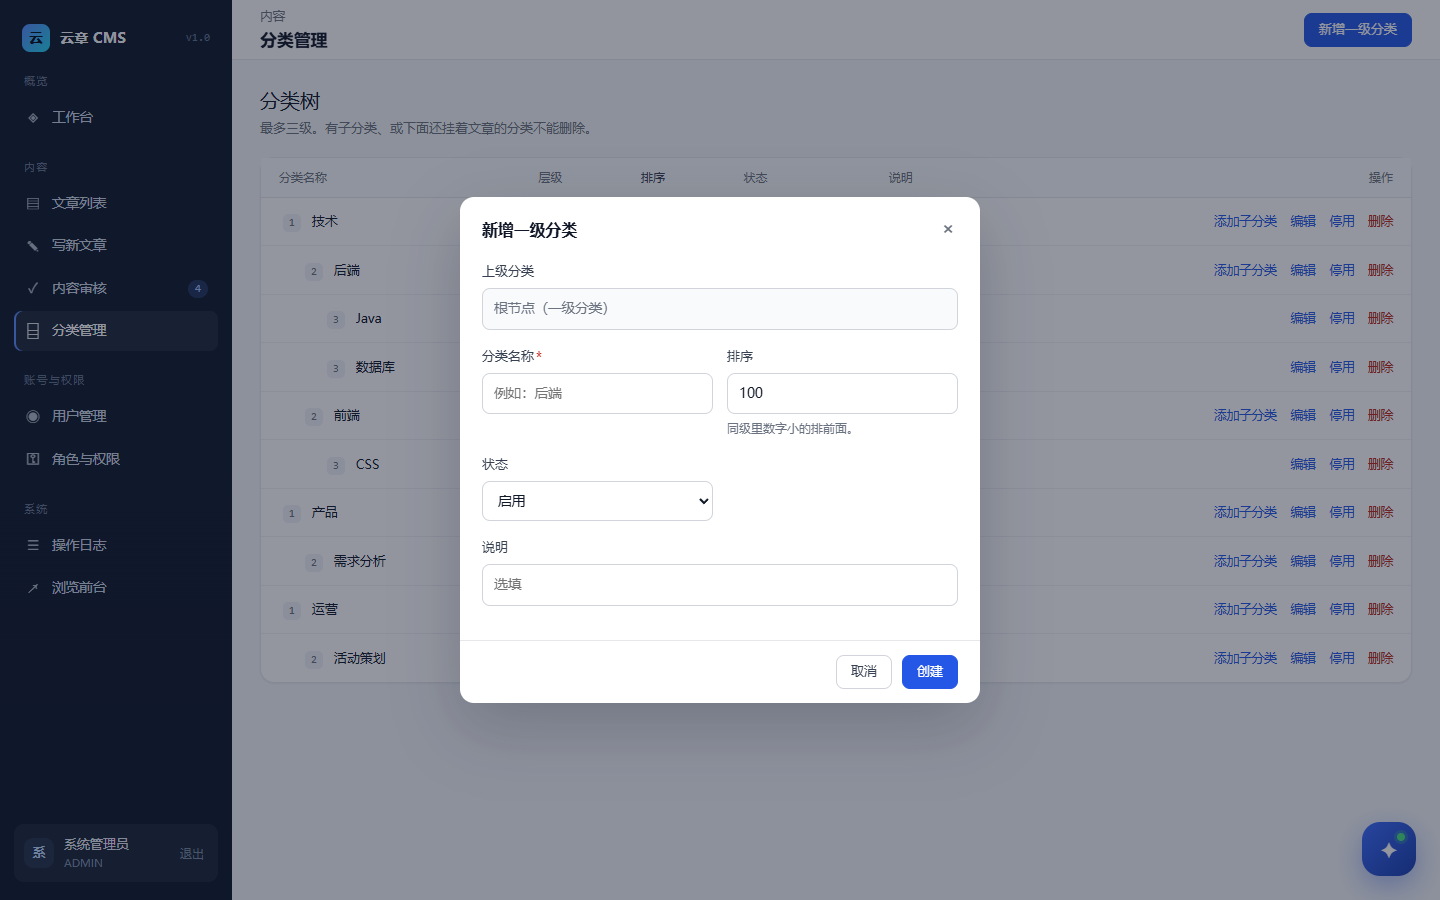
\includegraphics[width=\linewidth]{media/image21.png}

\subsubsection*{7.2.2 分类编辑}\label{sec:cate-edit}
\addcontentsline{toc}{subsubsection}{7.2.2 分类编辑}

编辑时接口忽略 parentId，不支持更换上级，避免 level 冗余字段的级联更新。

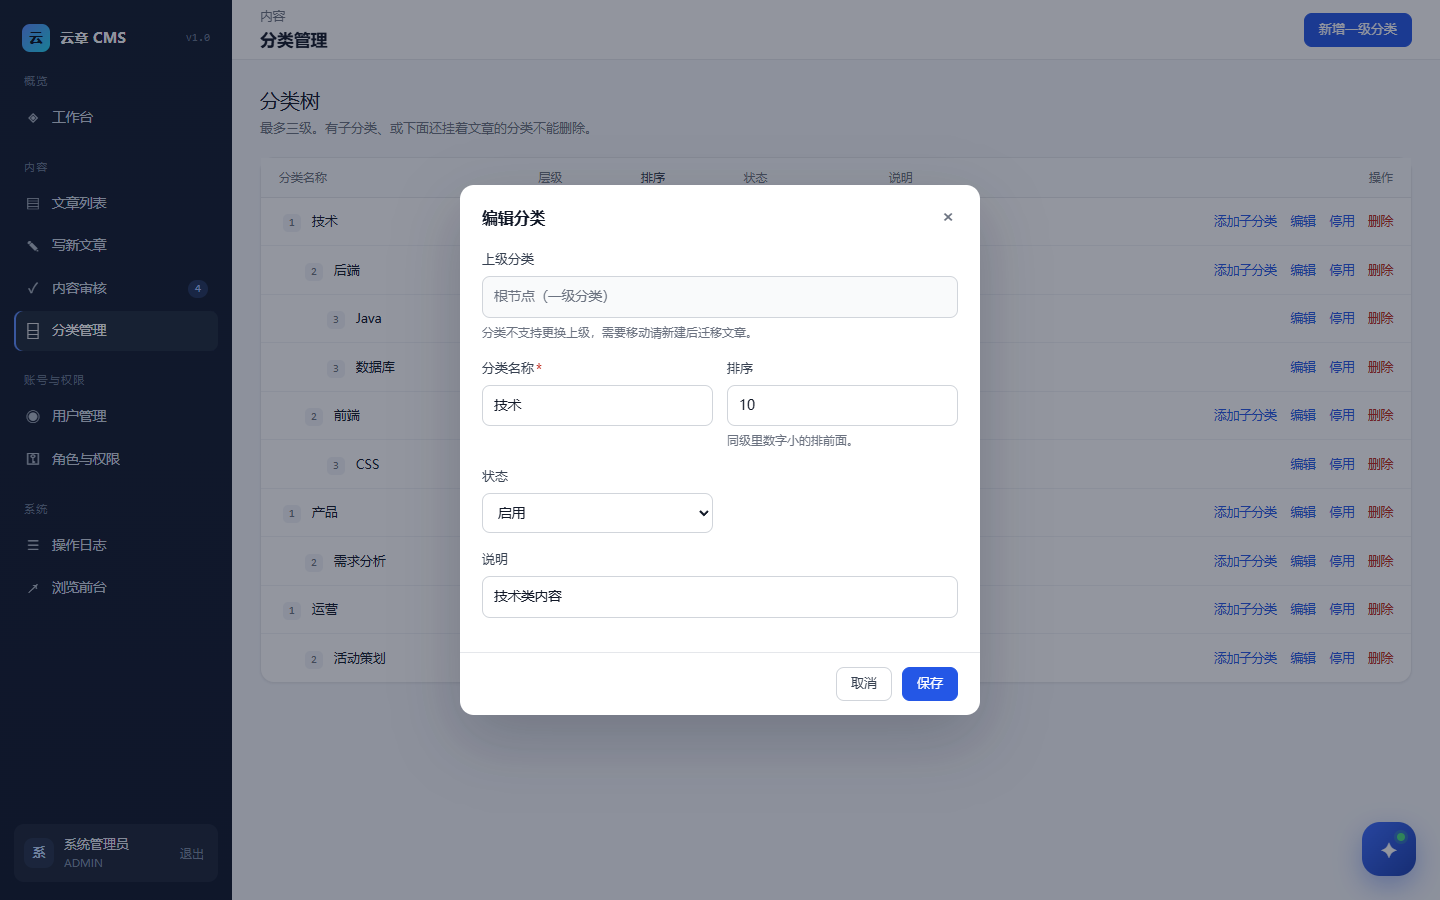
\includegraphics[width=\linewidth]{media/image22.png}

\subsubsection*{7.2.3 分类排序}\label{sec:cate-sort}
\addcontentsline{toc}{subsubsection}{7.2.3 分类排序}

排序使用 sort 字段在同级内排序，列表按 sort ASC 加 id ASC 保证稳定。

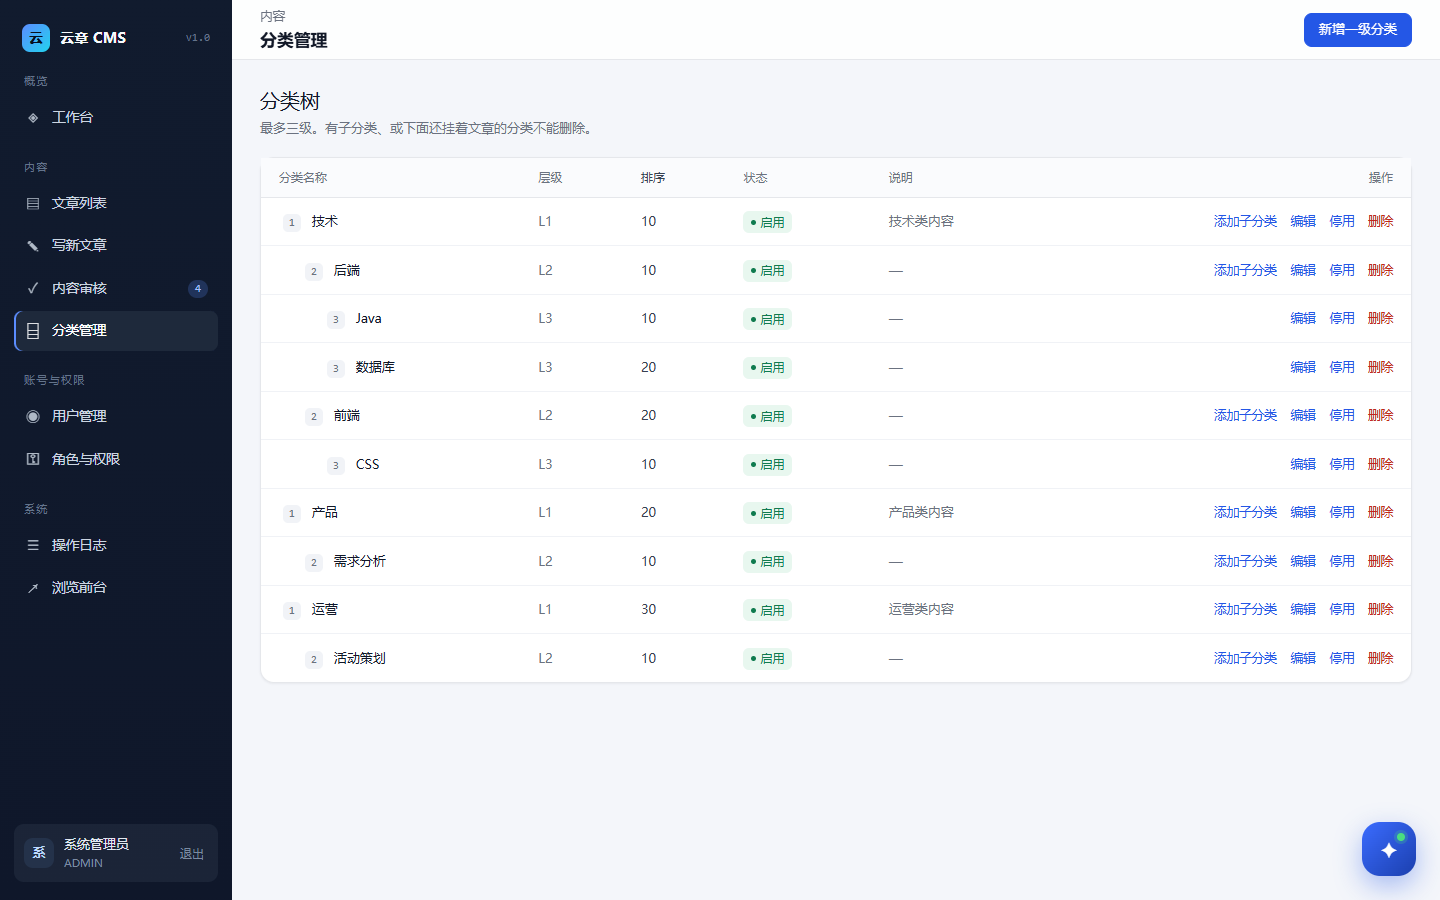
\includegraphics[width=\linewidth]{media/image23.png}

\subsubsection*{7.2.4 分类删除}\label{sec:cate-del}
\addcontentsline{toc}{subsubsection}{7.2.4 分类删除}

删除前检查子分类与引用文章，任何一个存在就返回 40903，不做级联删除。

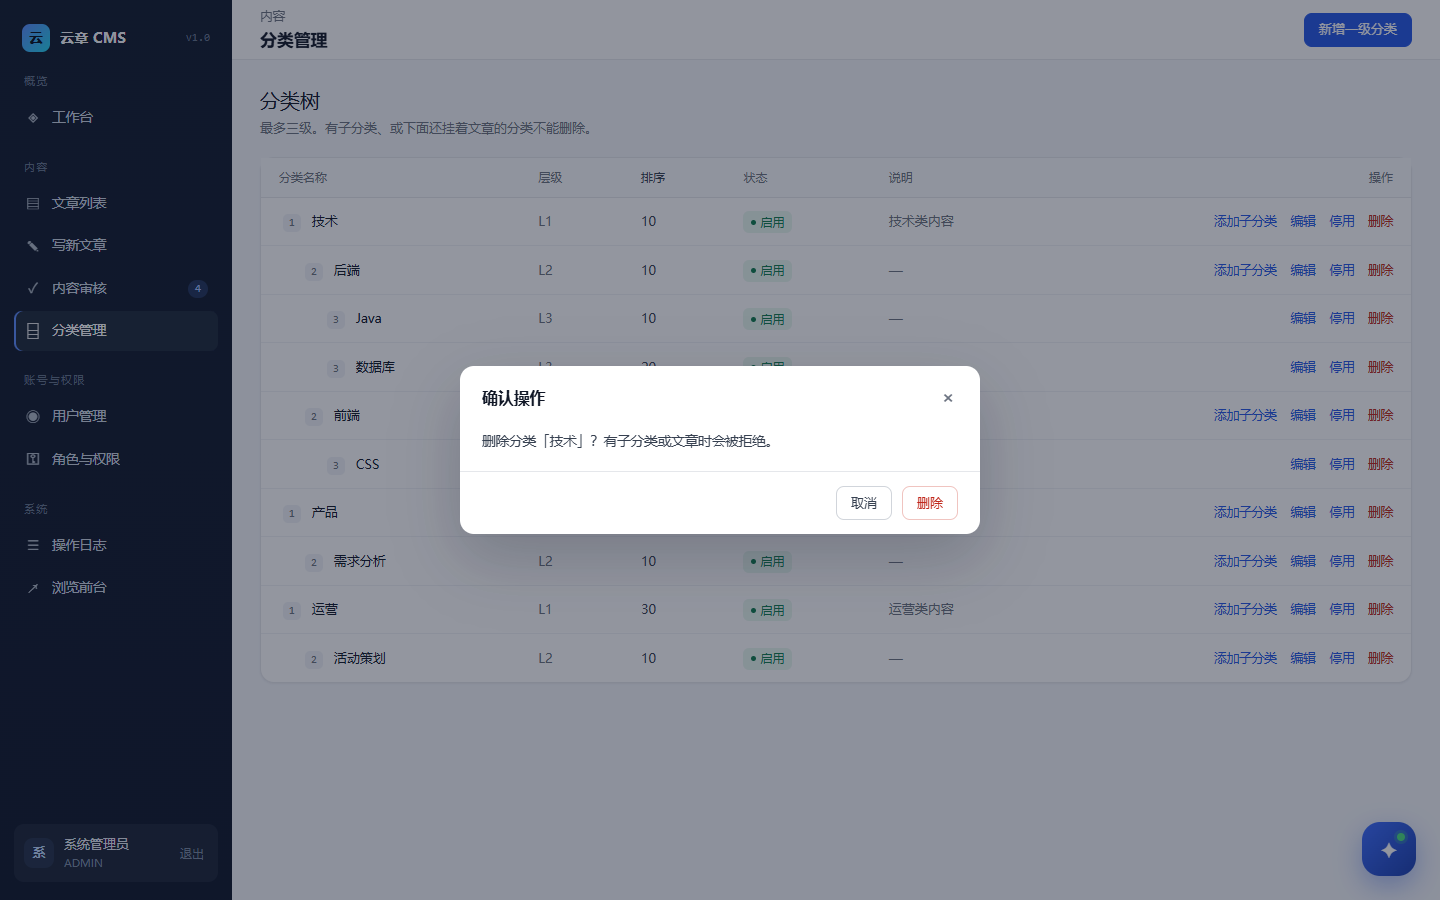
\includegraphics[width=\linewidth]{media/image24.png}

\subsubsection*{7.2.5 分类状态启停}\label{sec:cate-status}
\addcontentsline{toc}{subsubsection}{7.2.5 分类状态启停}

启停前检查是否还有启用的子分类，有则一并拒绝。

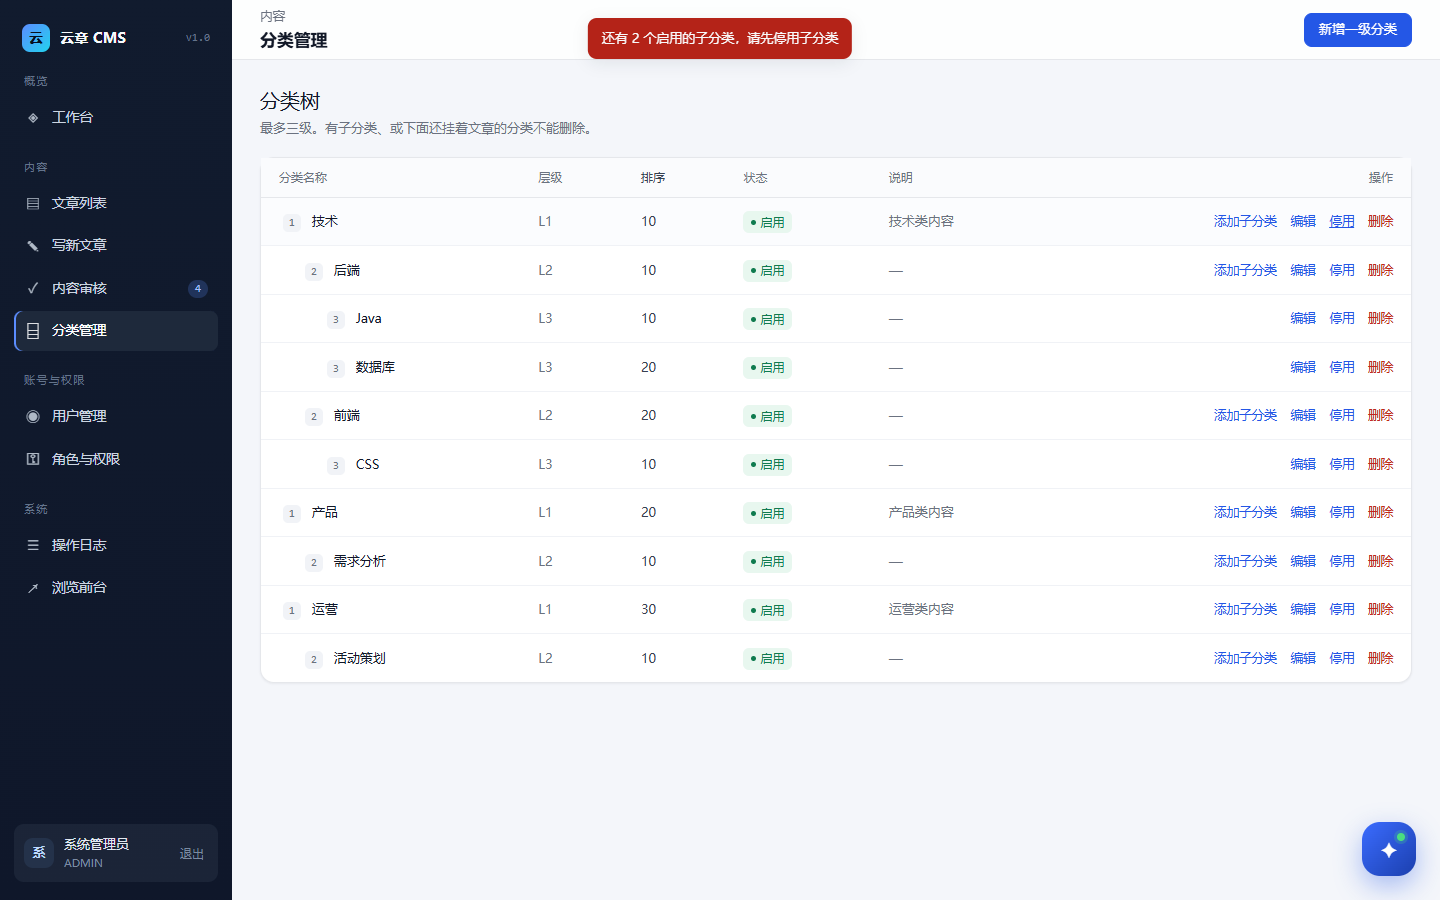
\includegraphics[width=\linewidth]{media/image25.png}

\subsubsection*{7.2.6 分类与内容关联绑定}\label{sec:cate-bind}
\addcontentsline{toc}{subsubsection}{7.2.6 分类与内容关联绑定}

文章通过 category\_id 外键绑定分类，分类删除前检查是否存在引用文章，有引用则拒绝删除，保证分类与内容关联的完整性。列表检索时按分类含子分类过滤，关联关系随分类树自动向下展开。

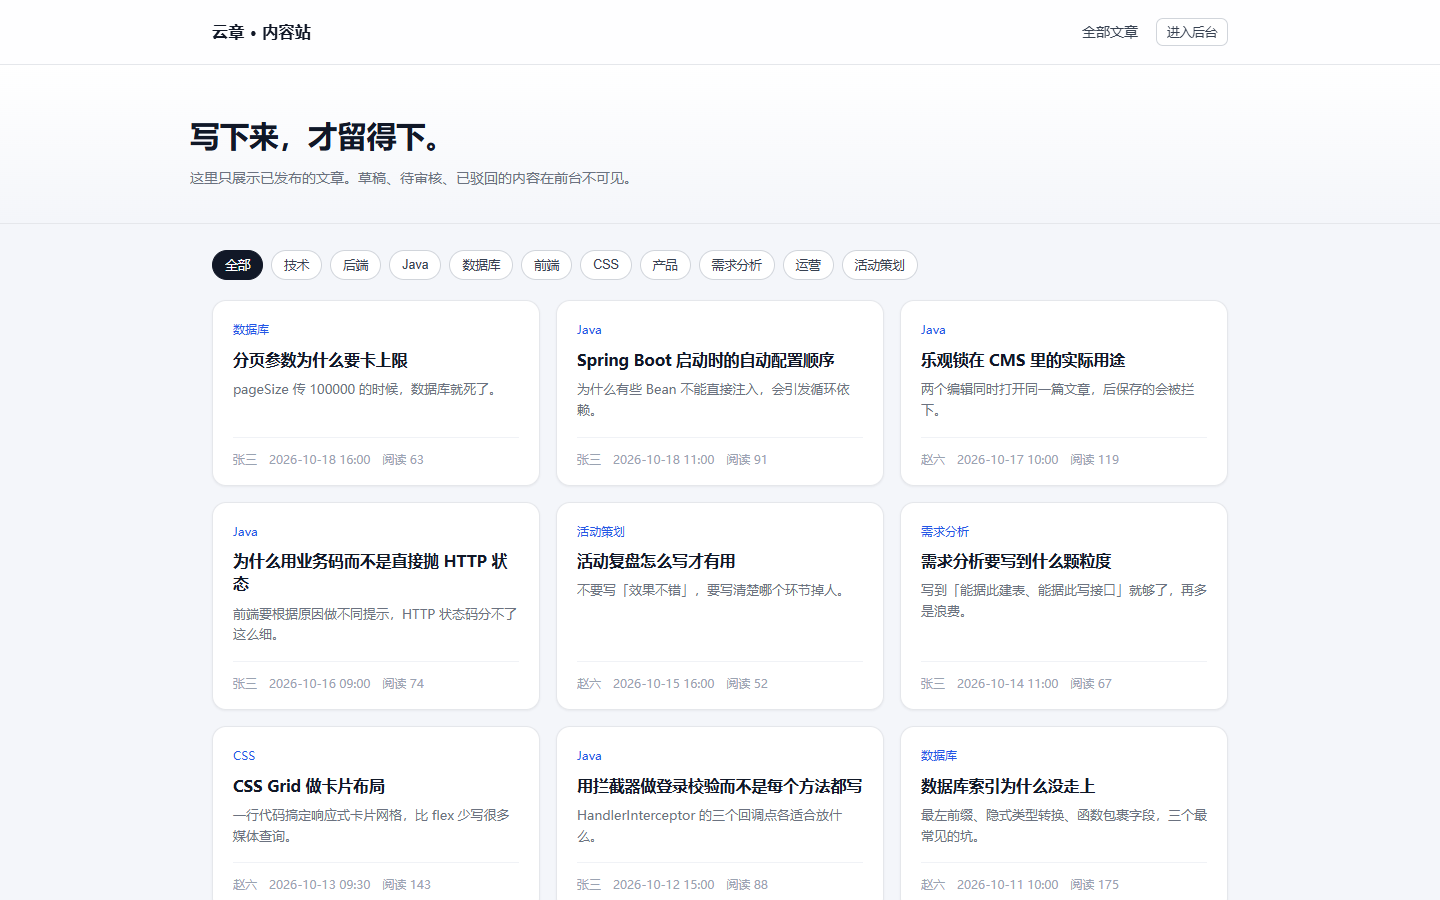
\includegraphics[width=\linewidth]{media/image26.png}

\subsection*{7.3 文章内容管理}\label{ux6587ux7ae0ux5185ux5bb9ux7ba1ux7406}
\addcontentsline{toc}{subsection}{7.3 文章内容管理}

按新增、编辑、批量发布、下架、删除、分页查询、多条件模糊检索、内容状态审核流程分述，各部分功能截屏如下。

本模块接口与功能说明如下表，驳回分支在 7.4 展开。

\begin{longtable}{@{}>{\raggedright\arraybackslash}p{8.4cm}>{\raggedright\arraybackslash}p{4.4cm}@{}}
\toprule
\textbf{接口名称} & \textbf{功能说明} \\
\midrule
\endfirsthead
\multicolumn{2}{@{}l}{\small（续表）}\\
\toprule
\textbf{接口名称} & \textbf{功能说明} \\
\midrule
\endhead
\multicolumn{2}{@{}l}{\textbf{文章} \quad /api/articles} \\
\midrule
GET /api/articles & 分页查询文章 \\
GET /api/articles/\{id\} & 查询文章详情 \\
POST /api/articles & 新建文章，保存为草稿 \\
PUT /api/articles/\{id\} & 修改草稿或驳回稿 \\
POST /api/articles/\{id\}/submit & 提交审核 \\
POST /api/articles/\{id\}/withdraw & 撤回文章回到草稿 \\
POST /api/articles/\{id\}/resubmit & 下架后重新提交审核 \\
POST /api/articles/\{id\}/approve & 审核通过并发布 \\
POST /api/articles/\{id\}/reject & 驳回文章 \\
POST /api/articles/\{id\}/offline & 下架文章 \\
POST /api/articles/batch/approve & 批量通过 \\
POST /api/articles/batch/offline & 批量下架 \\
DELETE /api/articles/\{id\} & 删除草稿或驳回稿 \\
\bottomrule
\end{longtable}

请求数据结构（DTO）直接取自代码。

\begin{verbatim}
public class ArticleSaveRequest {
    @NotBlank(message = "标题不能为空")
    @Size(max = 200, message = "标题最长 200 字")
    private String title;

    @Size(max = 500, message = "摘要最长 500 字")
    private String summary;

    @NotBlank(message = "正文不能为空")
    private String content;

    @NotNull(message = "请选择分类")
    private Long categoryId;

    private Integer version;   // 乐观锁版本号，编辑页回传
}

public class ArticleBatchRequest {
    @NotNull(message = "请选择文章")
    private List<Long> ids;

    private String opinion;    // 驳回必填
    private String reason;     // 下架必填
}
\end{verbatim}

文章状态主流转如下（完整五态七迁见 5.3）。

\begin{center}
\begin{tikzpicture}[
  node distance=5mm,
  box/.style={rectangle, draw, rounded corners=1pt, align=center, minimum width=5.8cm, minimum height=0.72cm, font=\small},
  arr/.style={-{Stealth}}
]
\node[box] (a) {草稿 DRAFT};
\node[box, below=of a] (b) {提交 submit 进入待审核 PENDING};
\node[box, below=of b] (c) {审核通过 approve 进入已发布 PUBLISHED};
\node[box, below=of c] (d) {下架 offline 进入已下架 OFFLINE};
\node[box, below=of d] (e) {重提 resubmit 再次进入 PENDING};
\draw[arr] (a) -- (b);
\draw[arr] (b) -- (c);
\draw[arr] (c) -- (d);
\draw[arr] (d) -- (e);
\end{tikzpicture}
\end{center}

\subsubsection*{7.3.1 内容新增}\label{sec:art-add}
\addcontentsline{toc}{subsubsection}{7.3.1 内容新增}

新增文章时一律保存为 DRAFT，不允许创建即发布。

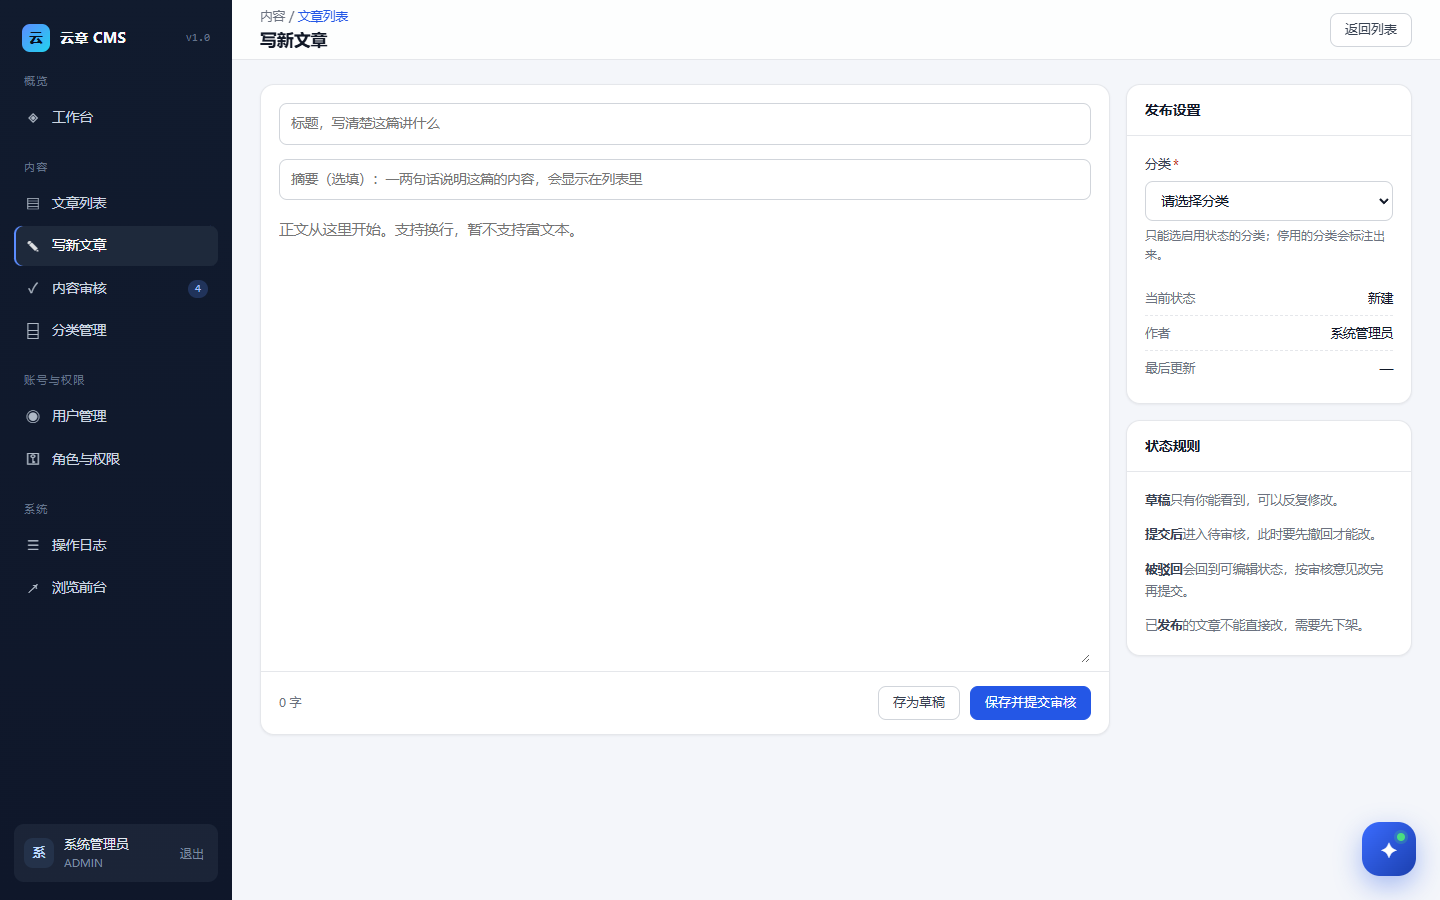
\includegraphics[width=\linewidth]{media/image27.png}

\subsubsection*{7.3.2 内容编辑}\label{sec:art-edit}
\addcontentsline{toc}{subsubsection}{7.3.2 内容编辑}

编辑只允许 DRAFT 与 REJECTED 两种状态，并带 version 乐观锁，版本不符返回 40900。

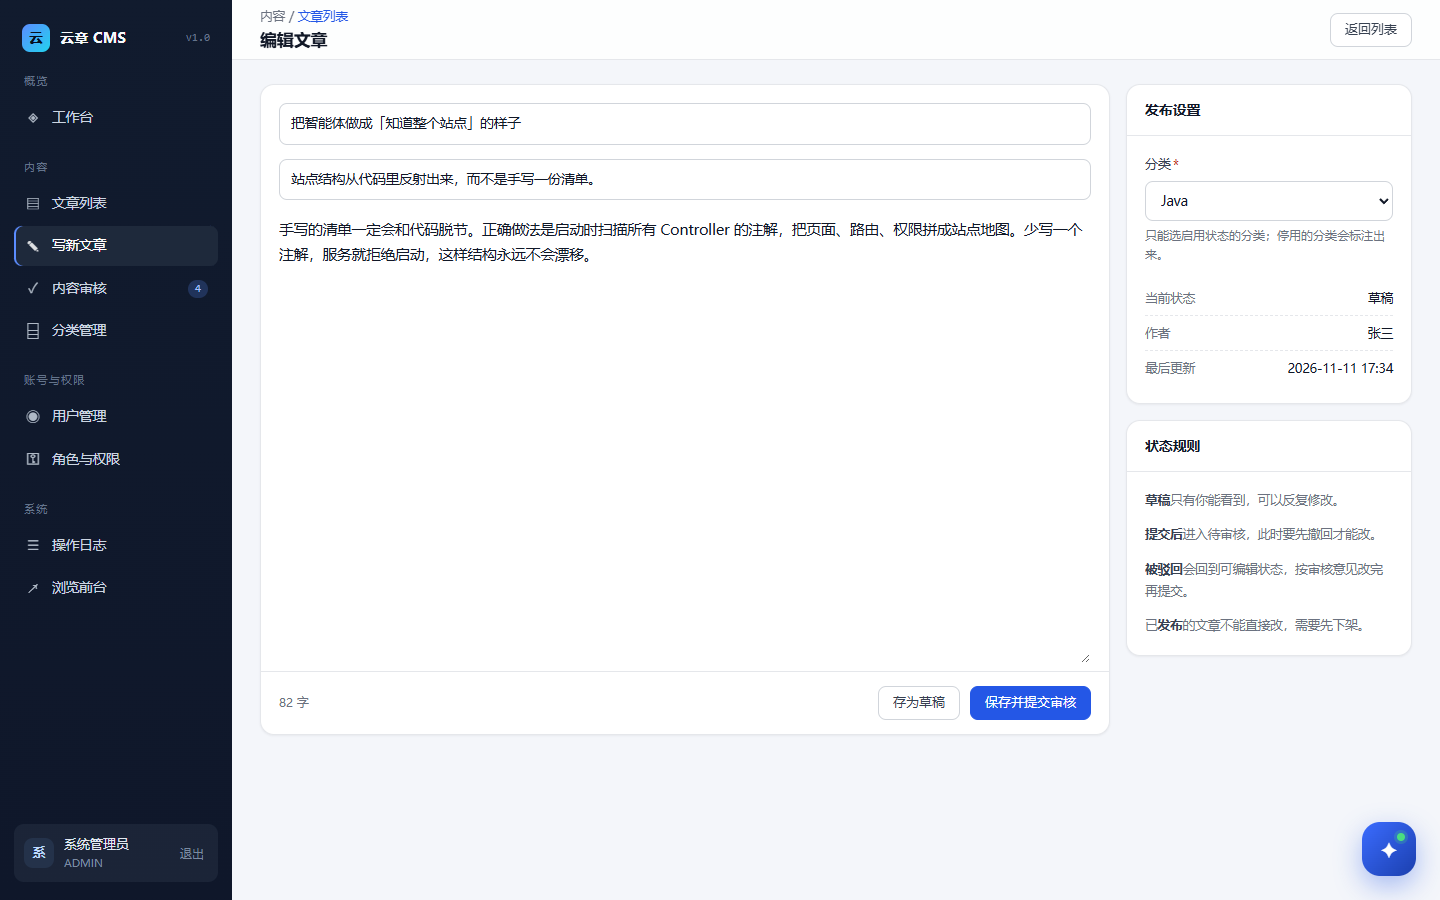
\includegraphics[width=\linewidth]{media/image28.png}

\subsubsection*{7.3.3 批量发布}\label{sec:art-publish}
\addcontentsline{toc}{subsubsection}{7.3.3 批量发布}

批量发布由 POST /api/articles/batch/approve 完成，逐条处理，不做整体事务。一条数据状态不对，不应该让另外 99 条白做。返回结构固定为 total、success、failed、reasons 四个字段，失败原因逐条可见。

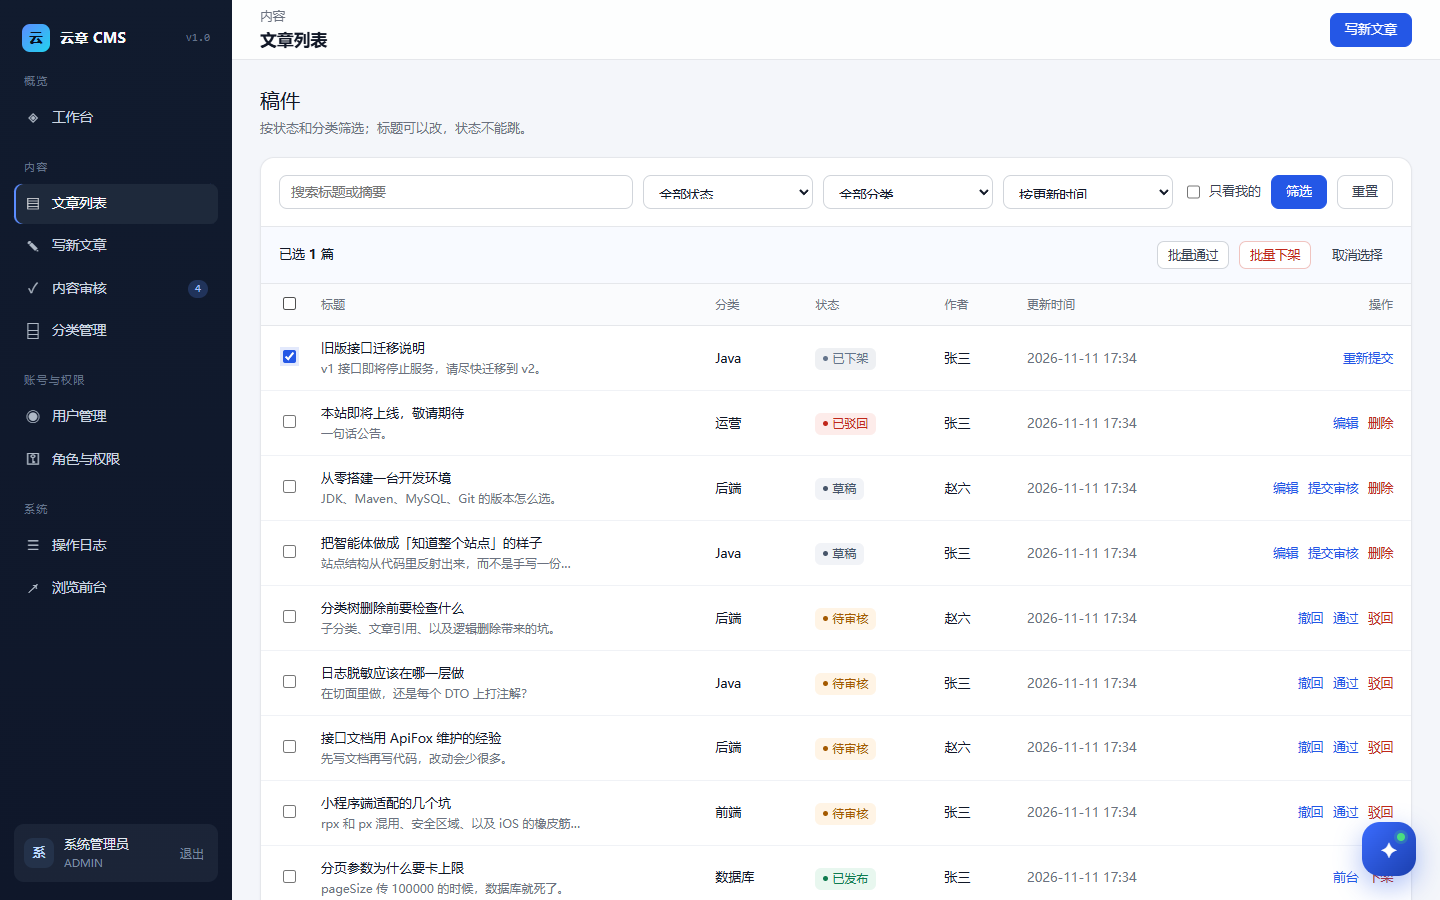
\includegraphics[width=\linewidth]{media/image29.png}

\subsubsection*{7.3.4 下架}\label{sec:art-offline}
\addcontentsline{toc}{subsubsection}{7.3.4 下架}

下架由 POST /api/articles/batch/offline 完成，同样逐条处理，失败明细可追溯。

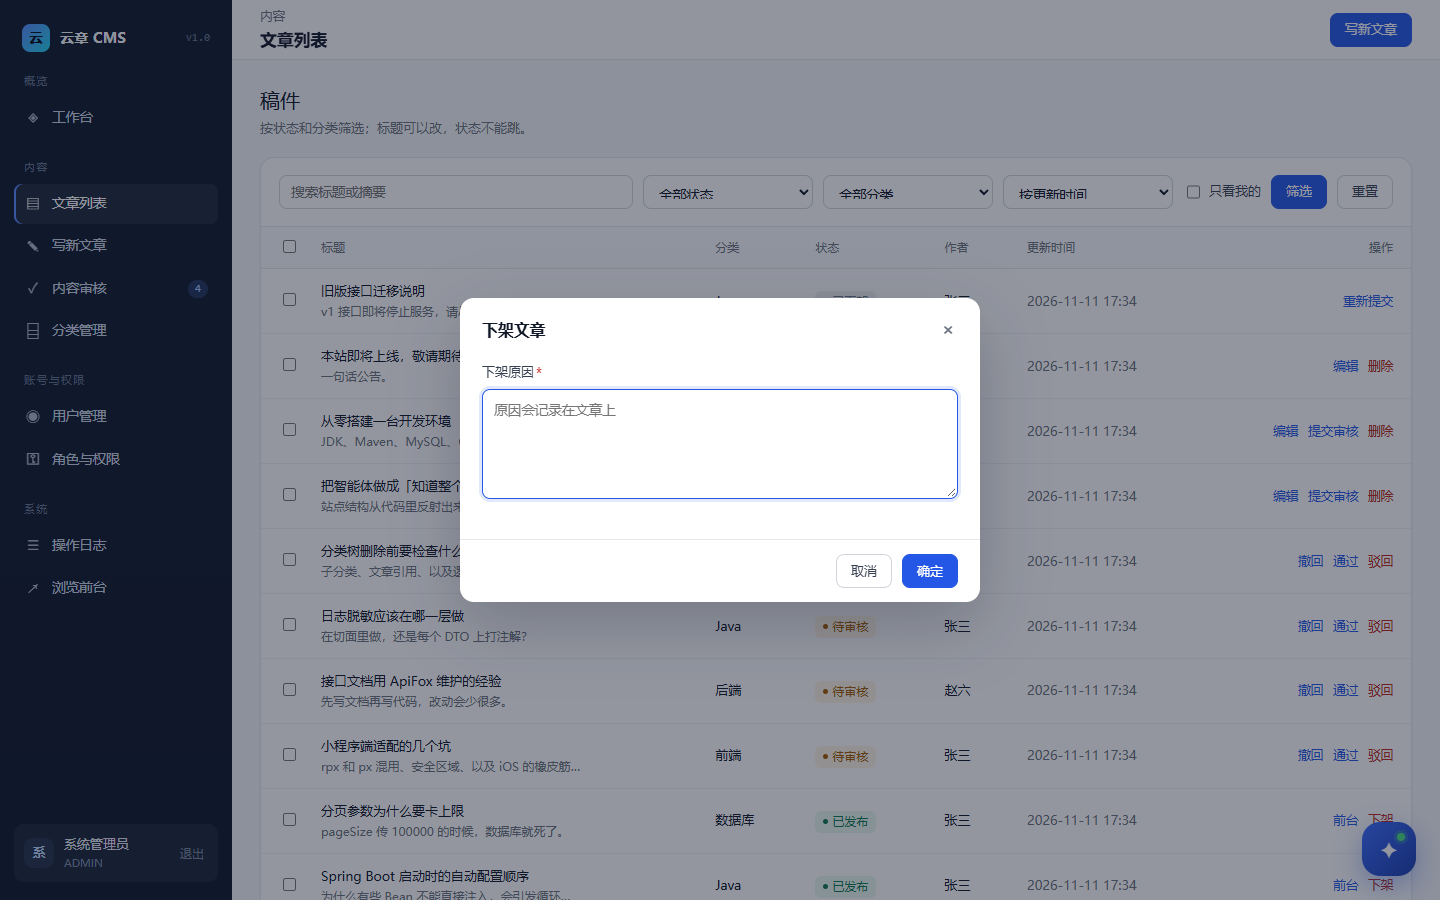
\includegraphics[width=\linewidth]{media/image30.png}

\subsubsection*{7.3.5 删除}\label{sec:art-del}
\addcontentsline{toc}{subsubsection}{7.3.5 删除}

删除仅限 DRAFT 与 REJECTED 两种状态，采用逻辑删除，引用关系保持。

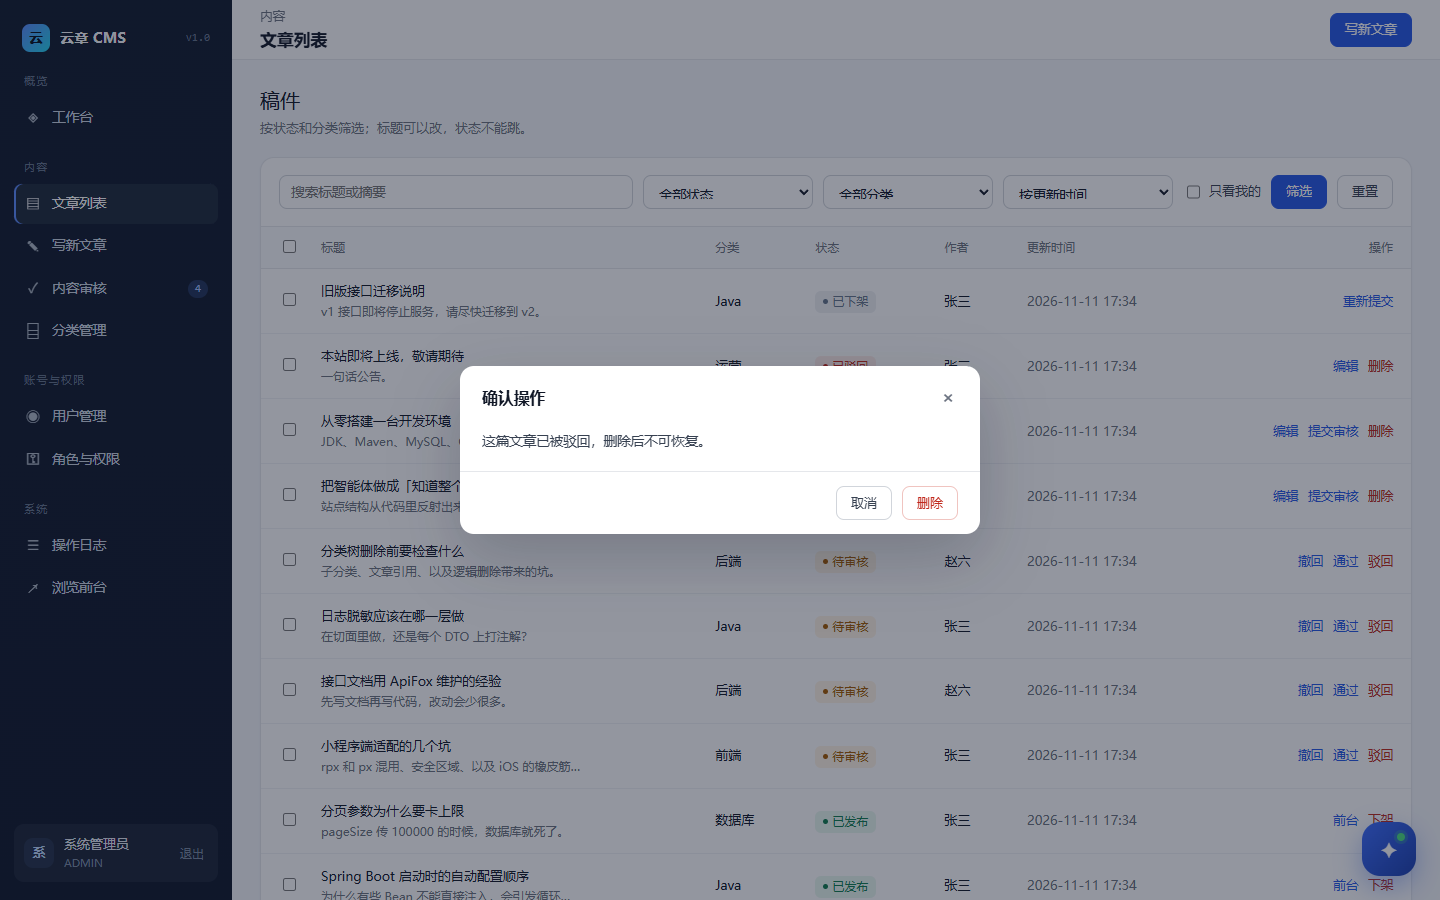
\includegraphics[width=\linewidth]{media/image31.png}

\subsubsection*{7.3.6 分页查询}\label{sec:art-page}
\addcontentsline{toc}{subsubsection}{7.3.6 分页查询}

分页用 MP 的 PaginationInnerInterceptor 实现，maxLimit 设为 200，在插件层兜底防止拉全表，详见 8.1。

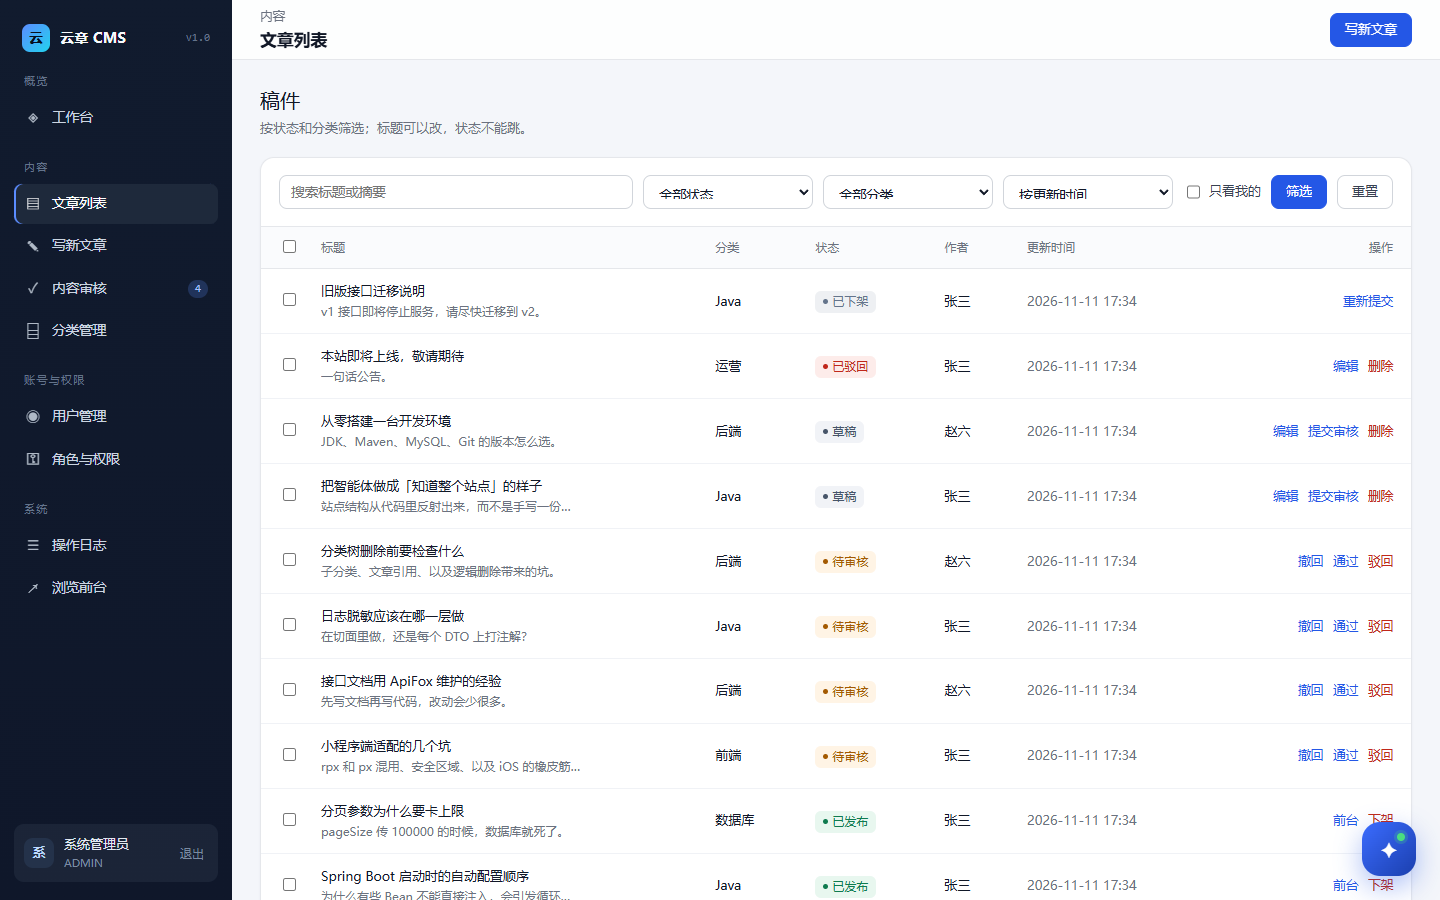
\includegraphics[width=\linewidth]{media/image32.png}

\subsubsection*{7.3.7 多条件模糊检索}\label{sec:art-search}
\addcontentsline{toc}{subsubsection}{7.3.7 多条件模糊检索}

列表支持关键词、分类含子分类、状态、作者、仅看我的组合筛选，配合多维排序与分页，详见 8.1 与 8.3。

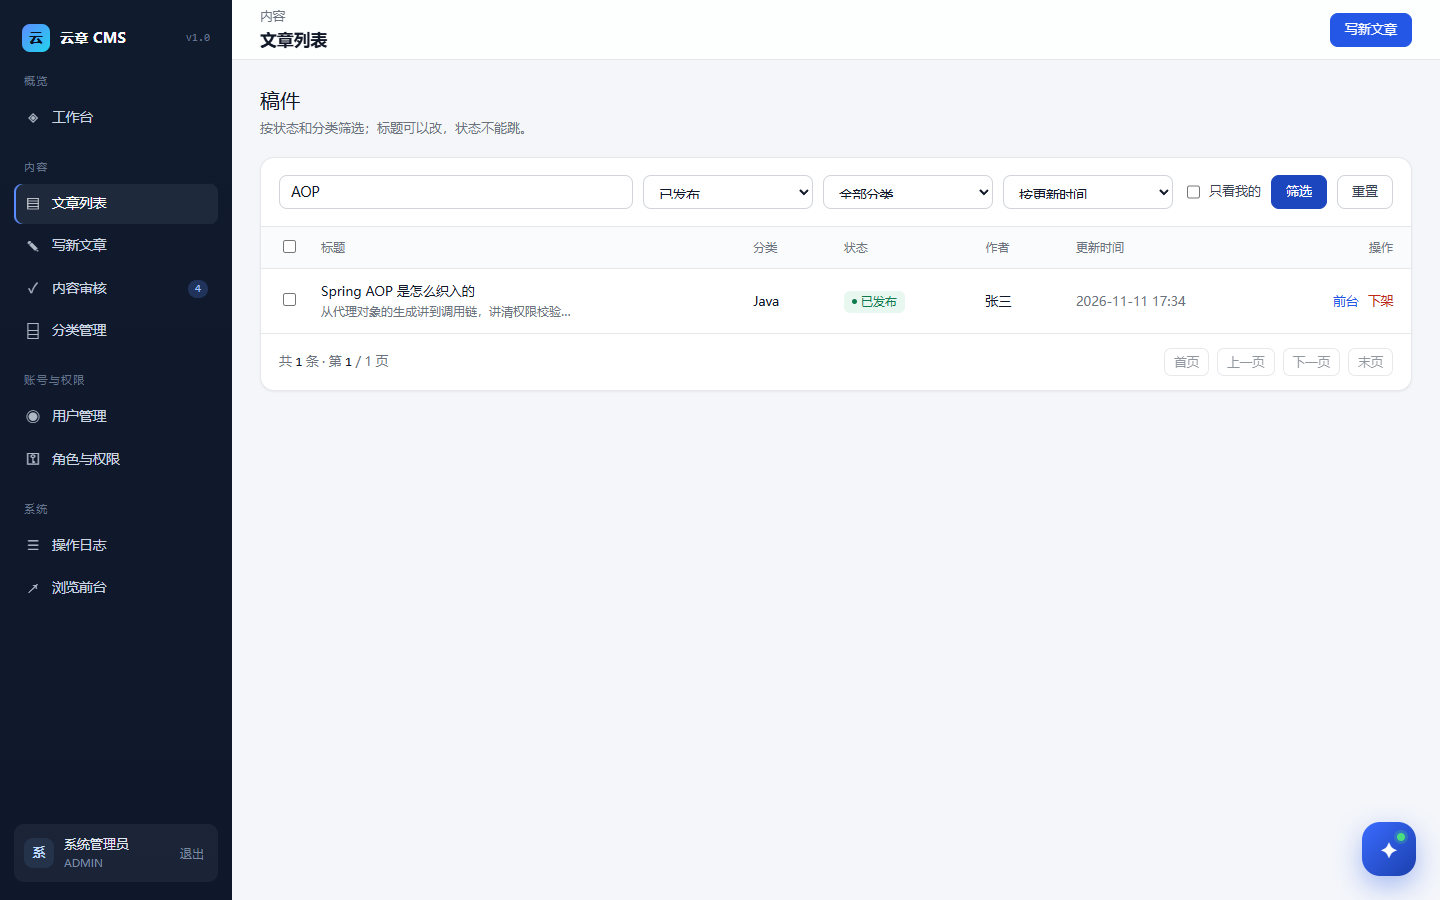
\includegraphics[width=\linewidth]{media/image33.png}

\subsubsection*{7.3.8 内容状态审核流程}\label{sec:art-audit}
\addcontentsline{toc}{subsubsection}{7.3.8 内容状态审核流程}

提交、撤回、重提全部走 ArticleStateMachine.next()，不在 Service 里写状态判断。审核动作只有通过与驳回两个入口，详细规则与职责分离见 7.4。

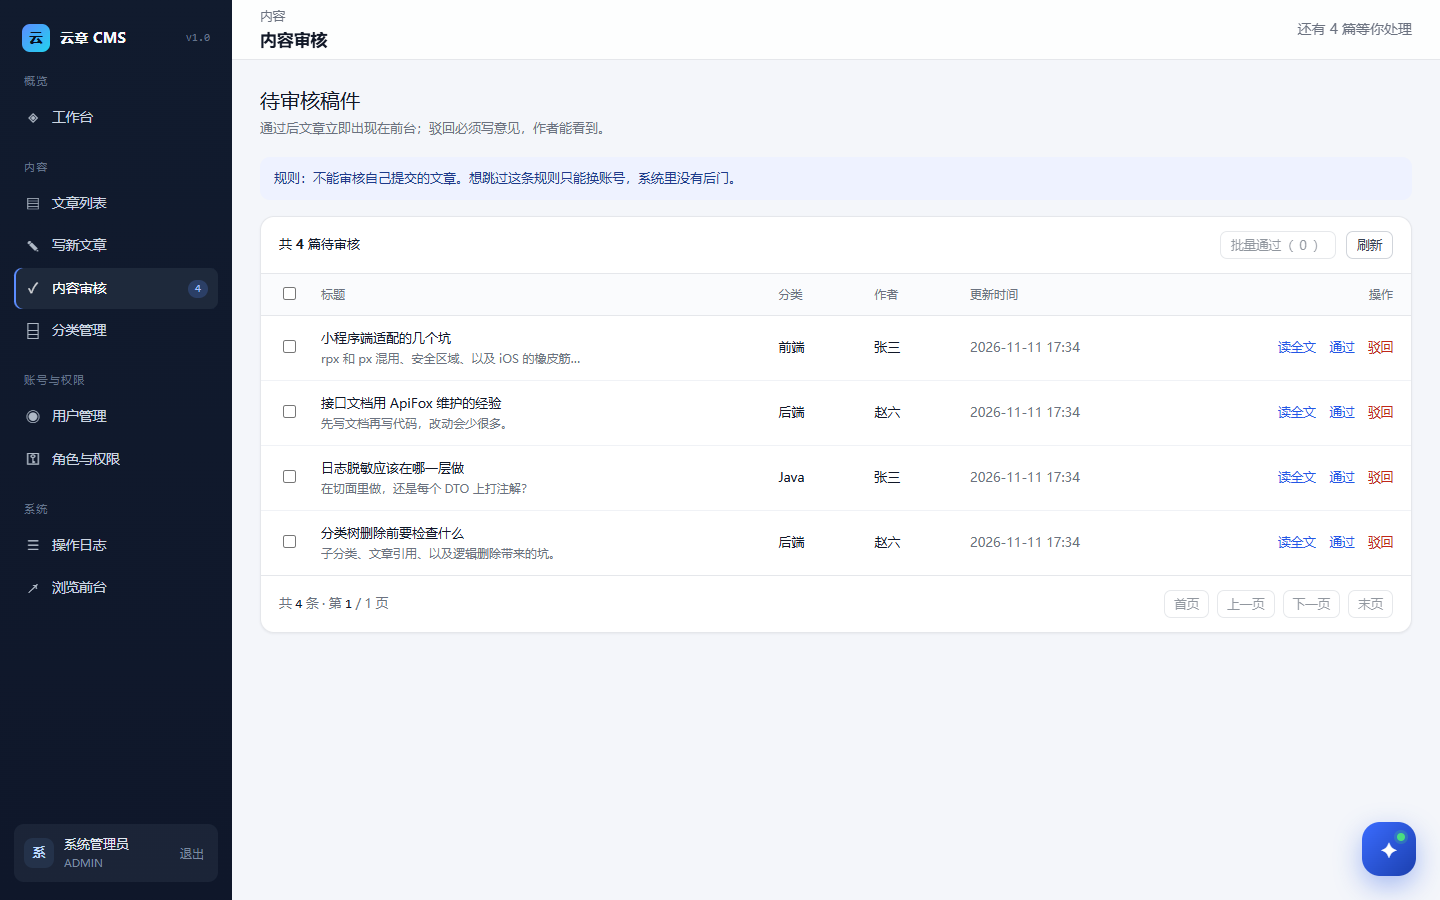
\includegraphics[width=\linewidth]{media/image34.png}

\subsection*{7.4 内容审核流程}\label{ux5185ux5bb9ux5ba1ux6838ux6d41ux7a0b}
\addcontentsline{toc}{subsection}{7.4 内容审核流程}

审核动作只有两个入口，即通过 APPROVE 和驳回 REJECT，两者都要求当前状态为 PENDING。

驳回意见必填，ArticleBatchRequest.opinion 用 @NotBlank 校验，空意见直接返回 40000。

不能审核自己的稿，Service 里比对 article.authorId 与当前审核员 id，相同则拒绝，实现职责分离。

审核全程留痕。通过时写 auditor\_id、audit\_time、publish\_time，驳回时写 auditor\_id、audit\_time、audit\_opinion。

从作者视角看，被驳回的稿件在被驳回卡片里可见。作者修改后执行 MODIFY 回到 DRAFT，再次提交就回到审核队列。

批量通过与批量下架复用单条逻辑，失败明细可追溯。

\subsection*{7.5 系统基础运维}\label{ux7cfbux7edfux57faux7840ux8fd0ux7ef4}
\addcontentsline{toc}{subsection}{7.5 系统基础运维}

以下按操作日志记录、数据安全防护、异常统一处理、请求参数校验分述，各部分功能截屏如下。

本模块接口与功能说明如下表。

\begin{longtable}{@{}>{\raggedright\arraybackslash}p{8.4cm}>{\raggedright\arraybackslash}p{4.4cm}@{}}
\toprule
\textbf{接口名称} & \textbf{功能说明} \\
\midrule
\endfirsthead
\multicolumn{2}{@{}l}{\small（续表）}\\
\toprule
\textbf{接口名称} & \textbf{功能说明} \\
\midrule
\endhead
\multicolumn{2}{@{}l}{\textbf{日志} \quad /api/logs} \\
\midrule
GET /api/logs & 分页查询操作日志 \\
\multicolumn{2}{@{}l}{\textbf{工作台} \quad /api/dashboard} \\
\midrule
GET /api/dashboard/stats & 查询工作台统计 \\
\bottomrule
\end{longtable}

异常统一处理流程如下。

\begin{center}
\begin{tikzpicture}[
  node distance=5mm,
  box/.style={rectangle, draw, rounded corners=1pt, align=center, minimum width=5.6cm, minimum height=0.72cm, font=\small},
  arr/.style={-{Stealth}}
]
\node[box] (a) {控制器或服务层抛出异常};
\node[box, below=of a] (b) {GlobalExceptionHandler 统一捕获};
\node[box, below=of b] (c) {按类型分派：BizException / 校验异常 / 未捕获};
\node[box, below=of c] (d) {转统一 Result，带业务码与 traceId};
\draw[arr] (a) -- (b);
\draw[arr] (b) -- (c);
\draw[arr] (c) -- (d);
\end{tikzpicture}
\end{center}

\subsubsection*{7.5.1 操作日志记录}\label{sec:oplog}
\addcontentsline{toc}{subsubsection}{7.5.1 操作日志记录}

操作日志由 @OperLog 标注写接口，LogAspect 记录谁、何时、调了什么、脱敏后的参数、结果、耗时、IP 和 traceId。结果分三类，SUCCESS 表示成功，DENIED 表示被权限切面拦截，FAIL 表示业务异常或未捕获异常。切面顺序保证 DENIED 不会被内层异常吞掉。

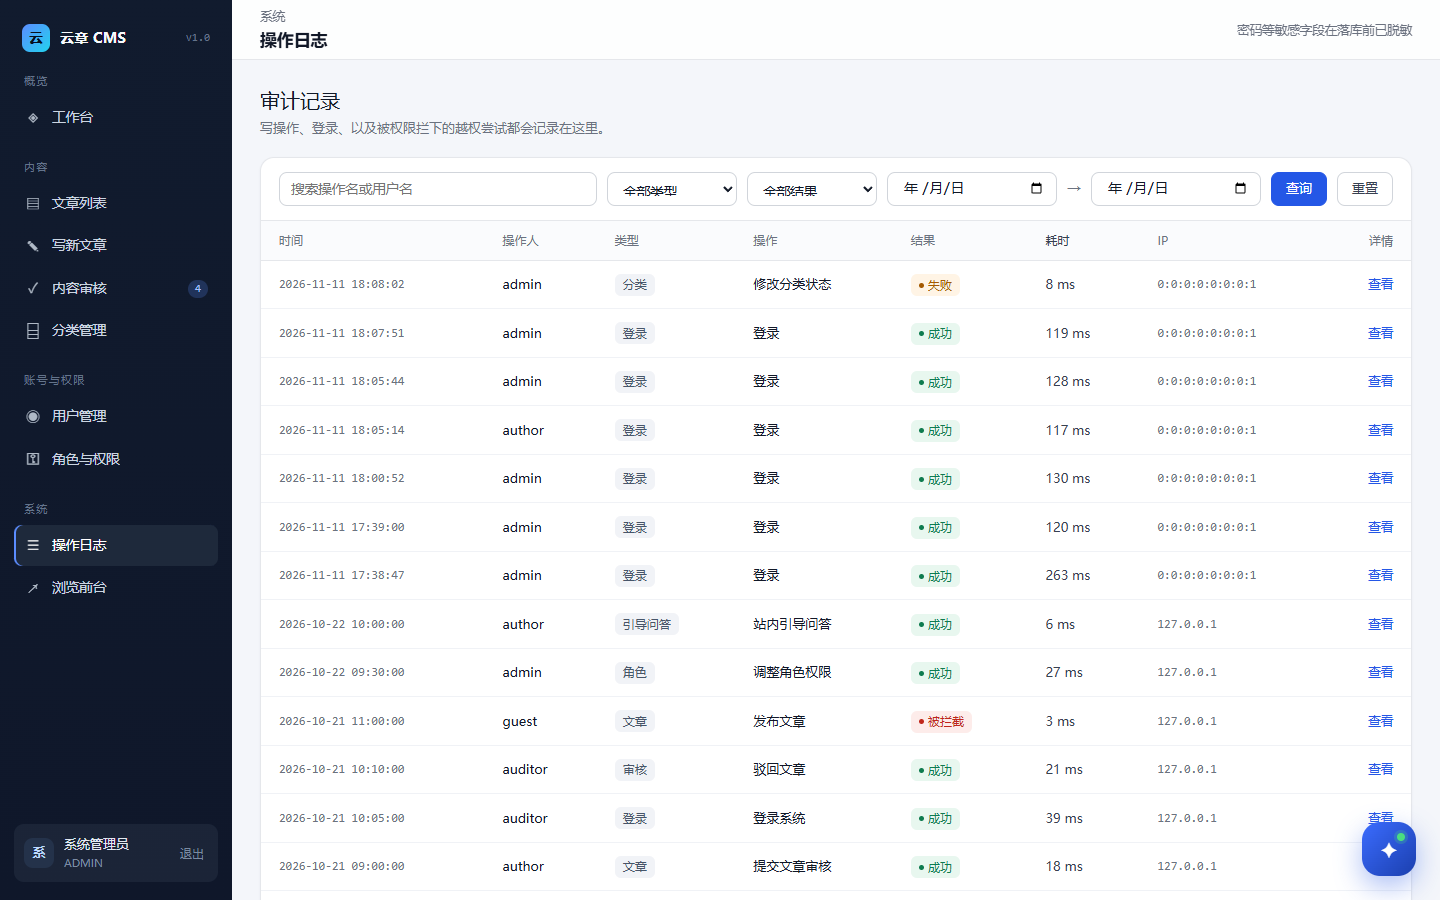
\includegraphics[width=\linewidth]{media/image35.png}

\subsubsection*{7.5.2 数据安全防护}\label{sec:datasec}
\addcontentsline{toc}{subsubsection}{7.5.2 数据安全防护}

数据安全防护有四条。密码用 BCrypt 单向加密，日志中 password、token、apiKey 等字段按名脱敏。入参按内容二次打码，正文里的手机号、身份证号、银行卡号写库前替换为掩码形态。敏感信息提交拦截由 SensitiveInfoDetector 完成，检测身份证、手机号、银行卡、邮箱、API key、明文口令六类，规则只在后端一份。前端保存前调用 POST /api/articles/sensitive-check 弹提示框，后端 create 和 update 用同规则硬拦，绕过前端也返回 40003。未捕获异常只回通用文案 50000，堆栈仅进服务端日志，不随响应外泄。

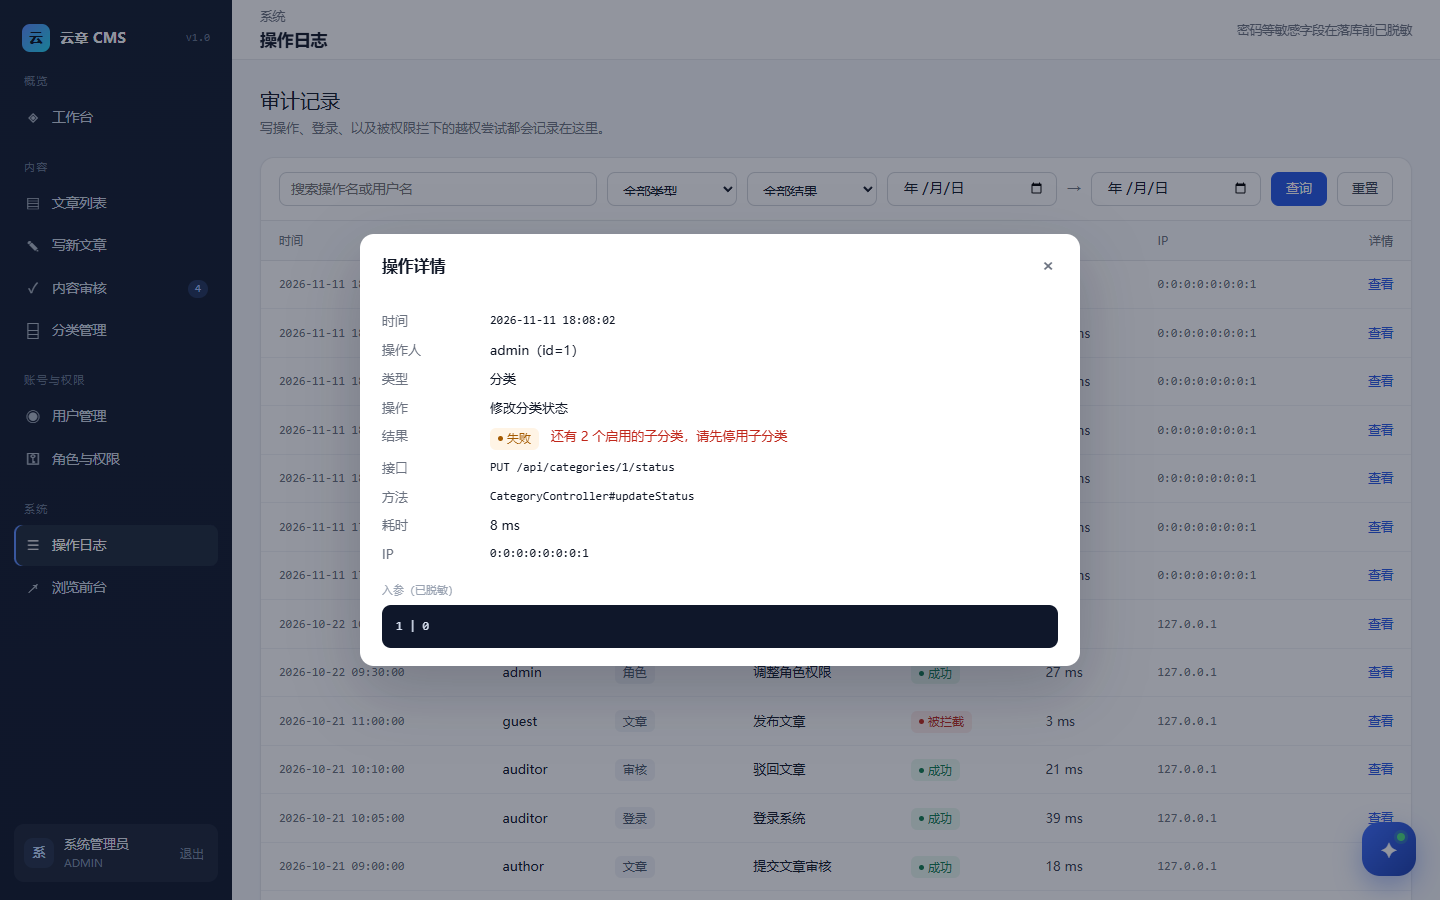
\includegraphics[width=\linewidth]{media/image36.png}

\subsubsection*{7.5.3 异常统一处理}\label{sec:excep}
\addcontentsline{toc}{subsubsection}{7.5.3 异常统一处理}

异常统一处理由 GlobalExceptionHandler 完成，把 BizException、参数校验异常、未捕获异常统一转成 Result 结果。BizException 带业务码，参数校验异常返回 40000，未捕获异常返回 50000，并携带 traceId 方便对日志。

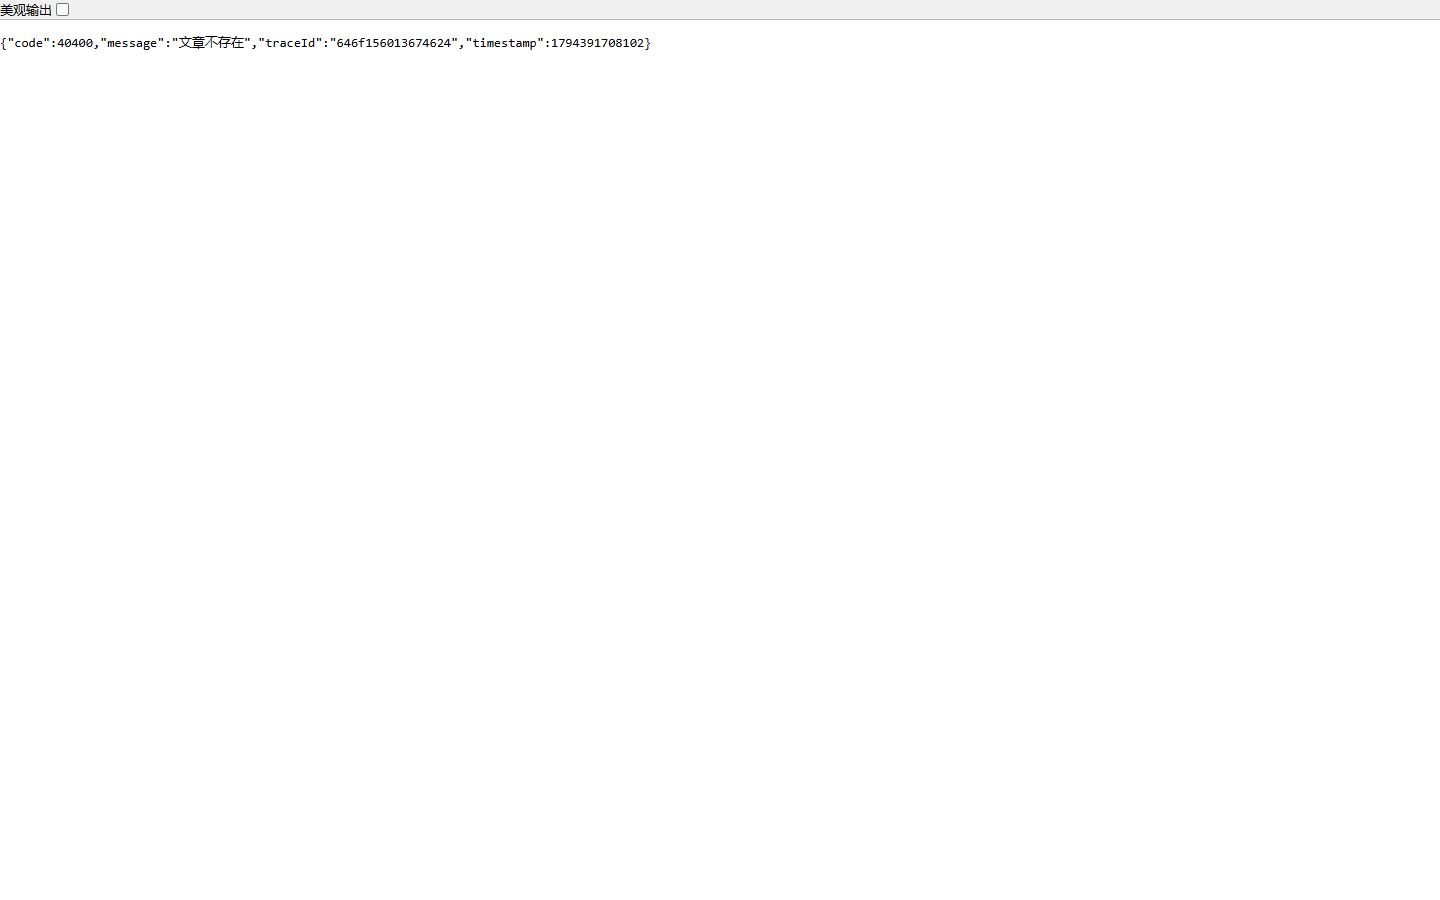
\includegraphics[width=\linewidth]{media/image37.png}

\subsubsection*{7.5.4 请求参数校验}\label{sec:valid}
\addcontentsline{toc}{subsubsection}{7.5.4 请求参数校验}

请求参数校验在 DTO 上使用 @NotBlank、@Size、@Pattern、@Email，控制器方法参数加 @Valid，校验失败由全局处理器统一转码。

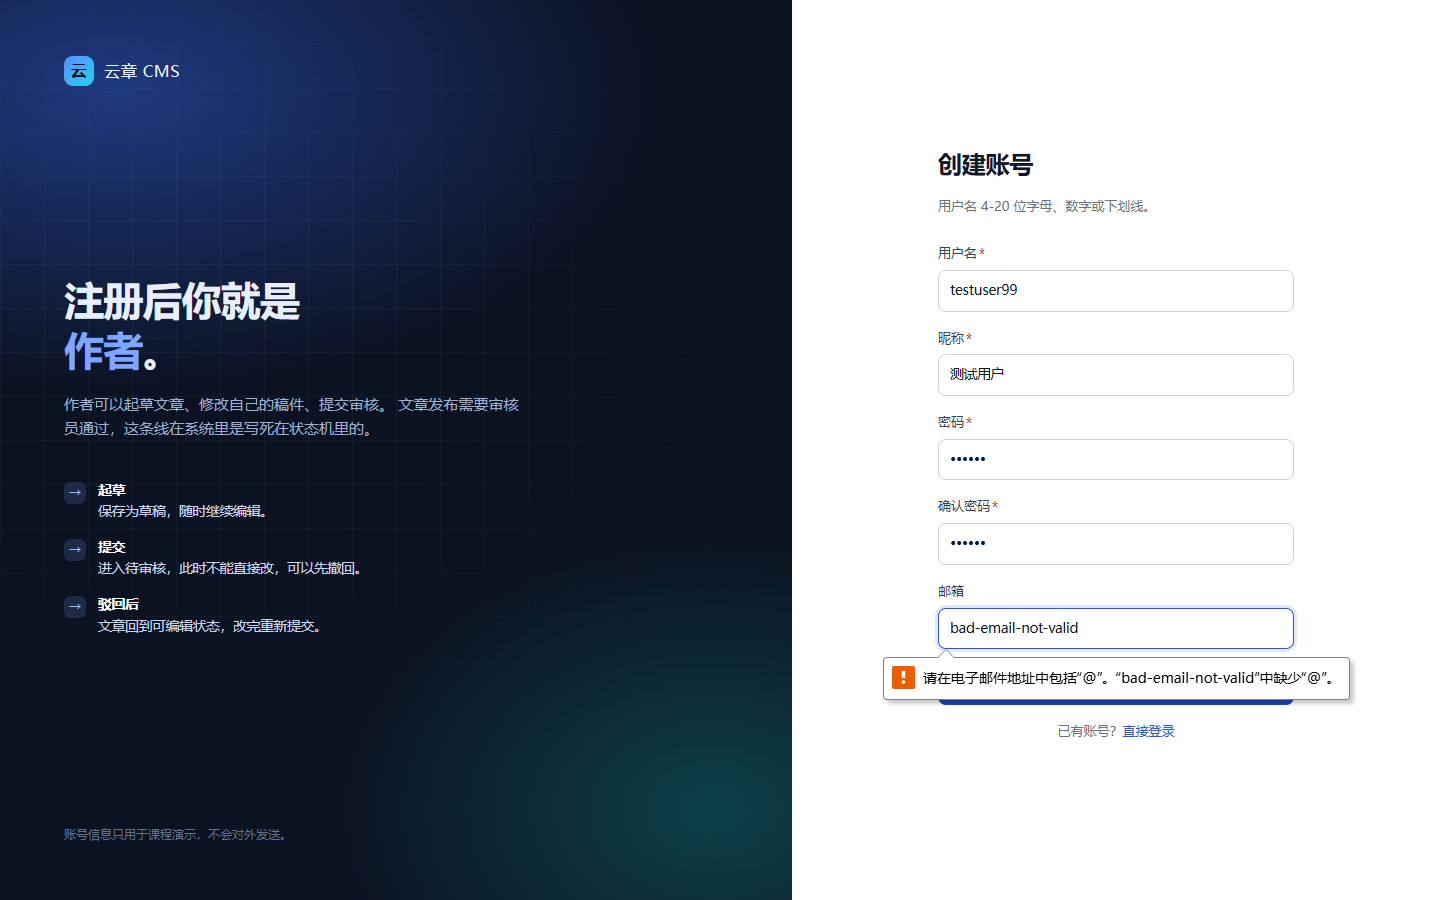
\includegraphics[width=\linewidth]{media/image38.png}

\section*{八、进阶拓展功能}\label{sec:advanced-features}
\addcontentsline{toc}{section}{八、进阶拓展功能}



\subsection*{8.1 高级数据处理}\label{ux9ad8ux7ea7ux6570ux636eux5904ux7406}
\addcontentsline{toc}{subsection}{8.1 高级数据处理}

本章覆盖分页、排序、批量、逻辑删除、自动填充五个数据层特性，逐个小节展开，每个小节配一张功能截屏。

\subsubsection*{8.1.1 分页高级查询}\label{sec:page}
\addcontentsline{toc}{subsubsection}{8.1.1 分页高级查询}

分页用 MP 的 PaginationInnerInterceptor 实现，maxLimit 设为 200，在插件层兜底，防止绕过 Service 校验的请求拉全表。分页结果统一包装成 PageResult，返回总数与当前页。

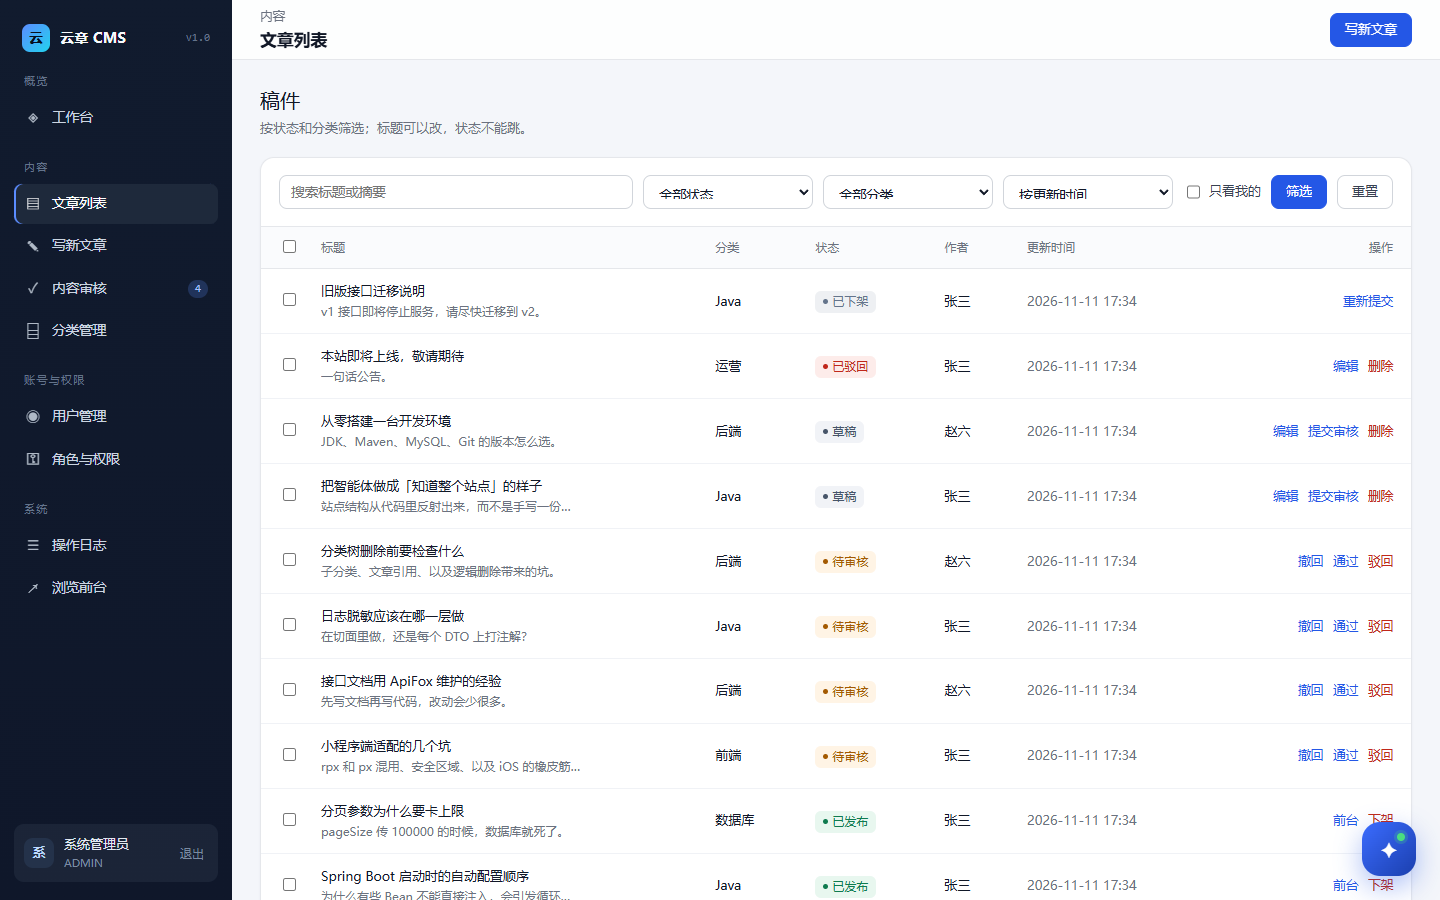
\includegraphics[width=\linewidth]{media/image39.png}

\subsubsection*{8.1.2 多维排序筛选}\label{sec:sort}
\addcontentsline{toc}{subsubsection}{8.1.2 多维排序筛选}

多维排序用 SortWhitelist 实现，入参形如 createTime,desc、title,asc，逻辑名映射物理列，最多 3 个字段，可追加唯一键做 tiebreaker，避免翻页重复或漏行。

SortWhitelist 值得单独说明：ORDER BY 后面不能使用预编译占位符，直接把前端传的字段拼进去就是注入入口。解决办法是只允许映射表命中项通过，非法字段抛 40000 并列出可选值。物理列名\textbf{永远不会来自客户端}。

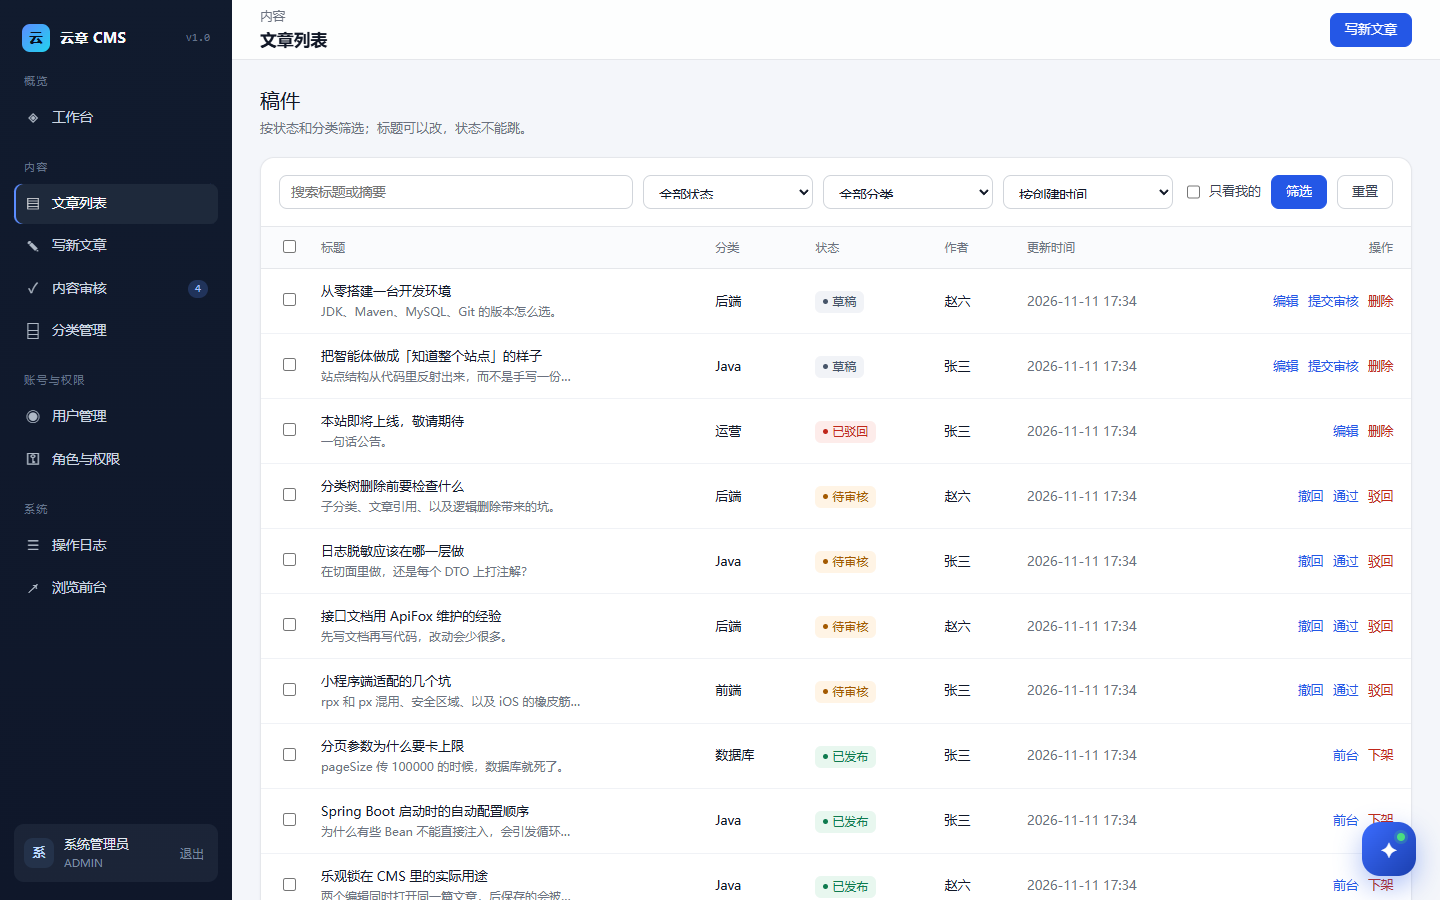
\includegraphics[width=\linewidth]{media/image40.png}

\subsubsection*{8.1.3 批量处理}\label{sec:batch}
\addcontentsline{toc}{subsubsection}{8.1.3 批量处理}

批量处理由 ArticleService.batchApprove 与 batchOffline 实现，逐条容错，返回成功数与失败明细。

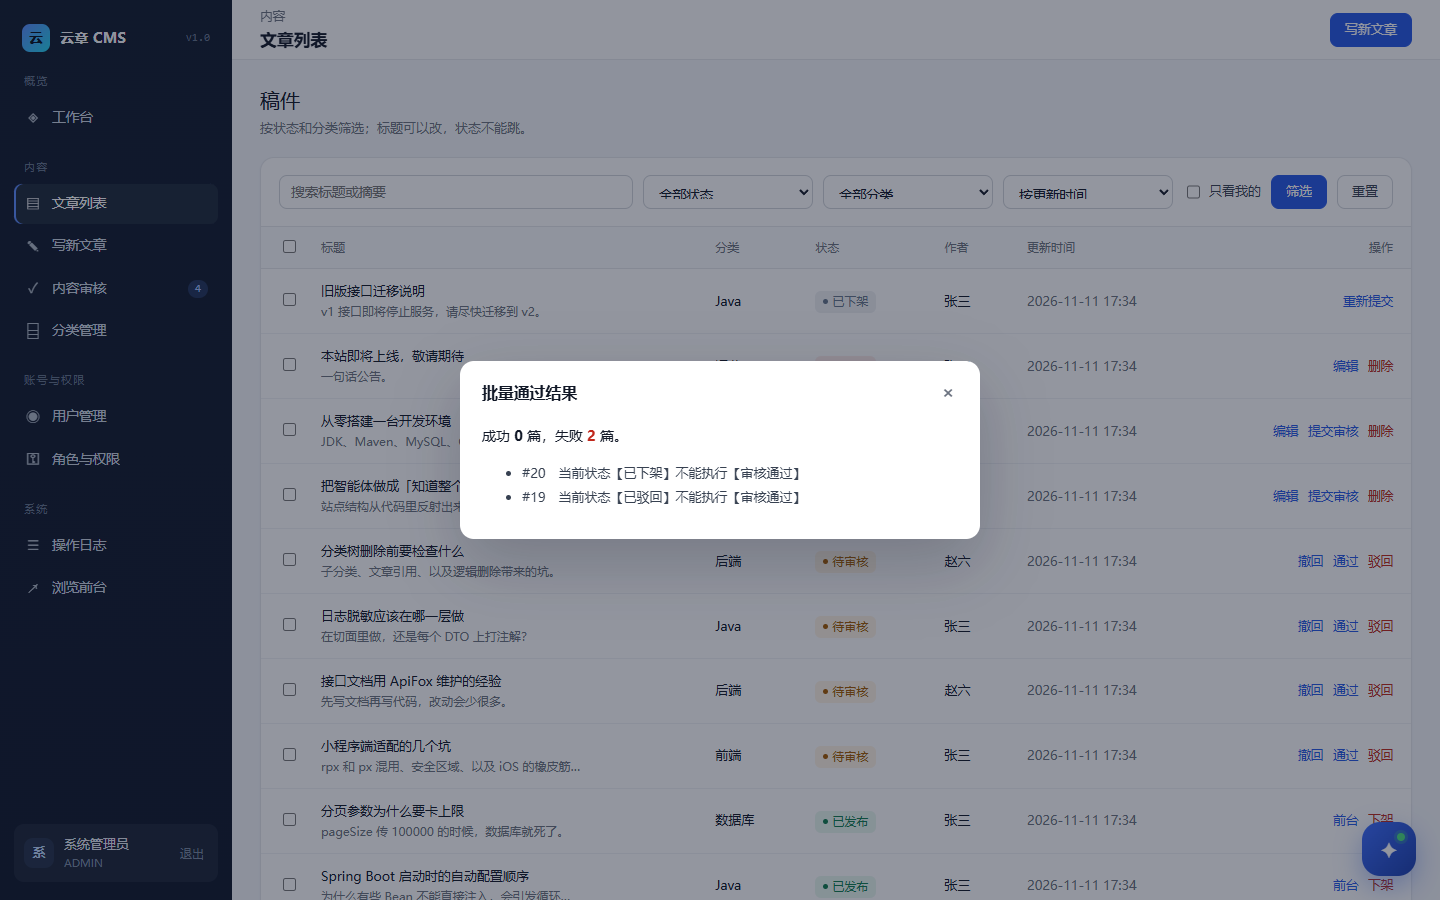
\includegraphics[width=\linewidth]{media/image41.png}

\subsubsection*{8.1.4 逻辑删除}\label{sec:logic-del}
\addcontentsline{toc}{subsubsection}{8.1.4 逻辑删除}

逻辑删除用 @TableLogic 加 deleted 字段实现，全局配置 logic-delete-field 为 deleted，业务代码不写 deleted = 0。删除后数据仍在库里，可恢复。

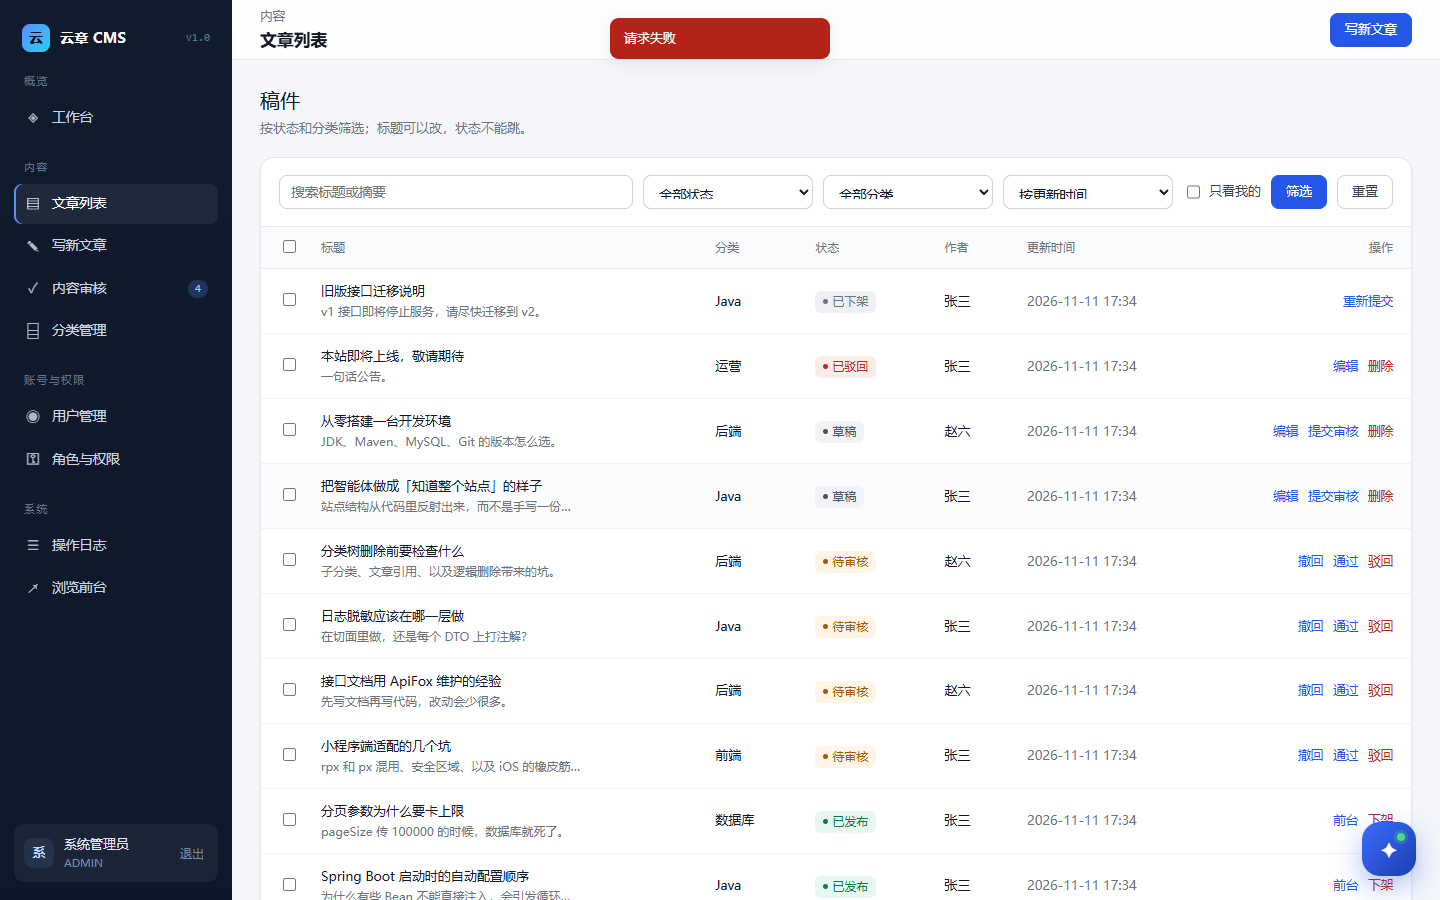
\includegraphics[width=\linewidth]{media/image42.png}

\subsubsection*{8.1.5 数据自动填充}\label{sec:autofill}
\addcontentsline{toc}{subsubsection}{8.1.5 数据自动填充}

数据自动填充用 AuditMetaObjectHandler 实现，createTime、updateTime、createBy、updateBy 由拦截器写入，业务代码不手写。

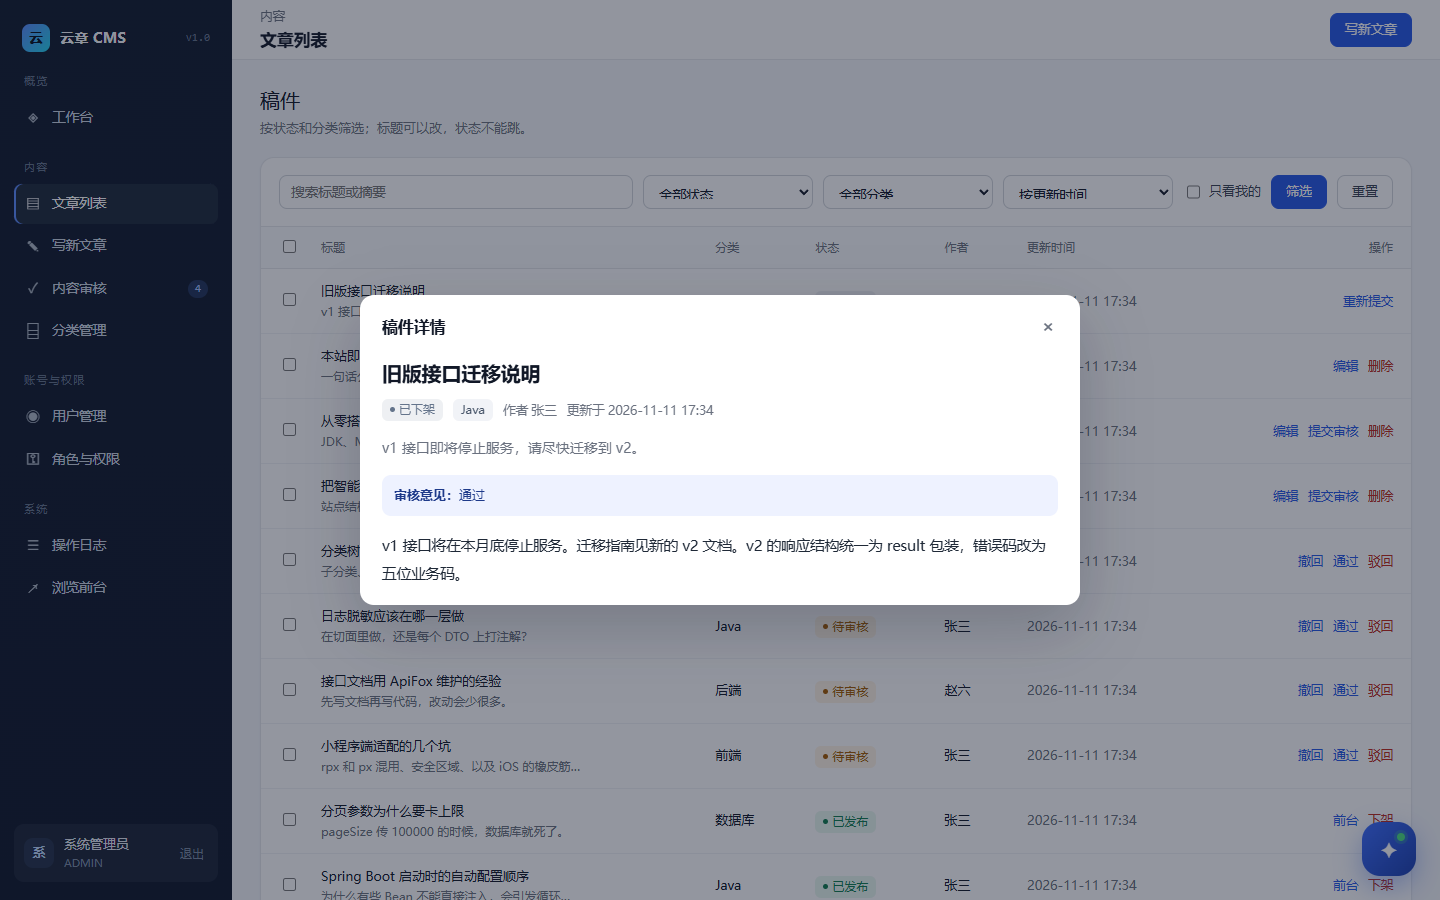
\includegraphics[width=\linewidth]{media/image43.png}

\subsection*{8.2 MyBatis-Plus 高级特性整合}\label{mybatis-plus-ux9ad8ux7ea7ux7279ux6027ux6574ux5408}
\addcontentsline{toc}{subsection}{8.2 MyBatis-Plus 高级特性整合}

MybatisPlusConfig 里装配三个拦截器，构成有序拦截链，这一章说明每个拦截器的职责和顺序为什么不能乱。

\subsubsection*{8.2.1 拦截器链装配}\label{sec:mp-interceptor}
\addcontentsline{toc}{subsubsection}{8.2.1 拦截器链装配}

\begin{verbatim}
@Bean
public MybatisPlusInterceptor mybatisPlusInterceptor() {
    MybatisPlusInterceptor interceptor = new MybatisPlusInterceptor();

    PaginationInnerInterceptor pagination = new PaginationInnerInterceptor(DbType.MYSQL);
    pagination.setMaxLimit(200L);
    interceptor.addInnerInterceptor(pagination);

    interceptor.addInnerInterceptor(new OptimisticLockerInnerInterceptor());
    interceptor.addInnerInterceptor(new BlockAttackInnerInterceptor());
    return interceptor;
}
\end{verbatim}

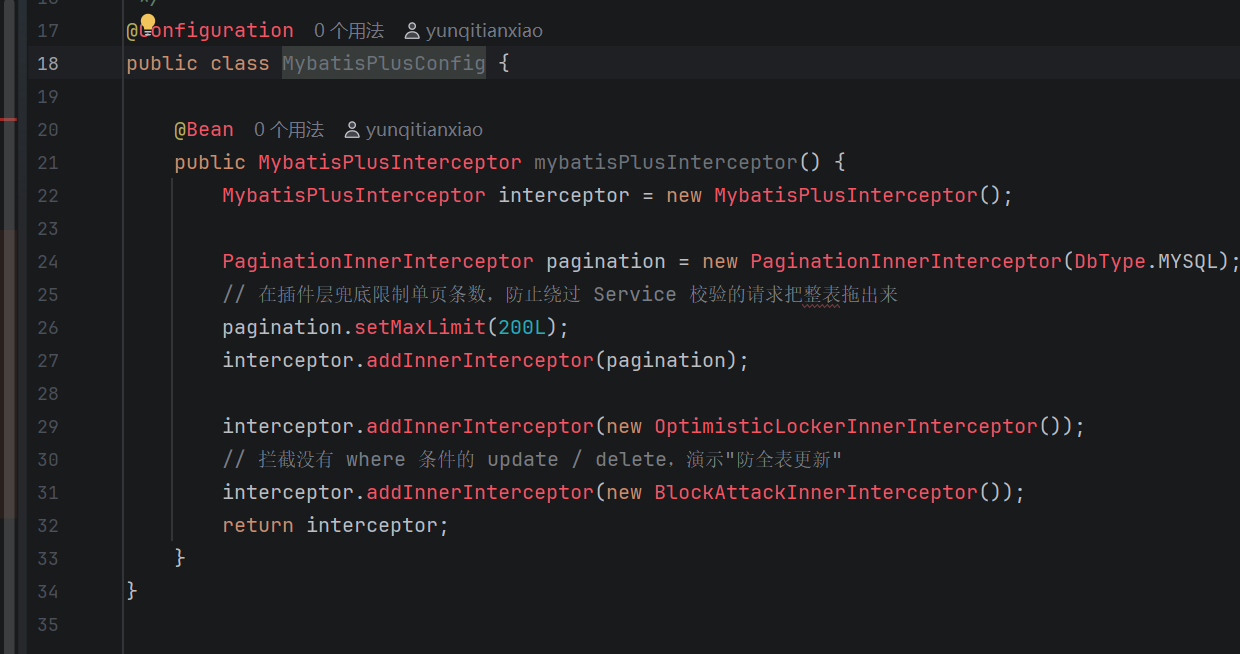
\includegraphics[width=\linewidth]{media/image44.png}

\subsubsection*{8.2.2 插件顺序是硬约束}\label{sec:mp-order}
\addcontentsline{toc}{subsubsection}{8.2.2 插件顺序是硬约束}

分页插件自动做 count 与分页，无需手写 limit。乐观锁用 OptimisticLockerInnerInterceptor 加 @Version，并发编辑返回 40900 而非静默覆盖。防全表更新用 BlockAttackInnerInterceptor，没有 where 的 update 和 delete 会被拦截。

三者构成有序拦截链，顺序错了会出现分页失效或乐观锁不生效，却没有任何报错，属于静默失败。这里按官方建议排列，依次是分页、乐观锁、防全表。

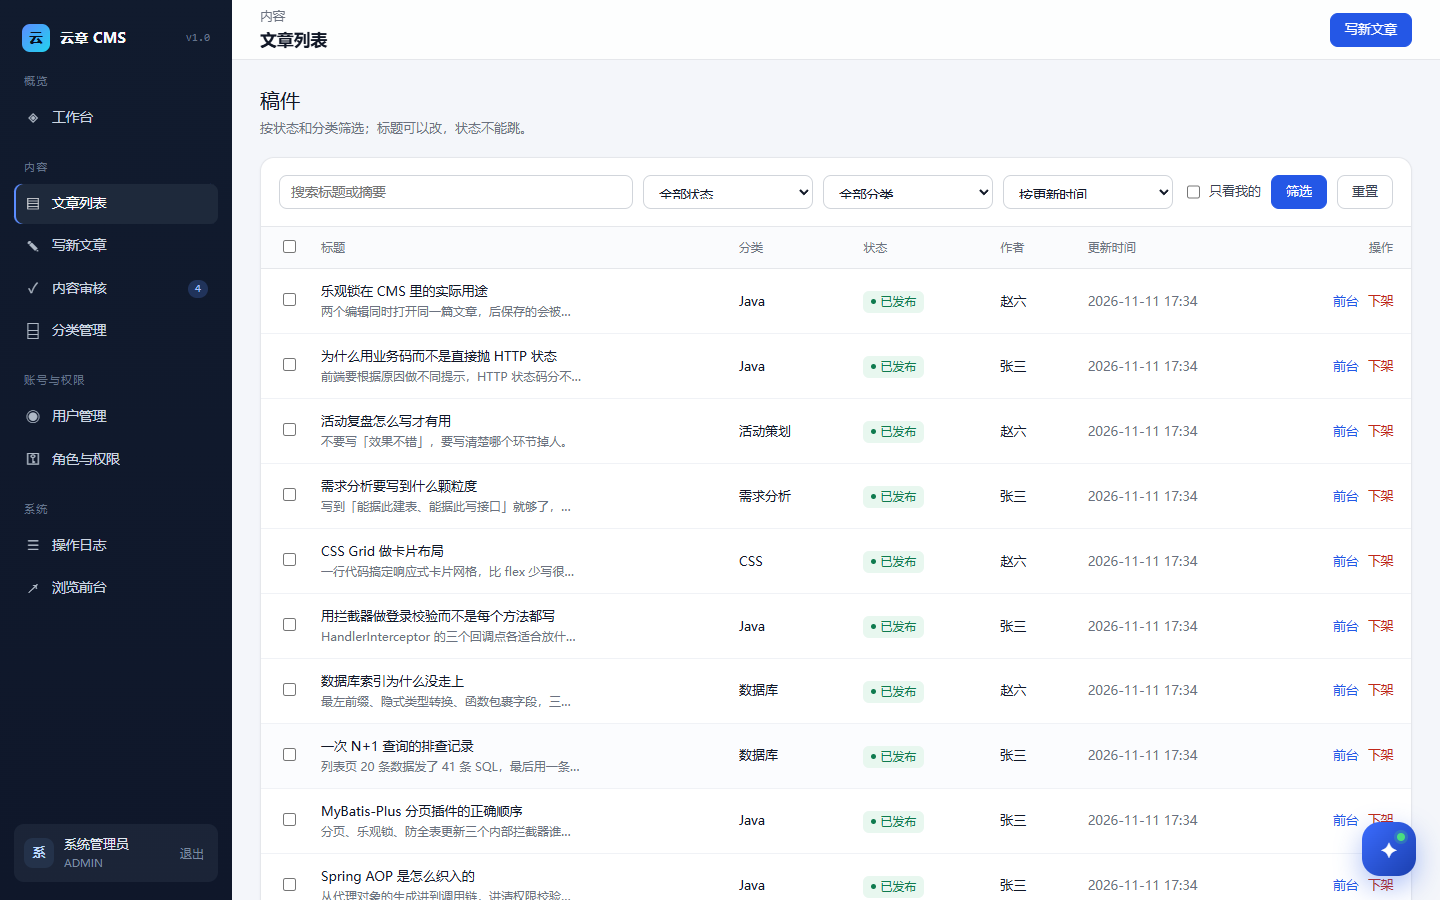
\includegraphics[width=\linewidth]{media/image45.png}

\subsubsection*{8.2.3 条件构造器}\label{sec:mp-wrapper}
\addcontentsline{toc}{subsubsection}{8.2.3 条件构造器}

条件构造器用 LambdaQueryWrapper，字段引用类型安全，避免手写列名。逻辑删除用 @TableLogic 全局开关，所有查询自动过滤；自动填充用 MetaObjectHandler，审计四字段统一写入，这两点见 8.1。

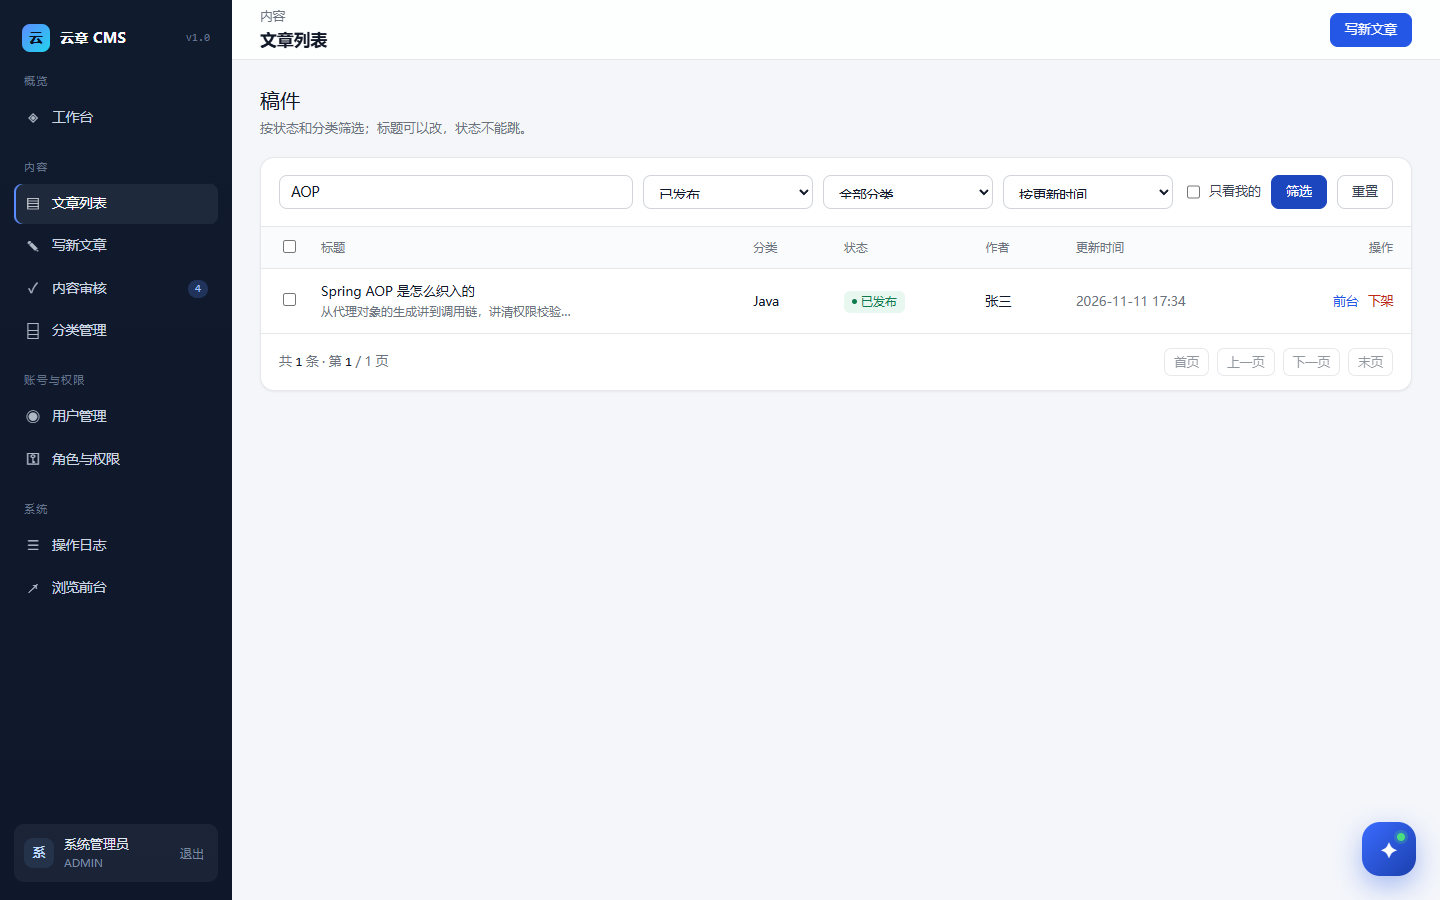
\includegraphics[width=\linewidth]{media/image46.png}

\subsection*{8.3 SQL 专项优化：列表页的 N+1}\label{sql-ux4e13ux9879ux4f18ux5316ux5217ux8868ux9875ux7684-n1}
\addcontentsline{toc}{subsection}{8.3 SQL 专项优化：列表页的 N+1}

这一章只解决一个问题：列表页从 1+N 条 SQL 降到 2 条。

\subsubsection*{8.3.1 问题诊断}\label{sec:n1-diag}
\addcontentsline{toc}{subsubsection}{8.3.1 问题诊断}

朴素写法：1 条 SQL 查 20 条文章，循环里再各查 20 次分类名和作者名，共 41 条 SQL。文章一多，查询次数线性上涨，列表页越来越慢。

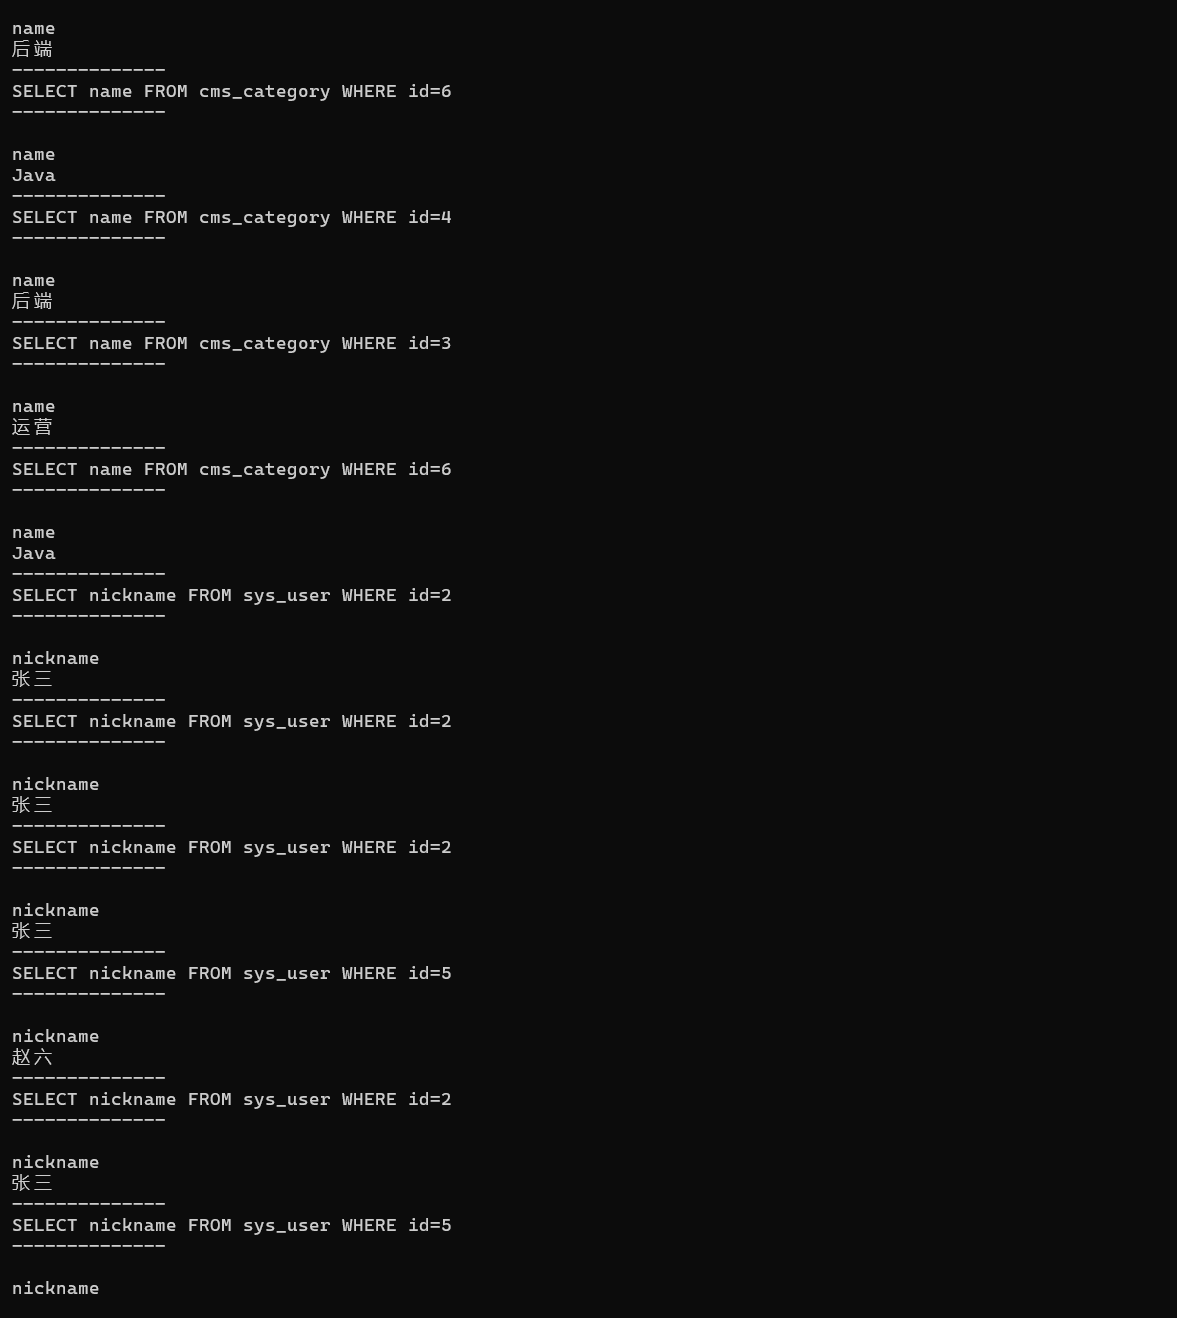
\includegraphics[width=\linewidth]{media/image47.png}

\subsubsection*{8.3.2 三表 join 方案}\label{sec:n1-join}
\addcontentsline{toc}{subsubsection}{8.3.2 三表 join 方案}

一条三表 join 把展示所需字段一次带出：

\begin{verbatim}
<sql id="baseFrom">
FROM cms_article a
LEFT JOIN cms_category c ON c.id = a.category_id
LEFT JOIN sys_user u1 ON u1.id = a.author_id
LEFT JOIN sys_user u2 ON u2.id = a.auditor_id
WHERE a.deleted = 0
</sql>
\end{verbatim}

配合分页插件，列表页总共 \textbf{2 条 SQL}（count + 数据）。

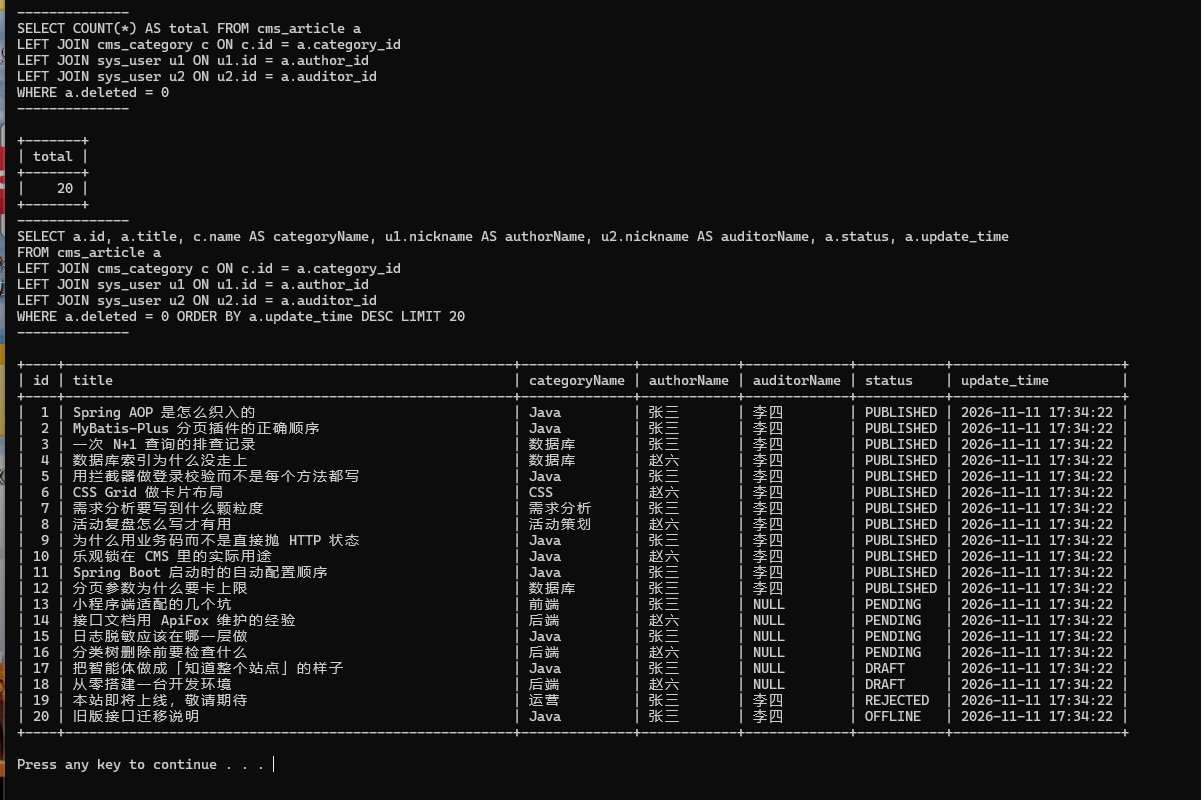
\includegraphics[width=\linewidth]{media/image48.png}

\subsubsection*{8.3.3 判据与索引配合}\label{sec:n1-criteria}
\addcontentsline{toc}{subsubsection}{8.3.3 判据与索引配合}

判据不是"看起来变快了"，而是把 mapper 日志开到 DEBUG 数 SQL 条数。动态条件全部用 \#\{\} 预编译；只有 ORDER BY 使用 \$\{\}，而它的值只可能由 SortWhitelist 从白名单生成。idx\_article\_query 覆盖默认视图的过滤与排序组合，分页插件限制单页 200 条。

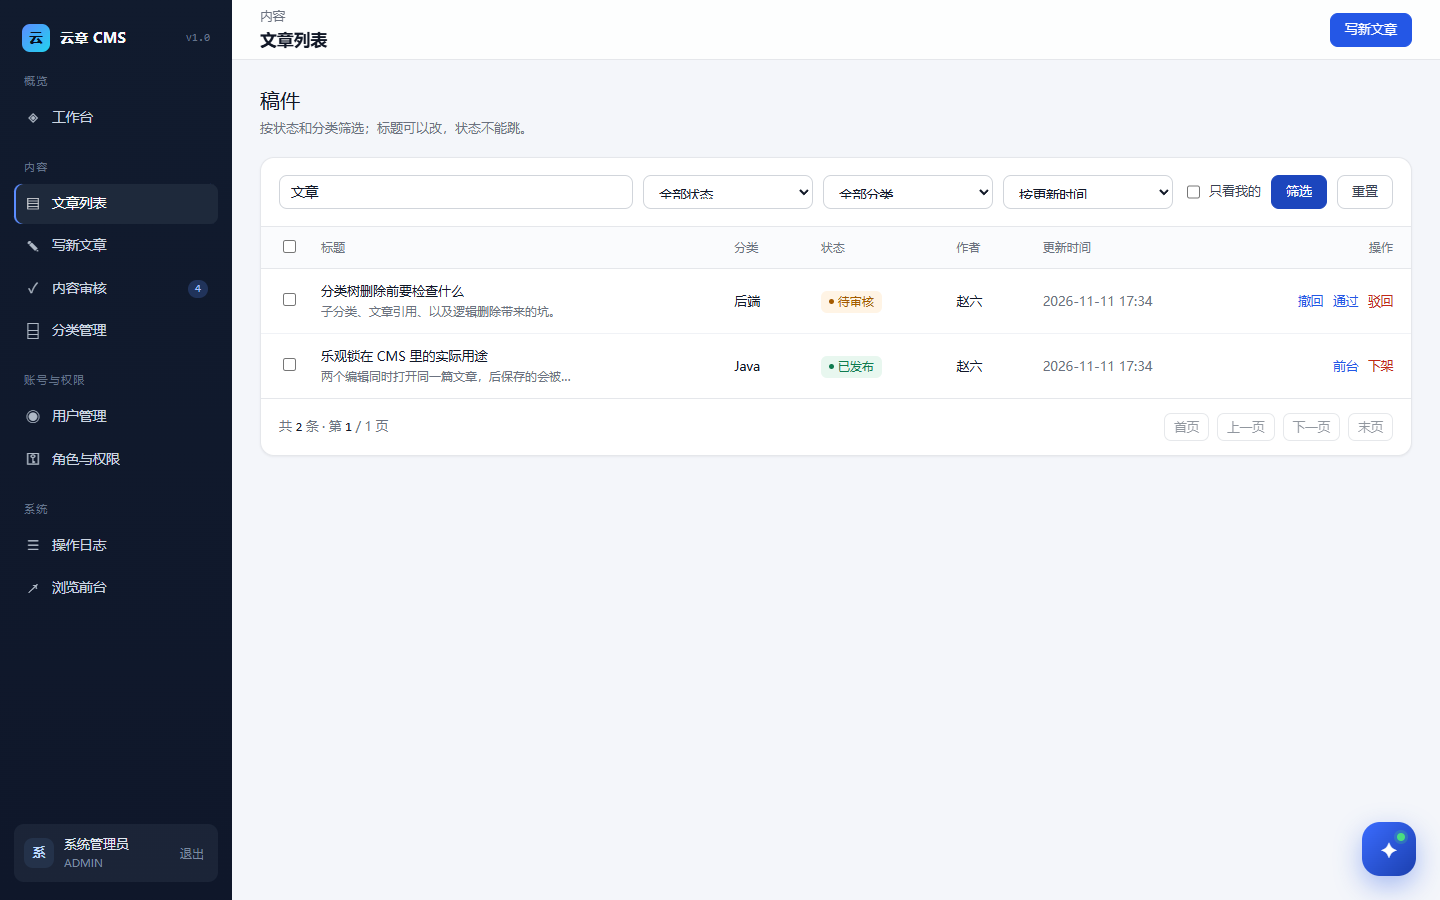
\includegraphics[width=\linewidth]{media/image49.png}

\subsection*{8.4 RESTful 接口与 ApiFox 联调}\label{restful-ux63a5ux53e3ux4e0e-apifox-ux8054ux8c03}
\addcontentsline{toc}{subsection}{8.4 RESTful 接口与 ApiFox 联调}

这一章说明统一返回结构、五位业务码，以及 OpenAPI 与 ApiFox 的对账。

\subsubsection*{8.4.1 统一返回结构}\label{sec:rest-result}
\addcontentsline{toc}{subsubsection}{8.4.1 统一返回结构}

统一返回结构如下：

\begin{verbatim}
{
  "code": 0,
  "message": "成功",
  "data": {},
  "traceId": "8f3c1a2e"
}
\end{verbatim}

HTTP 状态码表达协议层结果，业务码表达具体原因，二者分开。

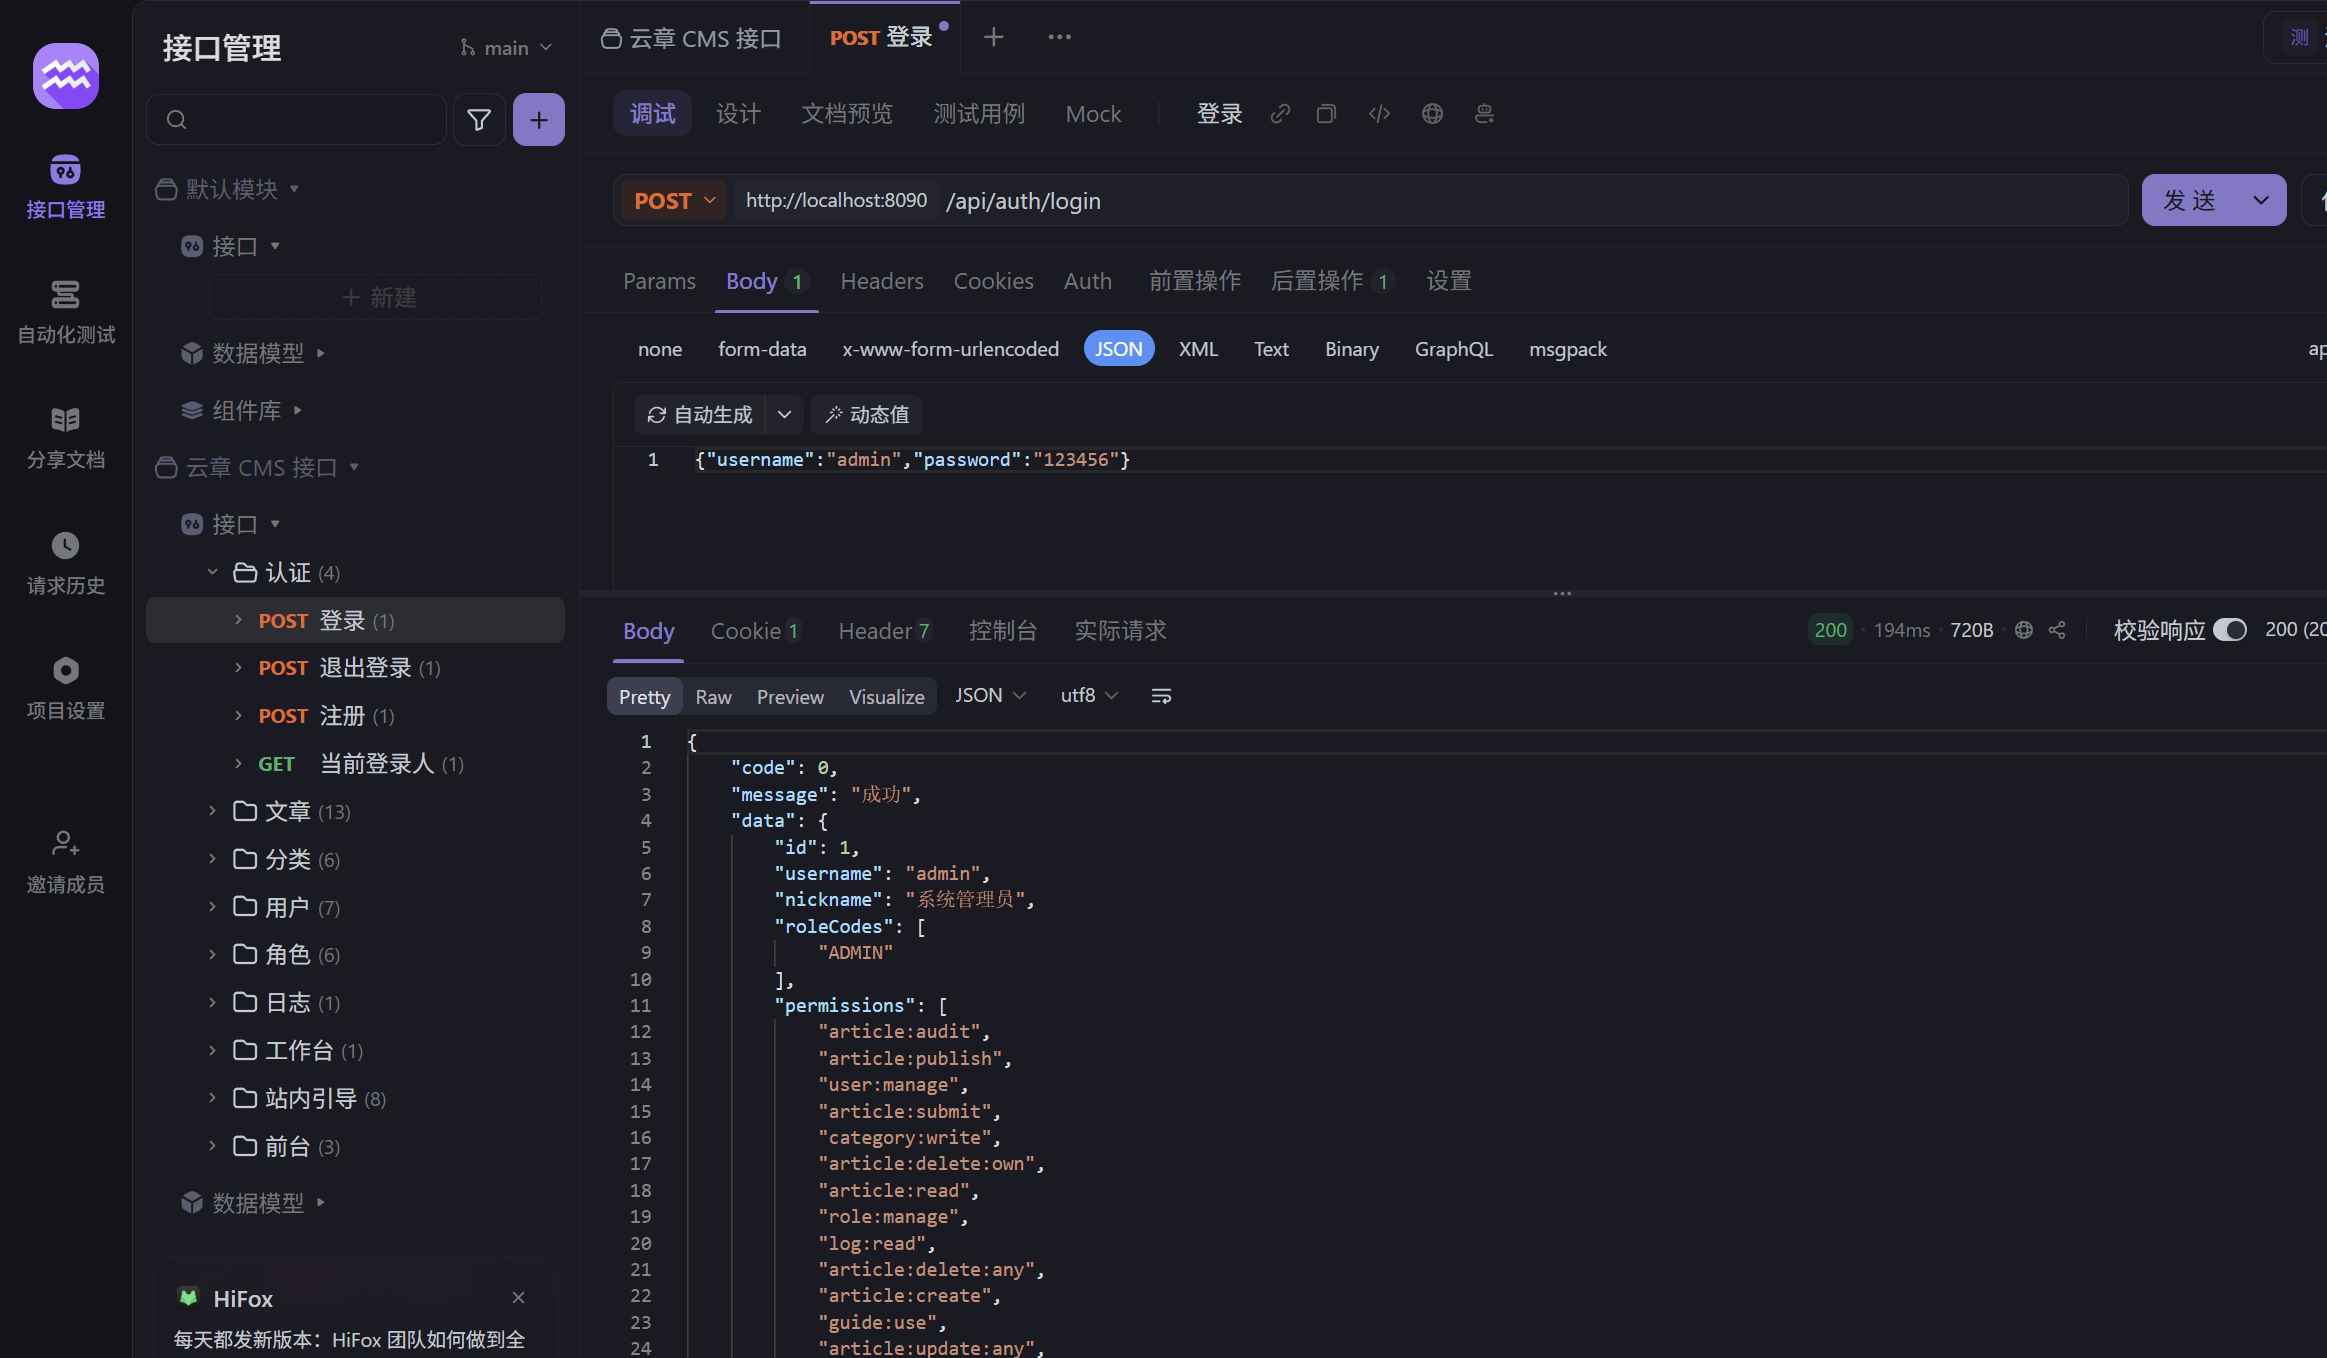
\includegraphics[width=\linewidth]{media/image50.png}

\subsubsection*{8.4.2 业务码设计}\label{sec:rest-code}
\addcontentsline{toc}{subsubsection}{8.4.2 业务码设计}

\begin{longtable}{@{}>{\raggedright\arraybackslash}p{3.2cm}>{\raggedright\arraybackslash}p{7.2cm}>{\raggedright\arraybackslash}p{1.8cm}@{}}
\toprule
\textbf{业务码} & \textbf{含义} & \textbf{HTTP} \\
\midrule
\endfirsthead
\multicolumn{3}{@{}l}{\small（续表）}\\
\toprule
\textbf{业务码} & \textbf{含义} & \textbf{HTTP} \\
\midrule
\endhead
0 & 成功 & 200 \\
40000 & 参数不合法 & 400 \\
40001 & 分类层级超限 & 400 \\
40003 & 内容含敏感信息 & 400 \\
40100 / 40101 / 40102 & 未登录 / 密码错 / 账号停用 & 401 \\
40300 / 40301 & 无权限 / 非本人数据 & 403 \\
40400 & 资源不存在 & 404 \\
40900 / 40901 / 40902 / 40903 & 版本冲突 / 状态不允许 / 重复 / 被引用 & 409 \\
50000 / 50001 & 系统错误 / 数据库错误 & 500 \\
\bottomrule
\end{longtable}

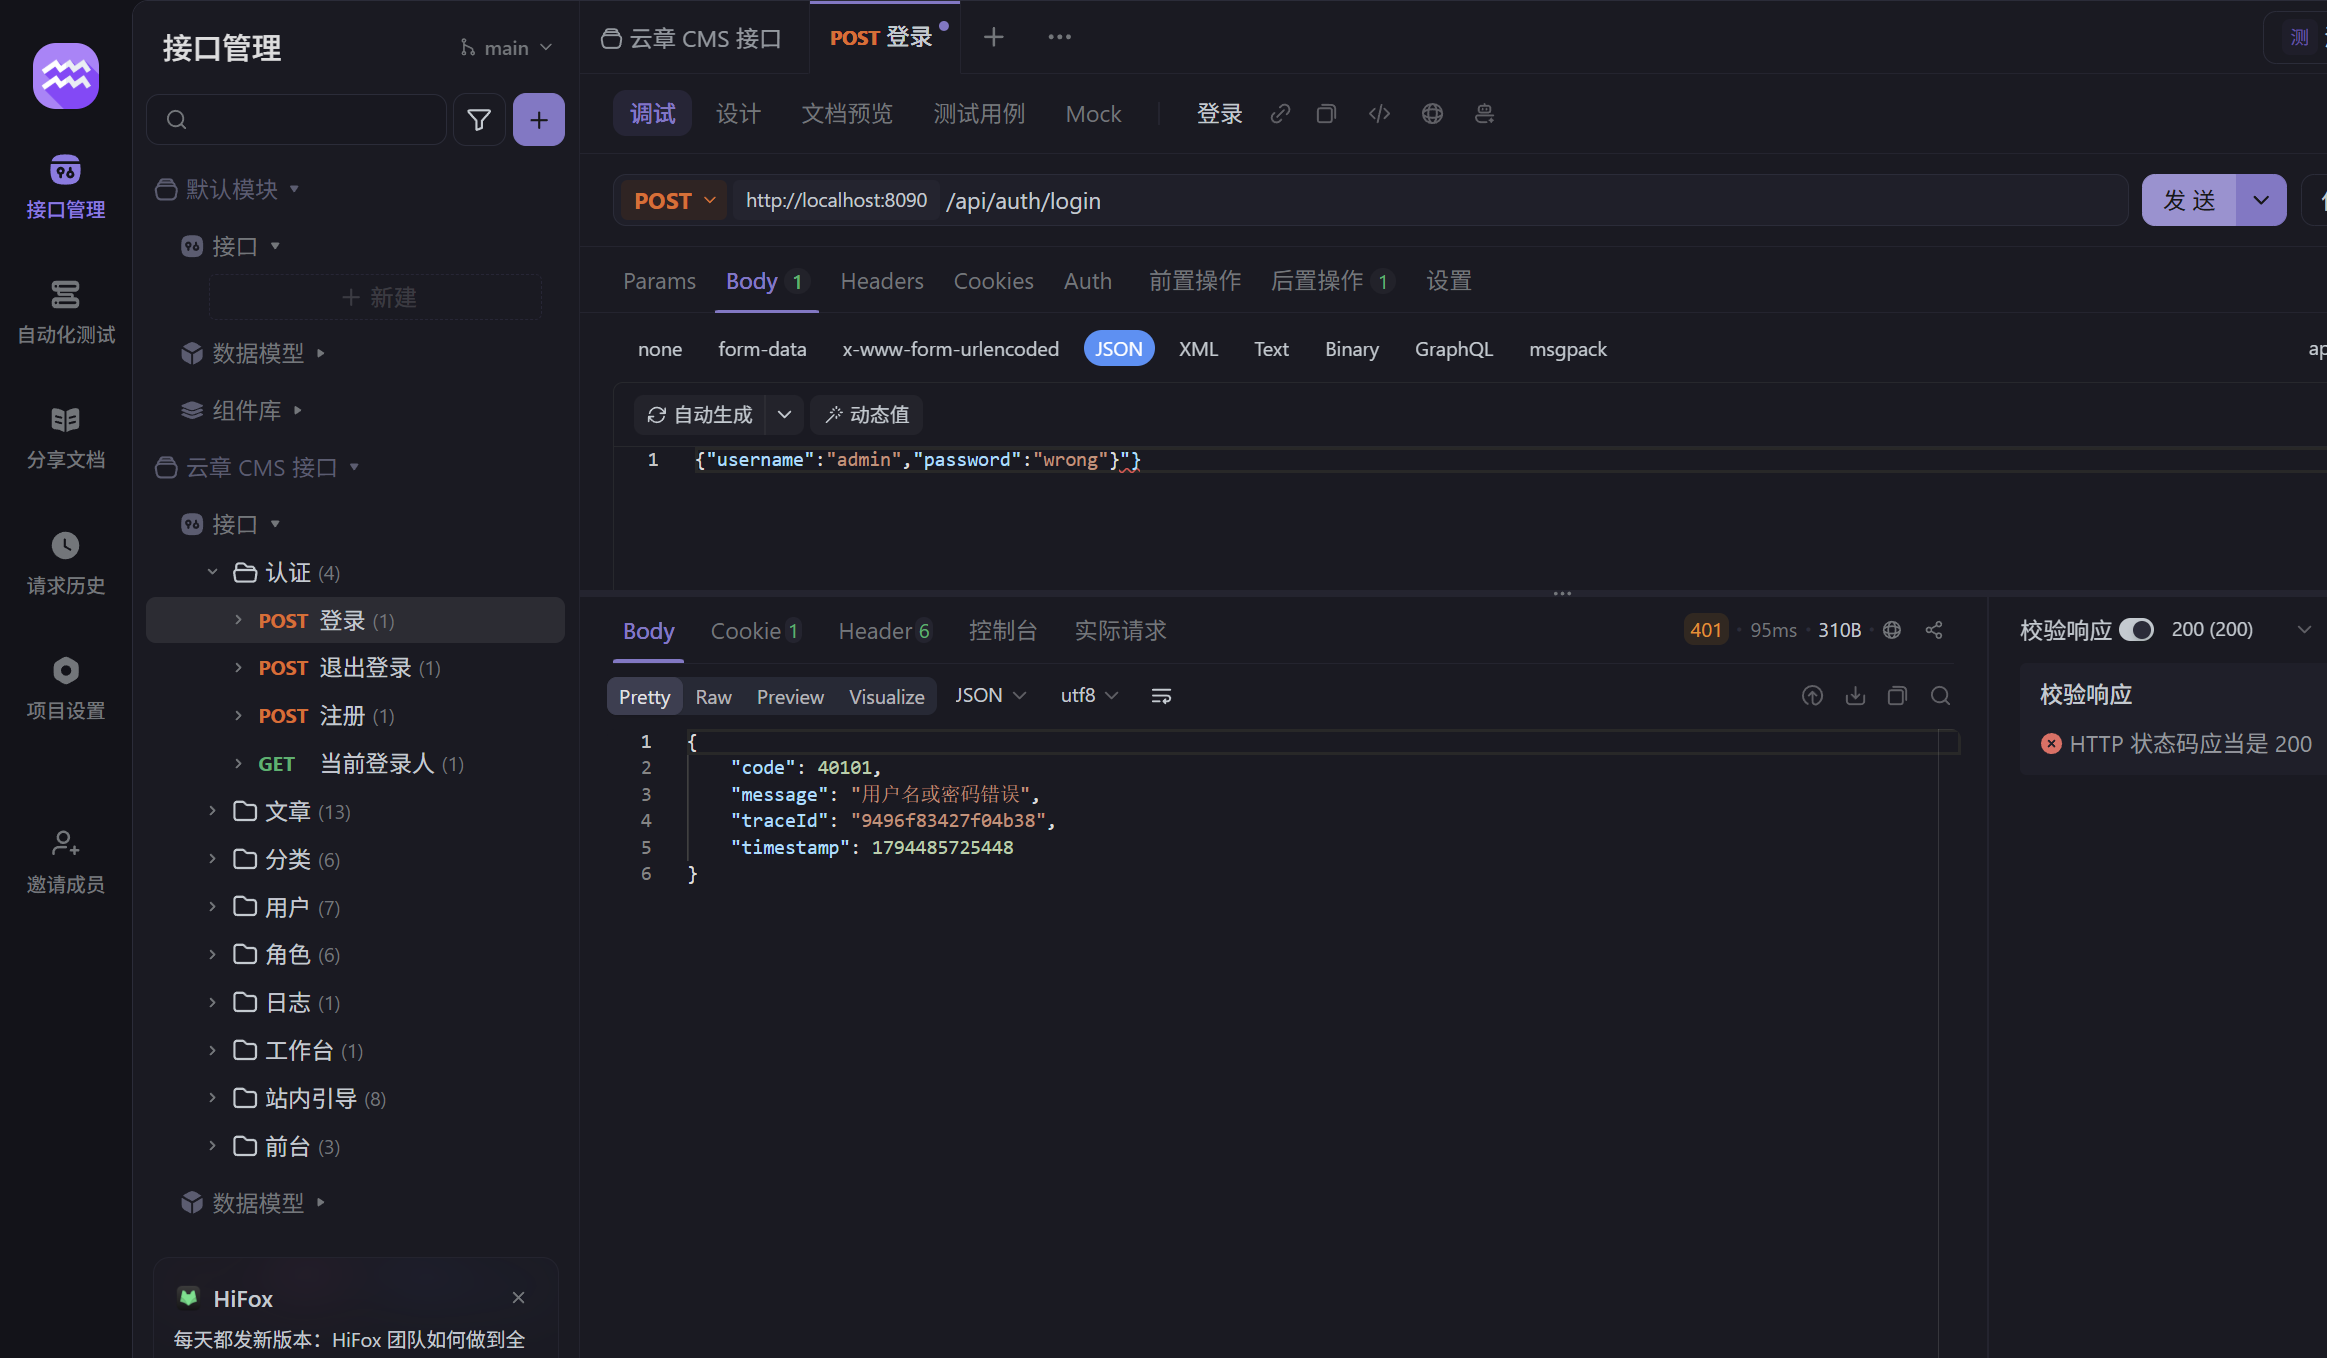
\includegraphics[width=\linewidth]{media/image51.png}

\subsubsection*{8.4.3 OpenAPI 与 ApiFox 联调}\label{sec:rest-apifox}
\addcontentsline{toc}{subsubsection}{8.4.3 OpenAPI 与 ApiFox 联调}

接口文档与联调上，apifox/cms-openapi.json 采用 OpenAPI 3.0，可直接导入 ApiFox。文档与实现用脚本对账，49 个操作、50 个 schema、37 条路径与 Controller 双向差集为空。也就是说，没有文档里有而代码里没有的接口，也没有相反的情况。

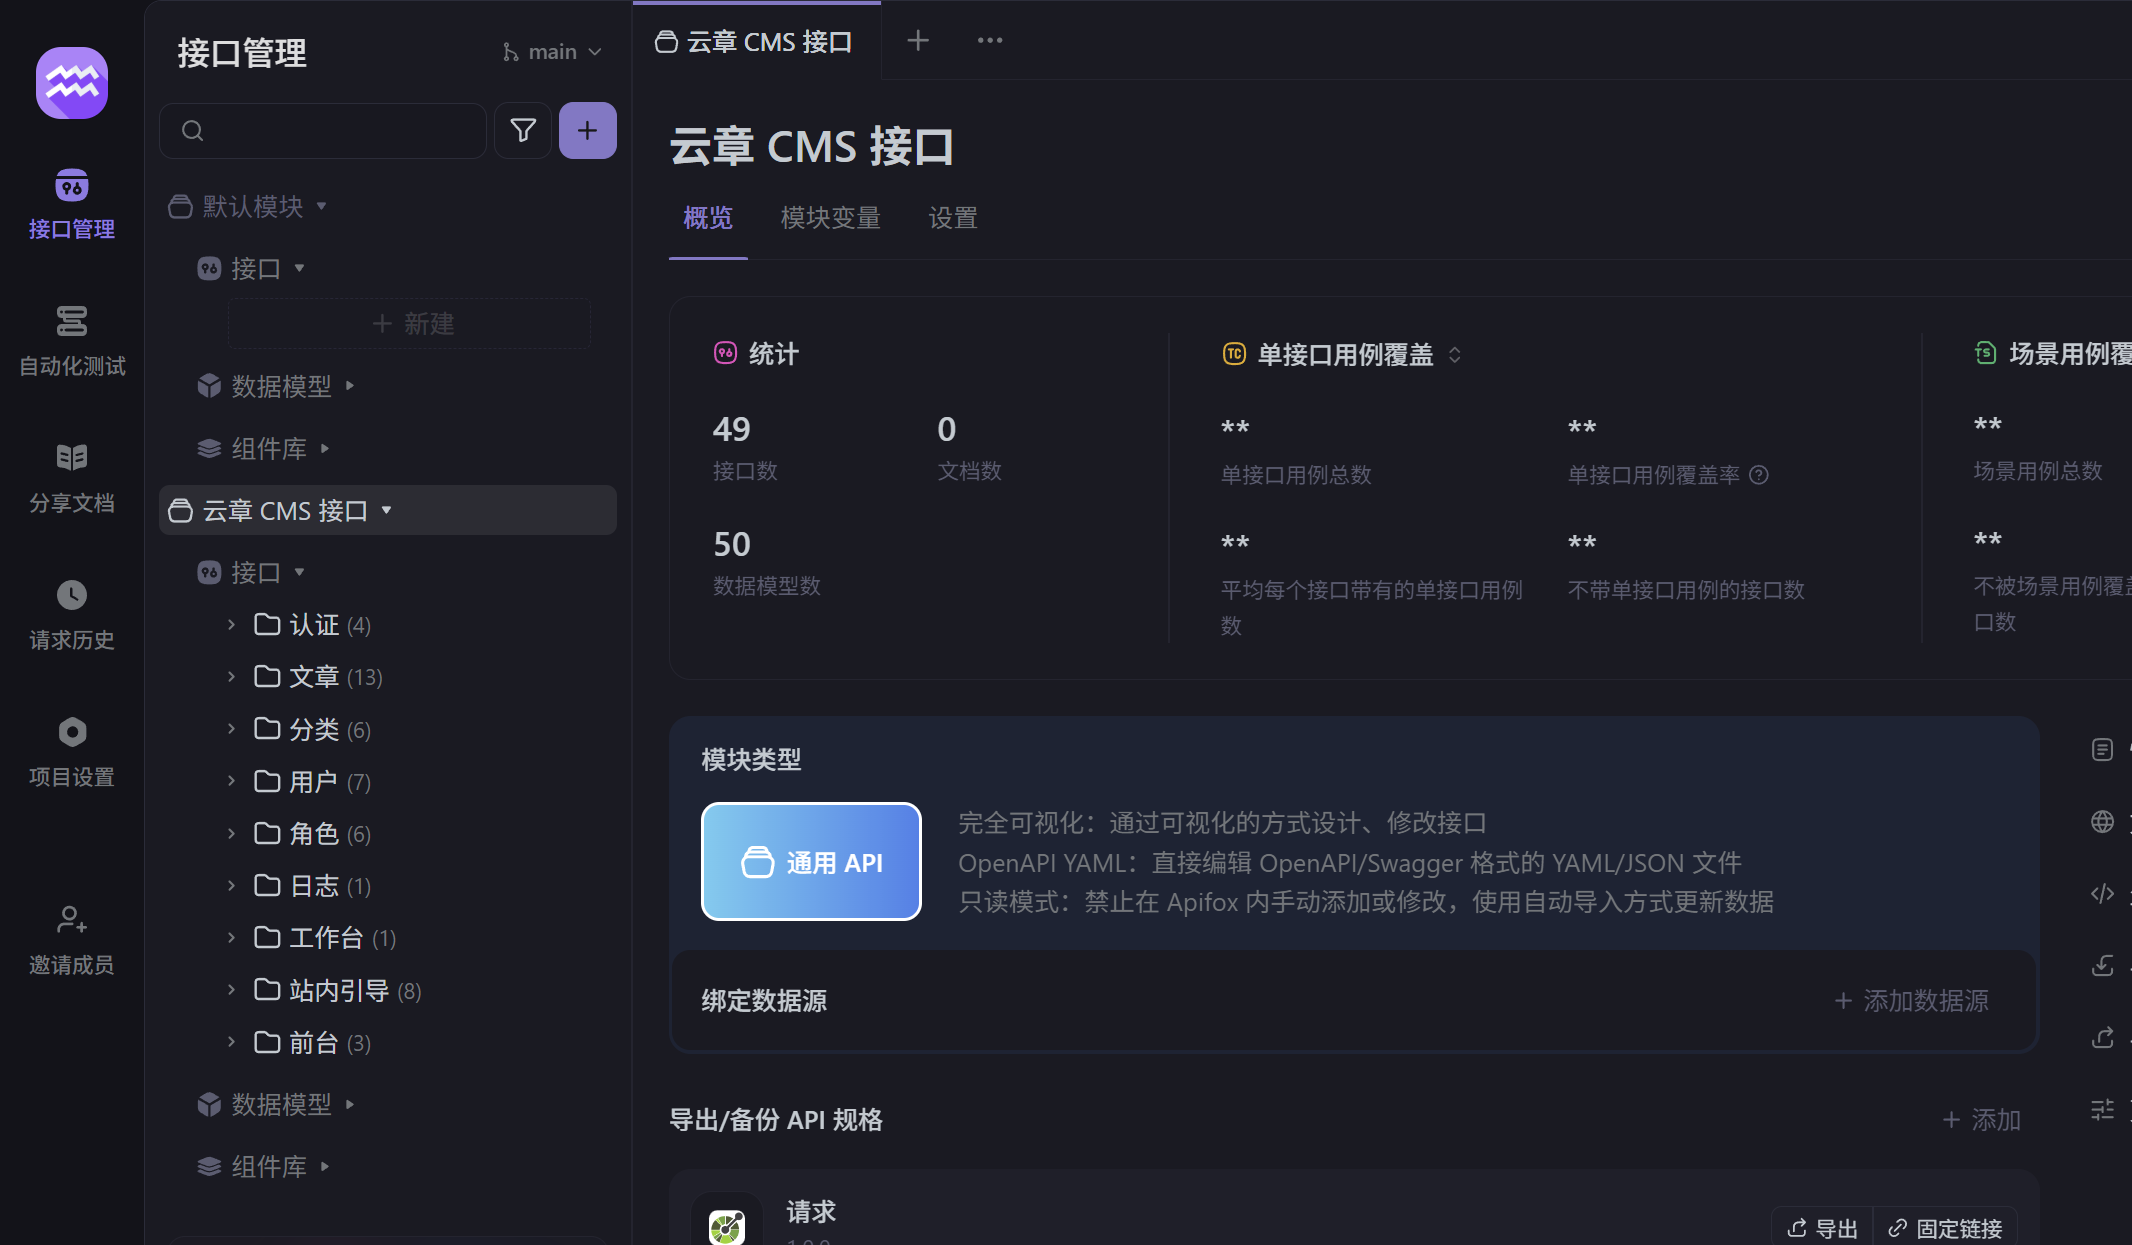
\includegraphics[width=\linewidth]{media/image52.png}

\subsection*{8.5 站内引导智能体（附加模块）}\label{ux7ad9ux5185ux5f15ux5bfcux667aux80fdux4f53ux9644ux52a0ux6a21ux5757}
\addcontentsline{toc}{subsection}{8.5 站内引导智能体（附加模块）}

这是一个差异化模块，但它的设计原则与主线一致，就是不假装能力。

本模块接口与功能说明如下表。

\begin{longtable}{@{}>{\raggedright\arraybackslash}p{8.4cm}>{\raggedright\arraybackslash}p{4.4cm}@{}}
\toprule
\textbf{接口名称} & \textbf{功能说明} \\
\midrule
\endfirsthead
\multicolumn{2}{@{}l}{\small（续表）}\\
\toprule
\textbf{接口名称} & \textbf{功能说明} \\
\midrule
\endhead
\multicolumn{2}{@{}l}{\textbf{站内引导} \quad /api/guide} \\
\midrule
GET /api/guide/pages & 查询全部页面卡片 \\
POST /api/guide/chat & 提问引导 \\
GET /api/guide/suggestions & 查询快捷问题 \\
GET /api/guide/llm & 查询模型通道状态 \\
PUT /api/guide/llm & 配置模型密钥 \\
DELETE /api/guide/llm & 清除模型密钥 \\
POST /api/guide/llm/test & 测试模型连通性 \\
GET /api/guide/selfcheck & 站点地图自检 \\
\bottomrule
\end{longtable}

引导问答处理流程如下（时序详见 5.4）。

\begin{center}
\begin{tikzpicture}[
  node distance=5mm,
  box/.style={rectangle, draw, rounded corners=1pt, align=center, minimum width=5.6cm, minimum height=0.72cm, font=\small},
  arr/.style={-{Stealth}}
]
\node[box] (a) {POST /api/guide/chat 收到提问};
\node[box, below=of a] (b) {IntentRouter 规则层中文 bigram 打分};
\node[box, below=of b] (c) {未命中且模型可用时，发给模型候选卡片摘要};
\node[box, below=of c] (d) {校验返回卡片 id 在站点地图内};
\node[box, below=of d] (e) {返回卡片，前端渲染};
\draw[arr] (a) -- (b);
\draw[arr] (b) -- (c);
\draw[arr] (c) -- (d);
\draw[arr] (d) -- (e);
\end{tikzpicture}
\end{center}



知道全站不是靠维护文档，而是靠启动期反射代码。SiteMapCollector 扫描 RequestMappingHandlerMapping，读取 @GuideCard 与 @RequirePermission。SiteMapValidator 执行 C1--C5 校验，包括卡片 id 唯一、受控 Controller 必须有卡片、权限码必须存在于 sys\_permission、yaml 不许凭空造页面、路由唯一非空。任何一条不通过，服务拒绝启动，某页面不在引导里就不会是演示时才发现的问题。

规则优先，模型兜底。规则层用中文 bigram 打分，命中直接返回，离线可用，未命中的短问句才走模型通道。

模型不产生内容。发给模型的是候选卡片的 id、title、summary，模型只回卡片 id，且必须是站点地图的子集，越界整体丢弃。卡片文案从不经过模型。

用户可自填模型密钥。PUT /api/guide/llm 只把密钥存入当前 HttpSession，任何接口只回显尾号。DELETE 回落服务端配置。POST /api/guide/llm/test 真发一次请求验证连通性。

\subsection*{8.6 界面实拍}\label{ux754cux9762ux5b9eux62cd}
\addcontentsline{toc}{subsection}{8.6 界面实拍}

登录页与工作台：

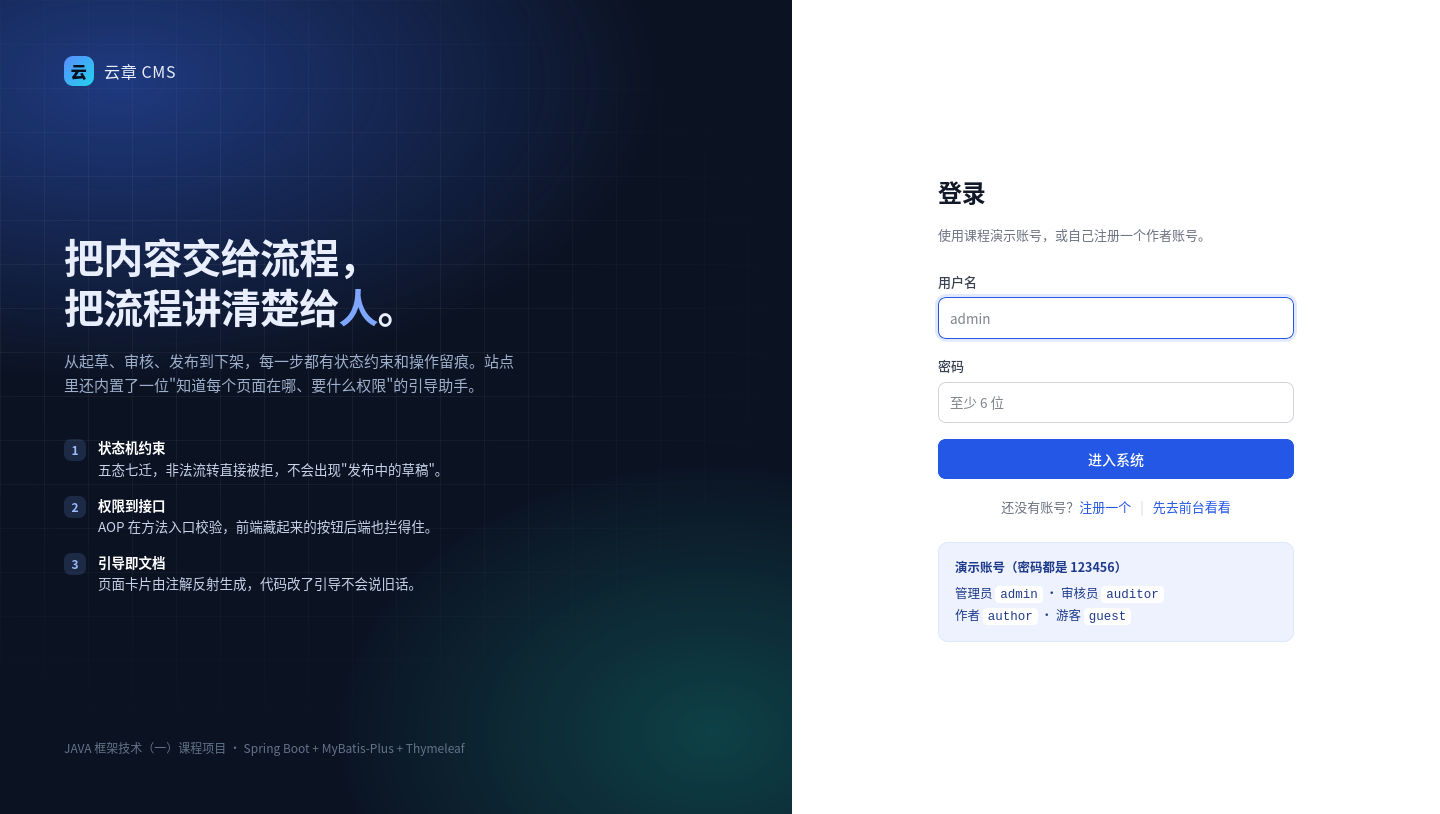
\includegraphics[width=\linewidth]{media/image6.png}

登录页

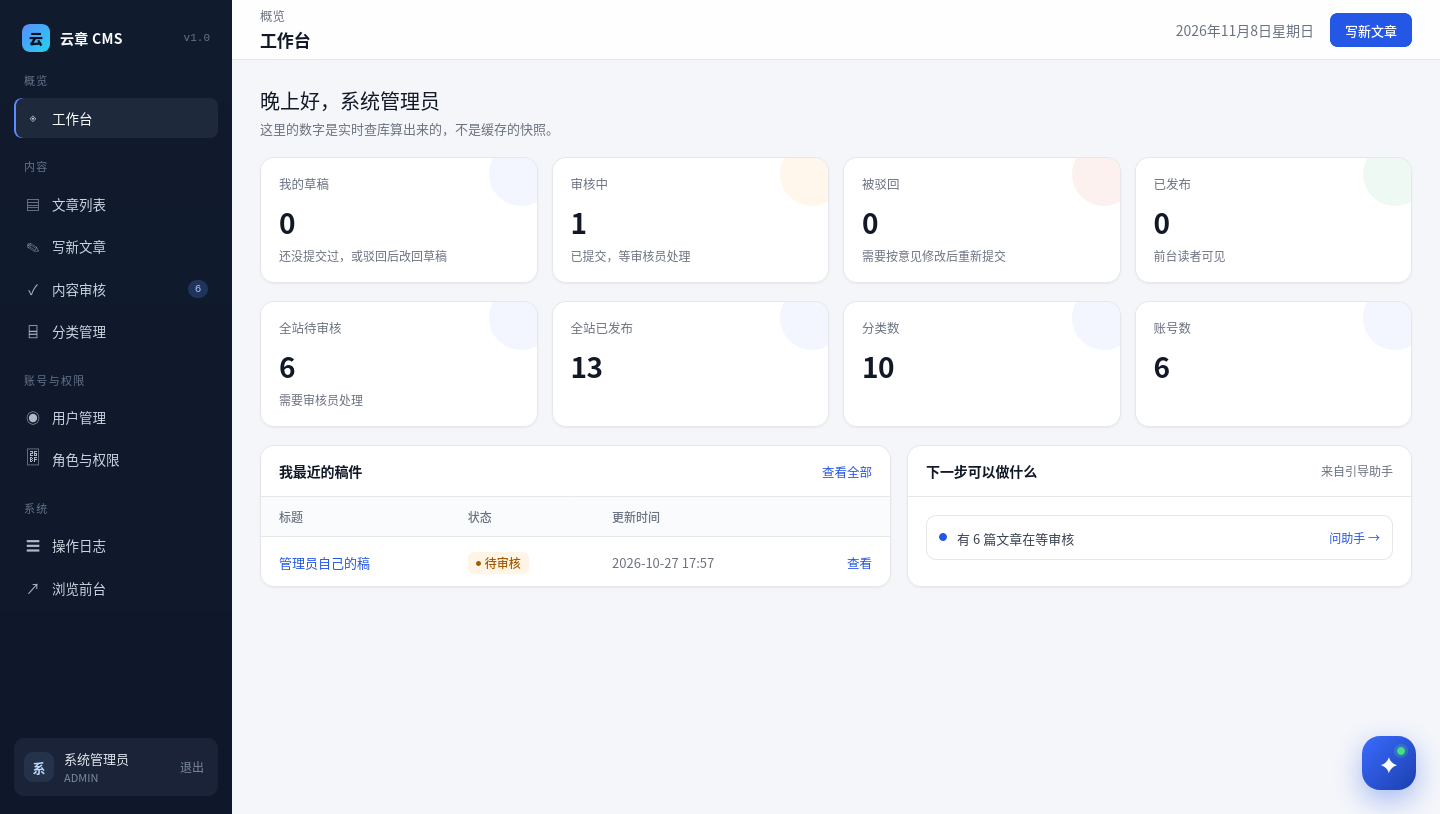
\includegraphics[width=\linewidth]{media/image7.png}

工作台：四张状态卡片与全站统计

文章列表（多条件筛选 + 批量操作）与写文章页：

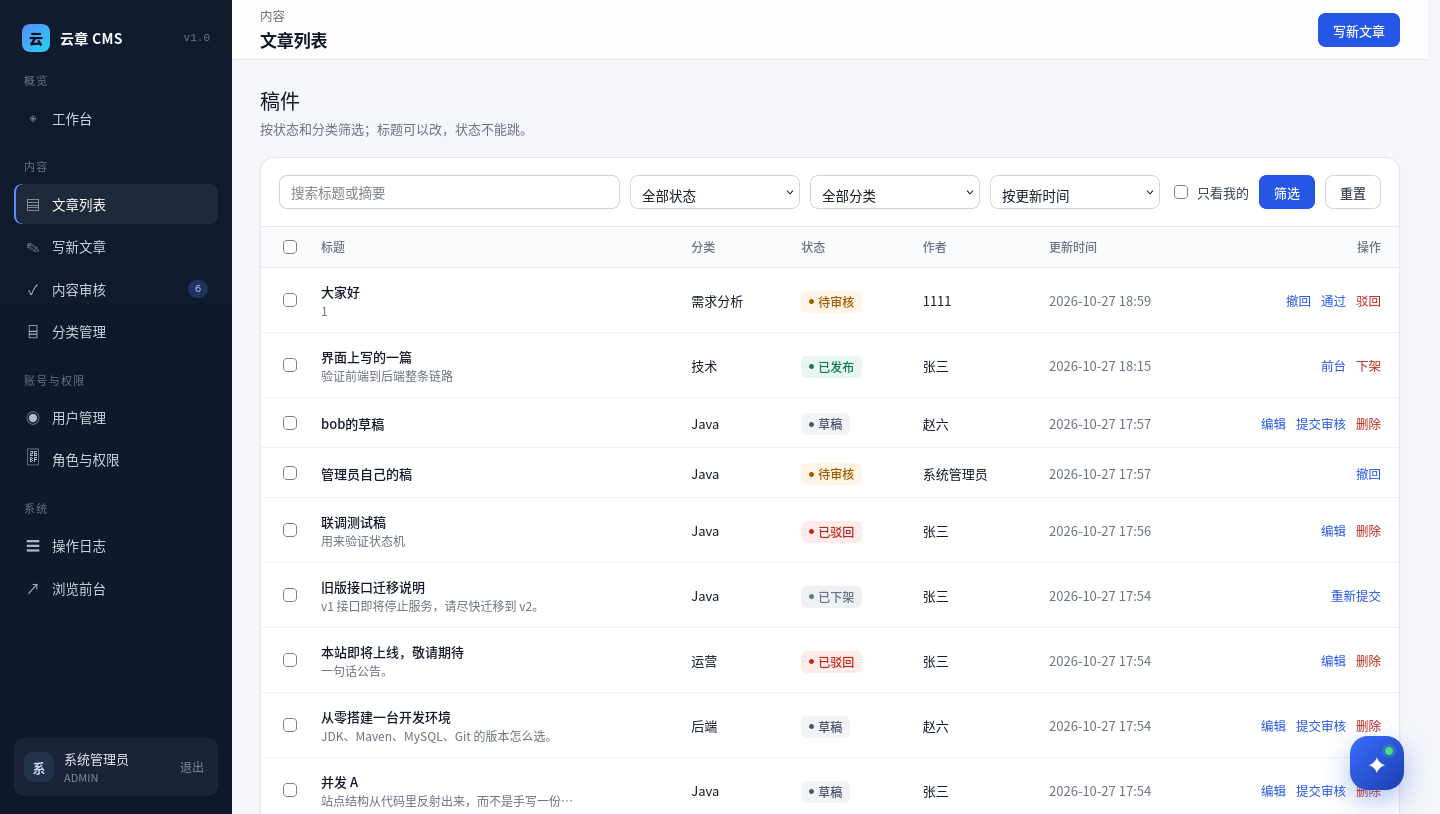
\includegraphics[width=\linewidth]{media/image8.png}

文章列表

内容审核与分类管理：

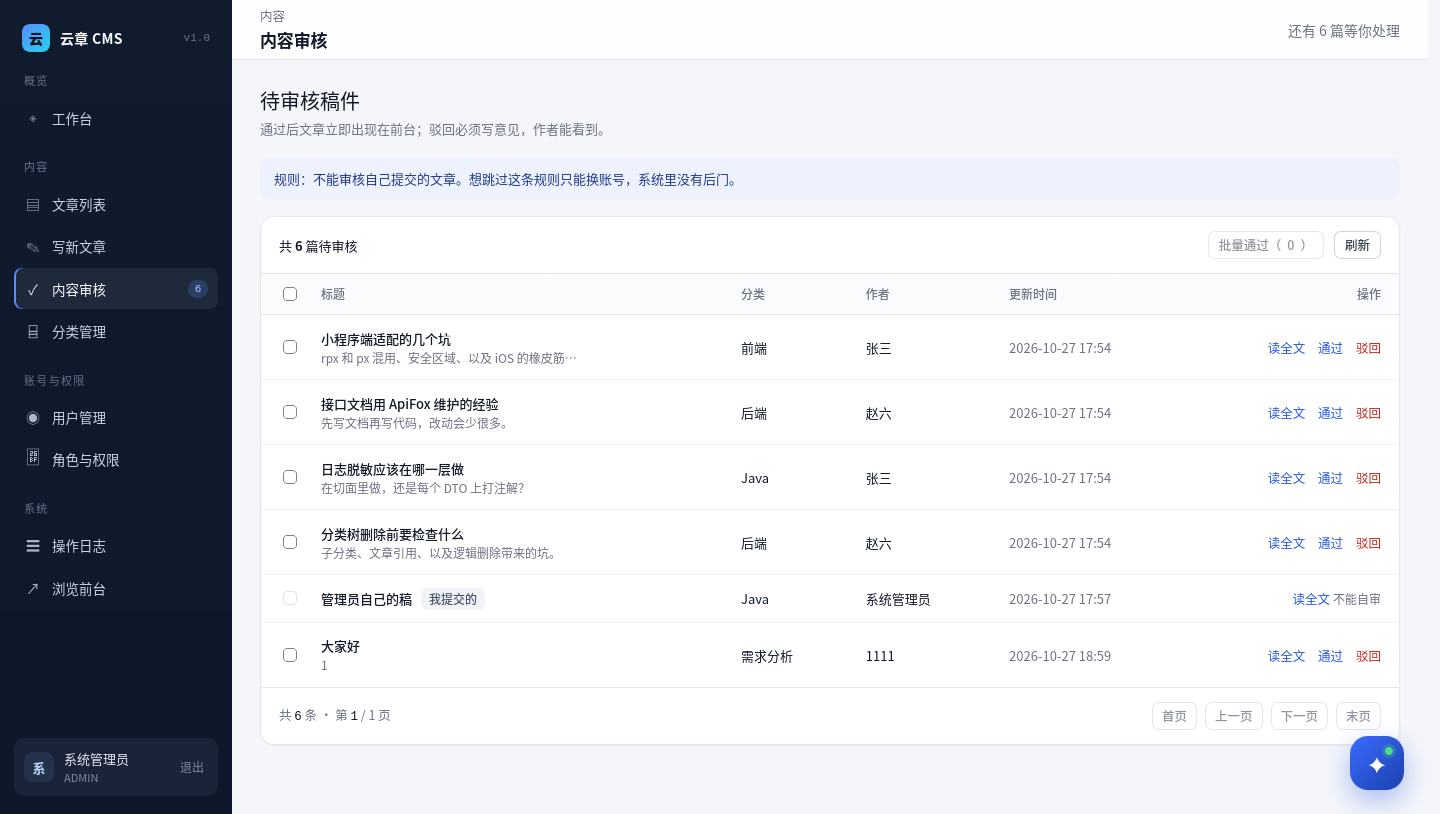
\includegraphics[width=\linewidth]{media/image9.png}

内容审核

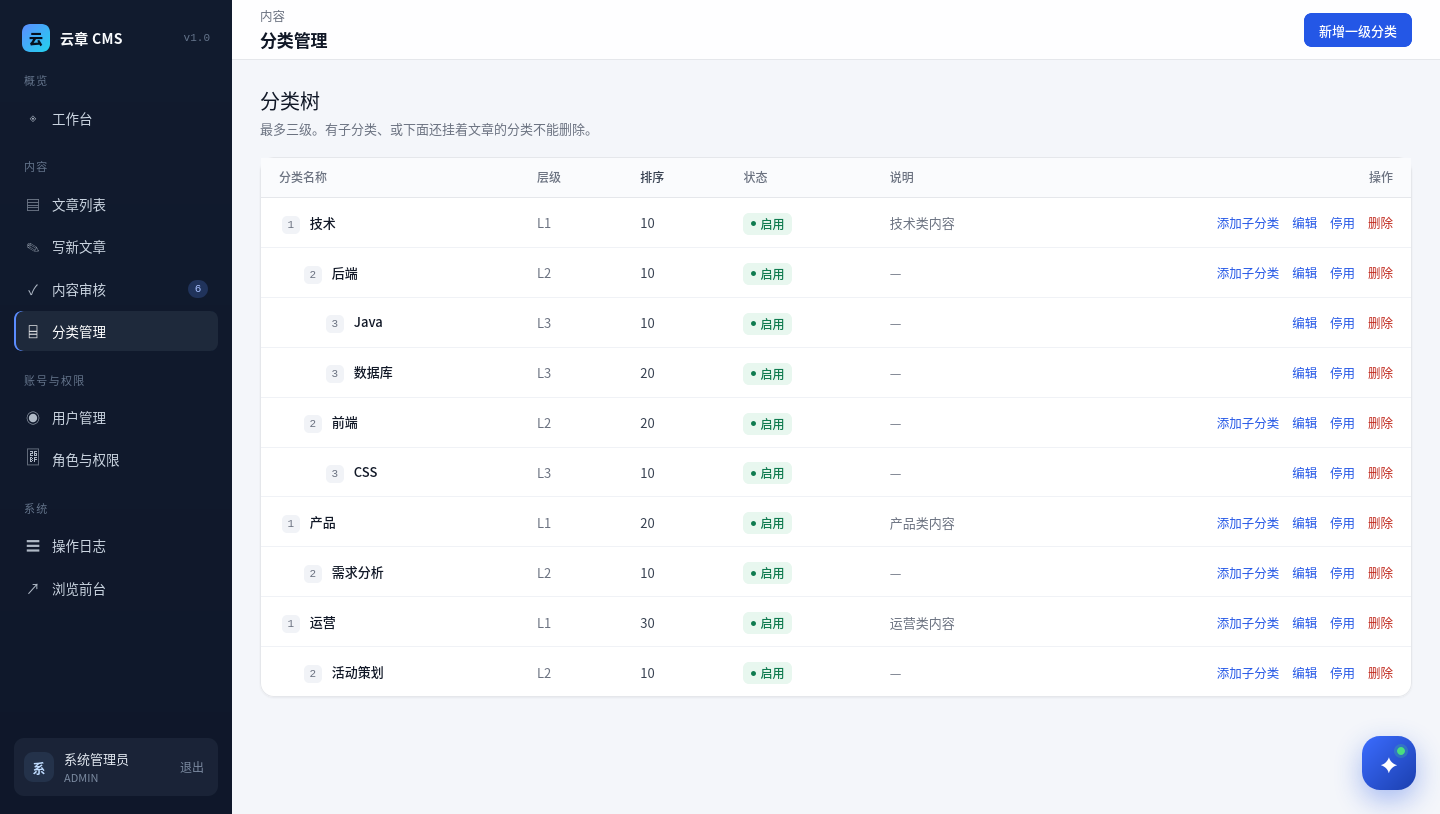
\includegraphics[width=\linewidth]{media/image10.png}

分类管理：三级树

用户与角色权限：

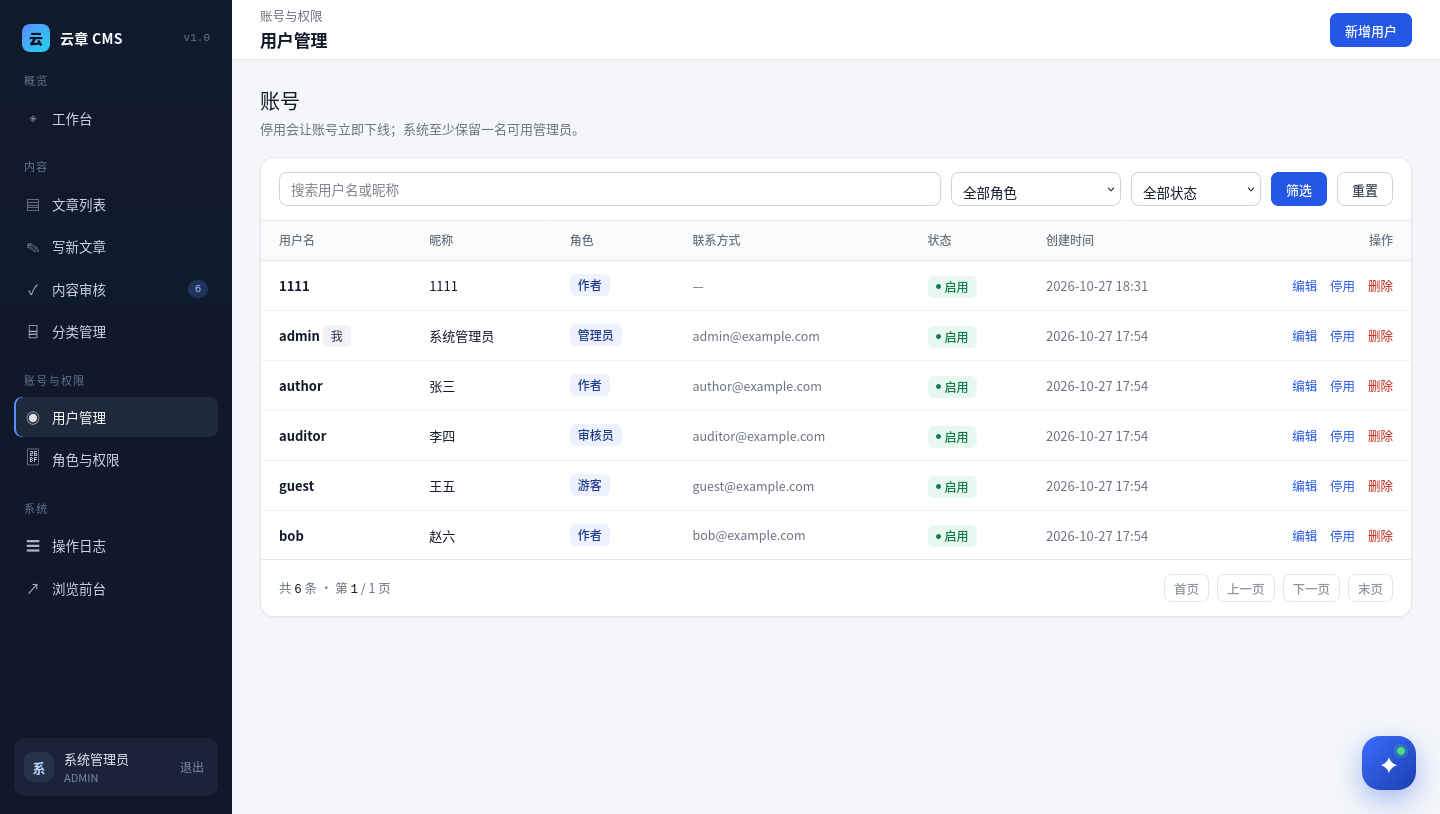
\includegraphics[width=\linewidth]{media/image11.png}

用户管理

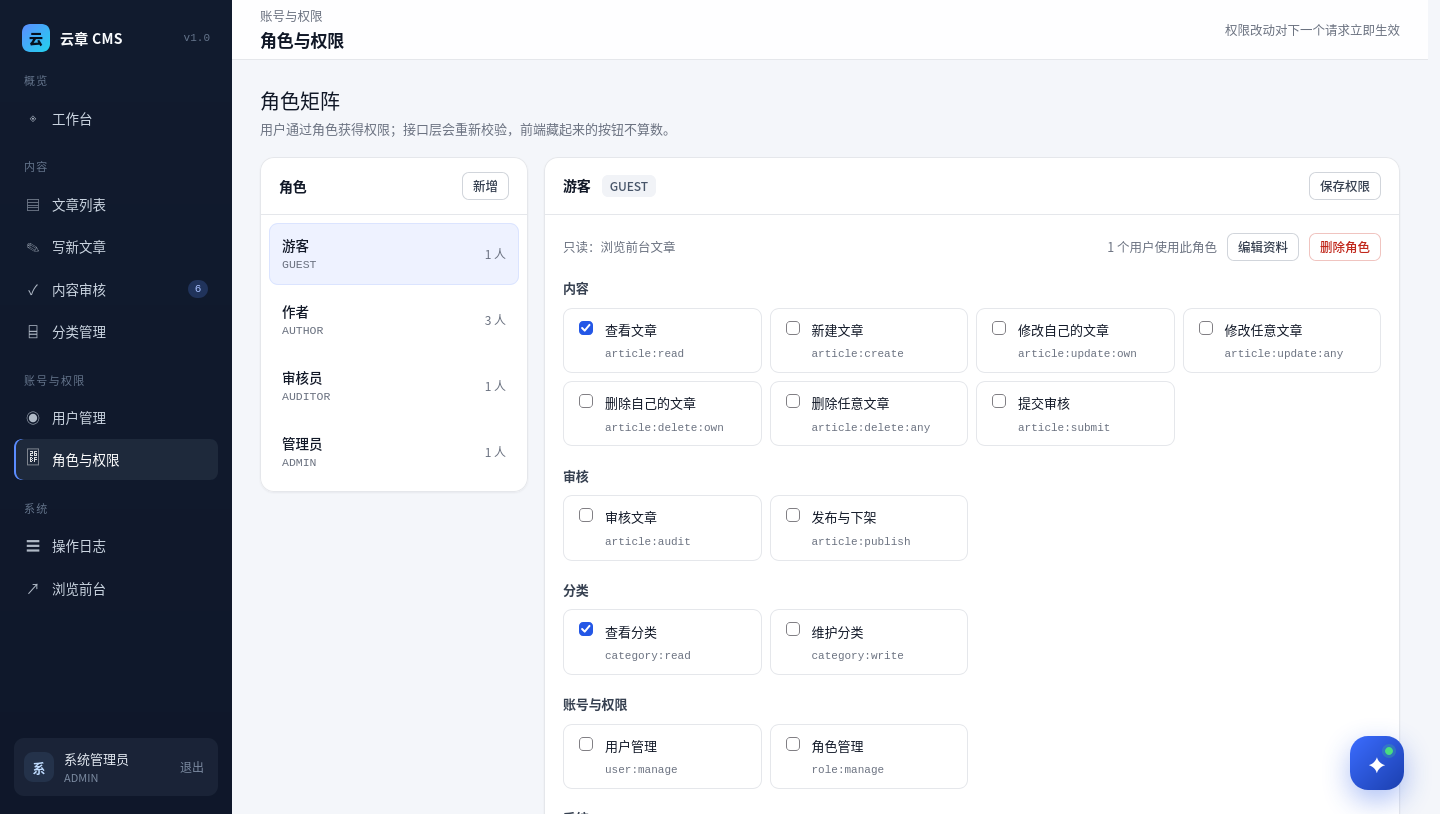
\includegraphics[width=\linewidth]{media/image12.png}

角色与权限

操作日志（含 DENIED 行）与前台阅读站：

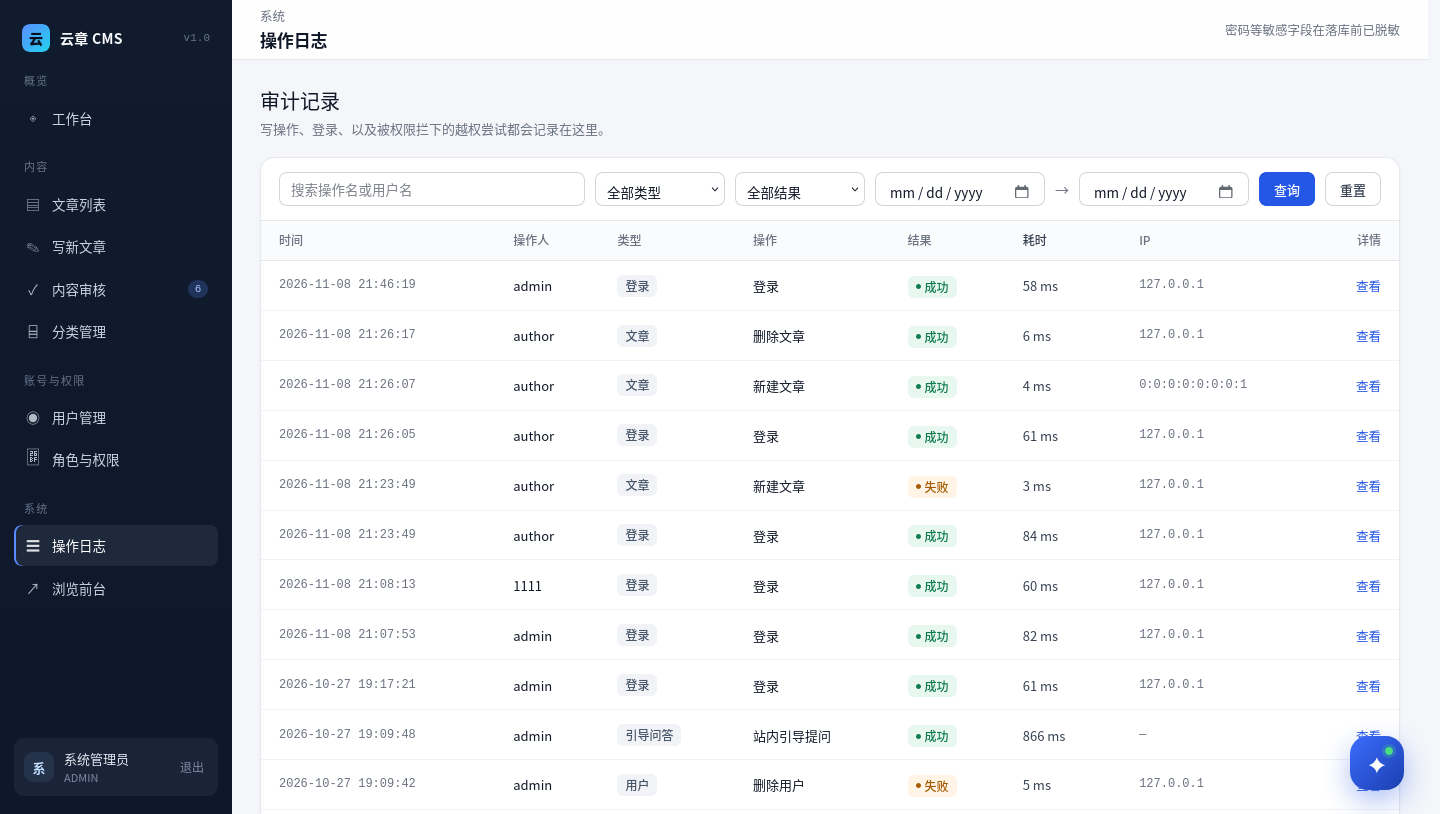
\includegraphics[width=\linewidth]{media/image13.png}

操作日志

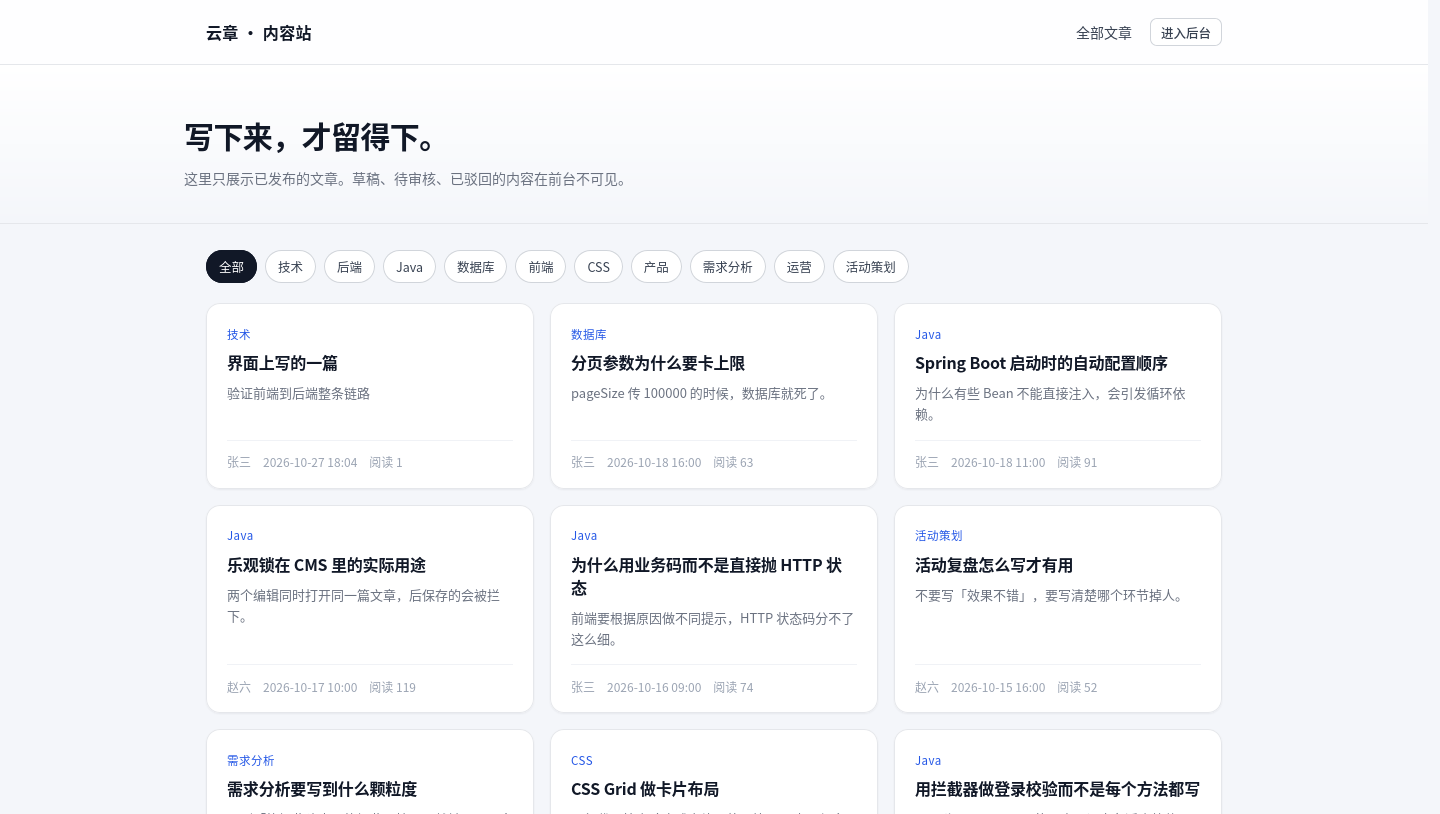
\includegraphics[width=\linewidth]{media/image14.png}

前台阅读站

站内引导（规则层命中，返回三张可点击卡片）：

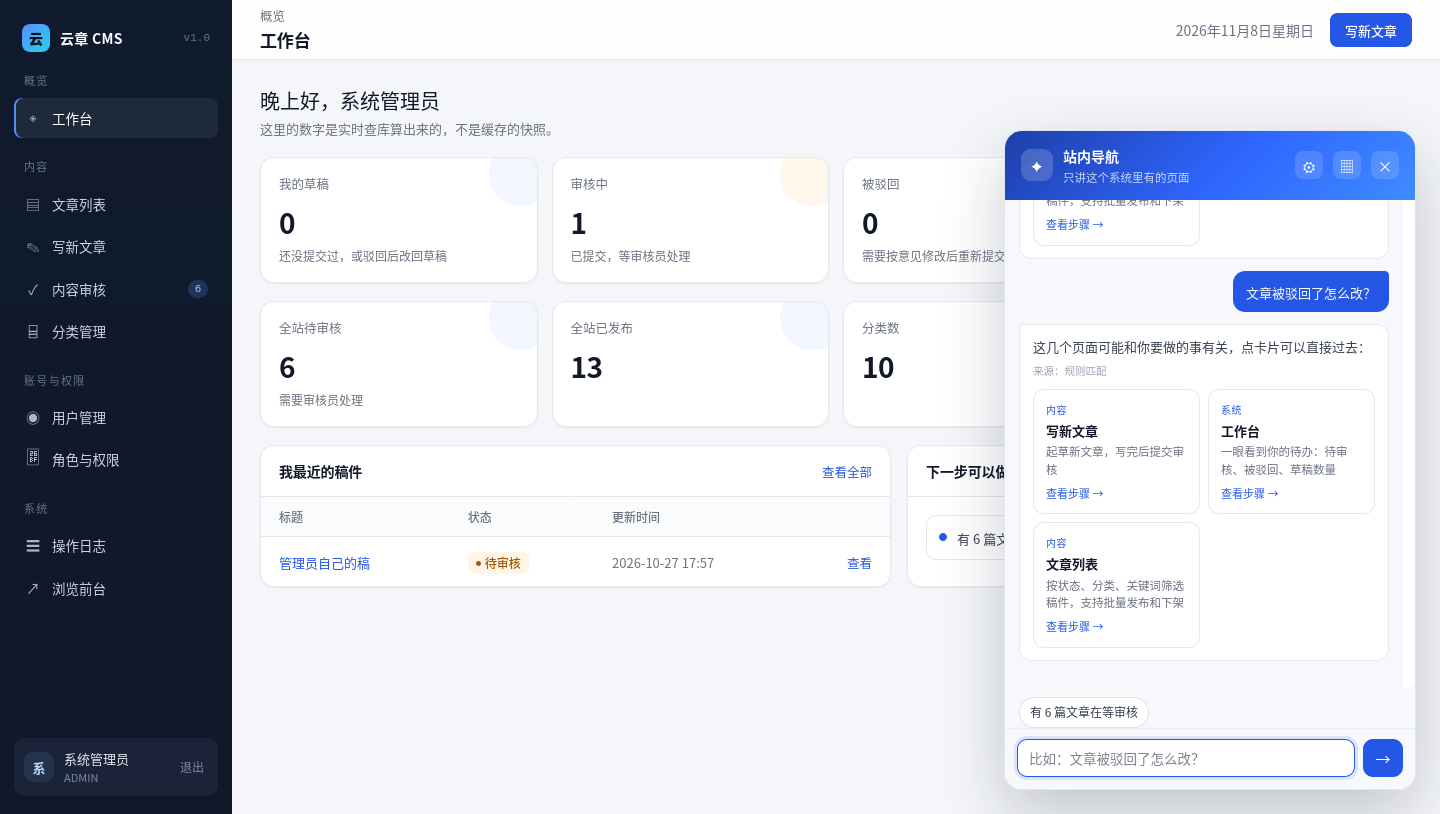
\includegraphics[width=\linewidth]{media/image15.png}

站内引导

以上截图均为 2026-11-08 在本机运行中的应用上，用无头浏览器登录 admin 后逐页实拍，不是设计稿。

\section*{九、健壮性与稳定性设计}\label{sec:robustness}
\addcontentsline{toc}{section}{九、健壮性与稳定性设计}

健壮性与稳定性不是拍脑袋保证的，它拆成三件事：先按类别把风险逐条列出来，再按等级排出处理优先级，最后用一套统一异常处理机制兜住所有出口。

\subsection*{9.1 风险分类}\label{sec:risk-class}
\addcontentsline{toc}{subsection}{9.1 风险分类}

风险按来源分成六类，逐条列出触发场景和对应业务码。

\begin{longtable}{@{}>{\raggedright\arraybackslash}p{2.9cm}>{\raggedright\arraybackslash}p{4.6cm}>{\raggedright\arraybackslash}p{4.6cm}>{\raggedright\arraybackslash}p{1.4cm}@{}}
\toprule
\textbf{风险类别} & \textbf{具体风险} & \textbf{触发场景} & \textbf{业务码} \\
\midrule
\endhead
\multicolumn{4}{@{}l}{\textbf{输入边界风险}} \\
\midrule
参数缺失 & 必填参数未传 & 40002 \\
格式非法 & 用户名、邮箱不合规 & 40000 \\
类型不匹配 & 主键 id 传成字符串 & 40000 \\
请求体不可读 & JSON 格式错误 & 40000 \\
排序字段注入 & sort 传物理列名 & 白名单拦截 \\
\midrule
\multicolumn{4}{@{}l}{\textbf{鉴权与越权风险}} \\
\midrule
未登录 & 访问受保护接口 & 40100 \\
无权限 & 角色缺对应权限点 & 40300 \\
横向越权 & 修改他人的稿件 & 40301 \\
\midrule
\multicolumn{4}{@{}l}{\textbf{状态与并发风险}} \\
\midrule
非法状态迁移 & 草稿直接发布 & 40901 \\
并发覆盖 & 两人同时改一稿 & 40900 \\
重复提交 & 并发撞唯一键 & 40902 \\
\midrule
\multicolumn{4}{@{}l}{\textbf{数据完整性风险}} \\
\midrule
删除被引用 & 删还有子分类的分类 & 40903 \\
孤儿数据 & 删用户遗留关联 & 删除前检查 \\
\midrule
\multicolumn{4}{@{}l}{\textbf{依赖与资源风险}} \\
\midrule
数据库异常 & SQL 执行失败 & 50001 \\
模型通道不可用 & 引导问答未配密钥 & 降级规则层 \\
\midrule
\multicolumn{4}{@{}l}{\textbf{信息泄漏风险}} \\
\midrule
堆栈外泄 & 未知异常 & 50000 只回通用文案 \\
敏感信息外泄 & 正文含身份证号 & 40003 硬拦加打码 \\
\bottomrule
\end{longtable}

\subsection*{9.2 风险等级与优先级}\label{sec:risk-level}
\addcontentsline{toc}{subsection}{9.2 风险等级与优先级}

按危害程度排优先级，高危先处理，低危做兜底。定级只问一句：这个风险真的发生时，损失有多大。

\begin{longtable}{@{}>{\raggedright\arraybackslash}p{1.8cm}>{\raggedright\arraybackslash}p{5.2cm}>{\raggedright\arraybackslash}p{1.6cm}>{\raggedright\arraybackslash}p{4.4cm}@{}}
\toprule
\textbf{风险等级} & \textbf{风险} & \textbf{优先级} & \textbf{定级理由} \\
\midrule
\endhead
\multicolumn{4}{@{}l}{\textbf{高危，优先处理}} \\
\midrule
高危 & 横向越权 & 1 & 数据被他人篡改，最严重 \\
高危 & 敏感信息外泄 & 2 & 隐私合规，不可逆 \\
高危 & SQL 注入 & 3 & 数据可能被拖库 \\
高危 & 堆栈外泄 & 4 & 给攻击者暴露内部结构 \\
高危 & 非法状态迁移 & 5 & 未审内容直接外发 \\
\midrule
\multicolumn{4}{@{}l}{\textbf{中危}} \\
\midrule
中危 & 并发覆盖 & 6 & 数据被互相覆盖 \\
中危 & 重复提交 & 7 & 数据重复 \\
中危 & 删除被引用 & 8 & 产生孤儿数据 \\
中危 & 未登录、无权限 & 9 & 访问失控 \\
\midrule
\multicolumn{4}{@{}l}{\textbf{低危}} \\
\midrule
低危 & 参数校验失败 & 10 & 正常拒绝，可恢复 \\
低危 & 资源不存在 & 11 & 正常分支，非故障 \\
低危 & 未知异常 & 12 & 兜底，不泄堆栈 \\
\bottomrule
\end{longtable}

\subsection*{9.3 异常处理方案设计}\label{sec:exc-design}
\addcontentsline{toc}{subsection}{9.3 异常处理方案设计}

统一异常处理由五个约定构成。

\begin{enumerate}
\item 统一 Result 壳。所有接口（含异常分支）都返回 Result，字段是 code、message、data、traceId、timestamp，前端只判断 code。
\item 错误码分段。ResultCode 用 5 位码，4xxxx 是客户端/业务错误，5xxxx 是服务端错误；HTTP 状态码表达协议层结果，code 表达业务原因，两者分离。
\item BizException 只包可预期失败。校验不过、状态非法、无权限才用它，系统异常不包，否则会把真 bug 藏起来。
\item 全局分派。GlobalExceptionHandler 用 @RestControllerAdvice 统一处理，业务异常按声明码返回，三类校验异常归并 40000，唯一键冲突归并 40902，未知异常只回 50000 通用文案。
\item traceId 全链路。MDC 注入，Result 带 traceId，sys\_log 也存 traceId，报障凭它定位这一次请求。
\end{enumerate}

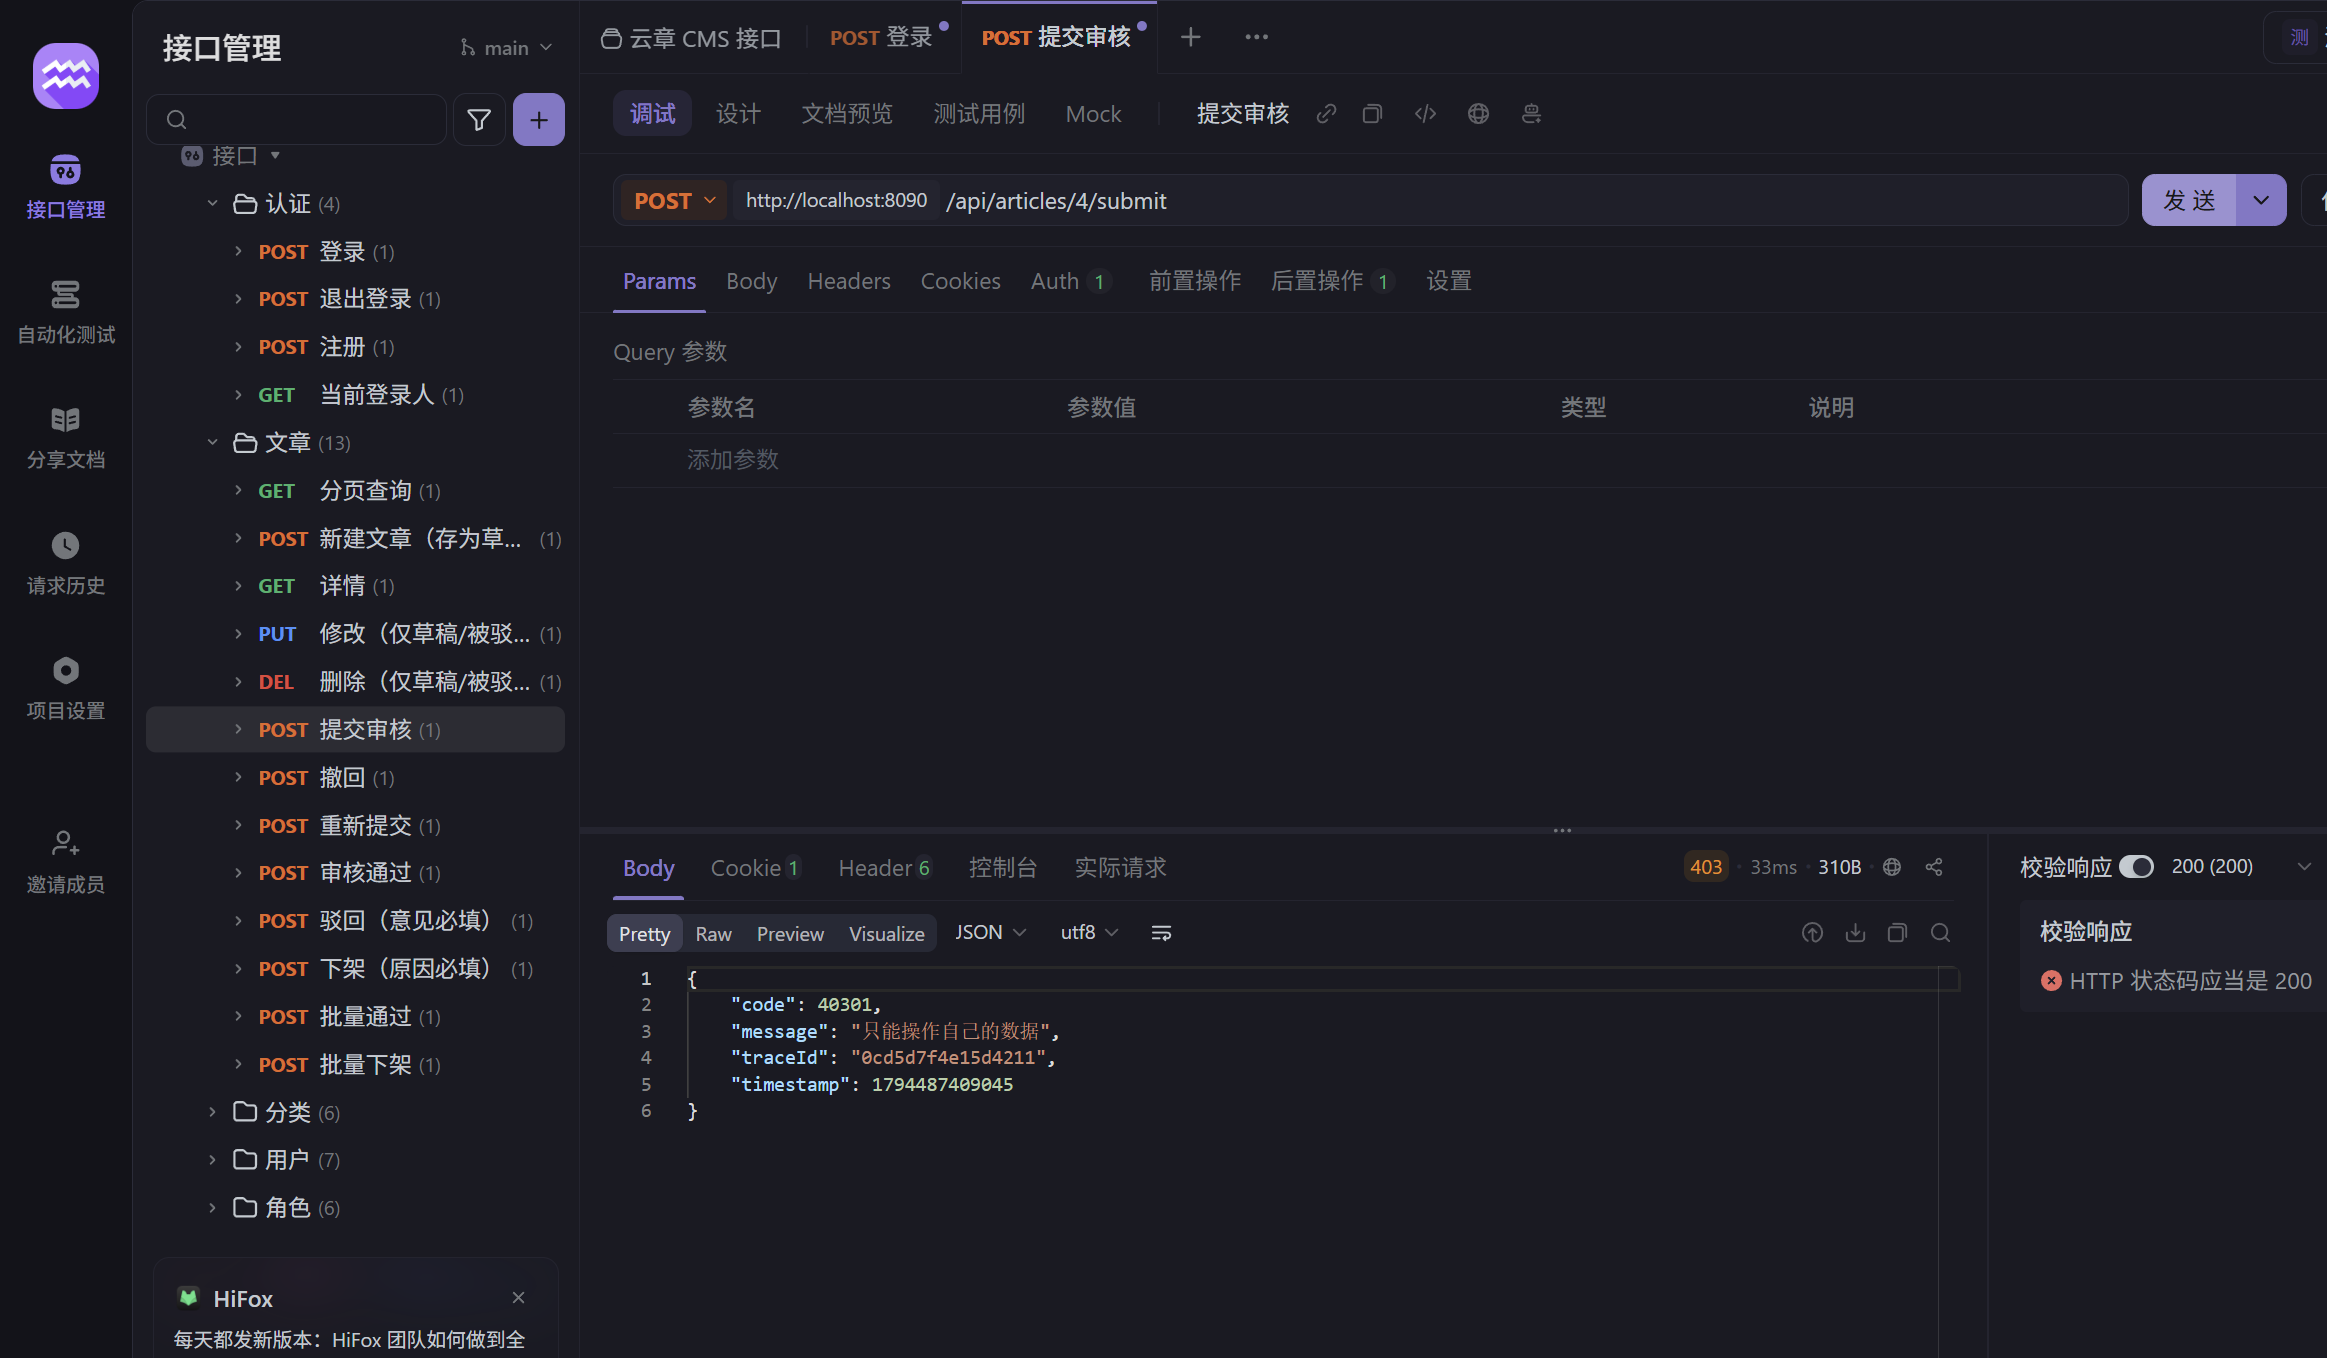
\includegraphics[width=\linewidth]{media/image53.png}

\subsection*{9.4 异常处理流程图}\label{sec:exc-flow}
\addcontentsline{toc}{subsection}{9.4 异常处理流程图}

一次请求从进入到响应，每层都有一道检查，任何一层失败都会落到统一出口。

\begin{center}
\begin{tikzpicture}[
  node distance=4mm,
  box/.style={rectangle, draw, rounded corners=1pt, align=center, minimum width=6.4cm, minimum height=0.72cm, font=\small},
  arr/.style={-{Stealth}}
]
\node[box] (a) {请求进入，LoginInterceptor 校验登录};
\node[box, below=of a] (b) {PermissionAspect 校验权限与越权};
\node[box, below=of b] (c) {Controller 接参，@Valid 校验参数};
\node[box, below=of c] (d) {Service 执行业务，失败抛 BizException};
\node[box, below=of d] (e) {GlobalExceptionHandler 按类型分派};
\node[box, below=of e] (f) {统一 Result，带业务码与 traceId};
\draw[arr] (a) -- (b);
\draw[arr] (b) -- (c);
\draw[arr] (c) -- (d);
\draw[arr] (d) -- (e);
\draw[arr] (e) -- (f);
\end{tikzpicture}
\end{center}

\subsection*{9.5 请求生命周期状态机}\label{sec:exc-state}
\addcontentsline{toc}{subsection}{9.5 请求生命周期状态机}

中间态沿主线前进，任何一步失败都进入终态。终态不可恢复，直接返回对应业务码。

\begin{center}
\begin{tikzpicture}[
  node distance=6mm and 10mm,
  state/.style={ellipse, draw, align=center, minimum width=2.6cm, minimum height=0.7cm, font=\small},
  term/.style={ellipse, draw, fill=black!10, align=center, minimum width=2.8cm, minimum height=0.75cm, font=\small},
  arr/.style={-{Stealth}}
]
\node[state] (s0) {请求到达};
\node[state, below=of s0] (s1) {登录校验};
\node[state, below=of s1] (s2) {权限校验};
\node[state, below=of s2] (s3) {参数校验};
\node[state, below=of s3] (s4) {业务处理};
\node[state, below=of s4] (s5) {成功返回 0};
\node[term, right=1.2cm of s1] (e1) {未登录 40100};
\node[term, right=1.2cm of s2] (e2) {无权限 40300\\越权 40301};
\node[term, right=1.2cm of s3] (e3) {参数错误 40000};
\node[term, right=1.2cm of s4] (e4) {业务冲突 409xx\\系统错误 50000};
\draw[arr] (s0) -- (s1);
\draw[arr] (s1) -- (s2);
\draw[arr] (s2) -- (s3);
\draw[arr] (s3) -- (s4);
\draw[arr] (s4) -- (s5);
\draw[arr] (s1) -- (e1);
\draw[arr] (s2) -- (e2);
\draw[arr] (s3) -- (e3);
\draw[arr] (s4) -- (e4);
\end{tikzpicture}
\end{center}

\subsection*{9.6 核心代码}\label{sec:exc-code}
\addcontentsline{toc}{subsection}{9.6 核心代码}

统一错误码、业务异常、全局处理器三段代码，直接取自工程。

统一错误码 ResultCode：

\begin{lstlisting}
package com.ylf.cms.common.result;

import org.springframework.http.HttpStatus;

/**
 * 统一错误码。code 采用 5 位分段：4xxxx 业务 / 客户端错误，5xxxx 服务端错误。
 * 与 HTTP 状态码分开：HTTP 状态码表达"协议层结果"，code 表达"业务原因"。
 */
public enum ResultCode {

    SUCCESS(0, "成功", HttpStatus.OK),

    BAD_REQUEST(40000, "请求参数不合法", HttpStatus.BAD_REQUEST),
    CATEGORY_LEVEL_EXCEED(40001, "分类层级超出上限（最多 3 级）", HttpStatus.BAD_REQUEST),
    PARAM_MISSING(40002, "缺少必要参数", HttpStatus.BAD_REQUEST),

    UNAUTHORIZED(40100, "未登录或登录已失效", HttpStatus.UNAUTHORIZED),
    LOGIN_FAILED(40101, "用户名或密码错误", HttpStatus.UNAUTHORIZED),
    ACCOUNT_DISABLED(40102, "账号已被停用", HttpStatus.UNAUTHORIZED),

    FORBIDDEN(40300, "没有操作权限", HttpStatus.FORBIDDEN),
    NOT_OWNER(40301, "只能操作自己的数据", HttpStatus.FORBIDDEN),

    NOT_FOUND(40400, "资源不存在", HttpStatus.NOT_FOUND),

    CONFLICT(40900, "资源状态冲突", HttpStatus.CONFLICT),
    INVALID_STATE(40901, "当前状态不允许该操作", HttpStatus.CONFLICT),
    DUPLICATE(40902, "数据已存在", HttpStatus.CONFLICT),
    IN_USE(40903, "数据被引用，无法删除", HttpStatus.CONFLICT),

    INTERNAL(50000, "系统内部错误", HttpStatus.INTERNAL_SERVER_ERROR),
    DB_ERROR(50001, "数据库操作失败", HttpStatus.INTERNAL_SERVER_ERROR);

    private final int code;
    private final String message;
    private final HttpStatus status;

    ResultCode(int code, String message, HttpStatus status) {
        this.code = code;
        this.message = message;
        this.status = status;
    }

    public int getCode() {
        return code;
    }

    public String getMessage() {
        return message;
    }

    public HttpStatus getStatus() {
        return status;
    }
}
\end{lstlisting}

业务异常 BizException：

\begin{lstlisting}
package com.ylf.cms.common.exception;

import com.ylf.cms.common.result.ResultCode;

/**
 * 业务异常。只用于"可预期的失败"（校验不过、状态非法、无权限），
 * 不用于包装系统异常——那样会把真正的 bug 藏起来。
 */
public class BizException extends RuntimeException {

    private final ResultCode resultCode;

    public BizException(ResultCode resultCode) {
        super(resultCode.getMessage());
        this.resultCode = resultCode;
    }

    public BizException(ResultCode resultCode, String message) {
        super(message);
        this.resultCode = resultCode;
    }

    public ResultCode getResultCode() {
        return resultCode;
    }
}
\end{lstlisting}

全局异常处理器 GlobalExceptionHandler：

\begin{lstlisting}
package com.ylf.cms.common.exception;

import com.ylf.cms.common.result.Result;
import com.ylf.cms.common.result.ResultCode;
import lombok.extern.slf4j.Slf4j;
import org.springframework.dao.DuplicateKeyException;
import org.springframework.http.ResponseEntity;
import org.springframework.http.converter.HttpMessageNotReadableException;
import org.springframework.validation.BindException;
import org.springframework.validation.FieldError;
import org.springframework.web.HttpRequestMethodNotSupportedException;
import org.springframework.web.bind.MethodArgumentNotValidException;
import org.springframework.web.bind.MissingServletRequestParameterException;
import org.springframework.web.bind.annotation.ExceptionHandler;
import org.springframework.web.bind.annotation.RestControllerAdvice;
import org.springframework.web.method.annotation.MethodArgumentTypeMismatchException;

import javax.validation.ConstraintViolation;
import javax.validation.ConstraintViolationException;
import java.util.stream.Collectors;

/**
 * 全局异常处理。
 *
 * 三条原则：
 * 1. 业务异常按声明的错误码返回，HTTP 状态码与 code 各自表达不同层次；
 * 2. 未知异常只回"系统内部错误"，堆栈只进服务端日志——把堆栈回给前端等于免费送攻击面；
 * 3. 每个响应带 traceId，用户报障时凭它能在日志里定位到这一次请求。
 */
@Slf4j
@RestControllerAdvice
public class GlobalExceptionHandler {

    @ExceptionHandler(BizException.class)
    public ResponseEntity<Result<Void>> handleBiz(BizException e) {
        ResultCode rc = e.getResultCode();
        return ResponseEntity.status(rc.getStatus())
                .body(Result.fail(rc, e.getMessage()));
    }

    @ExceptionHandler(MethodArgumentNotValidException.class)
    public ResponseEntity<Result<Void>> handleValid(MethodArgumentNotValidException e) {
        String msg = e.getBindingResult().getFieldErrors().stream()
                .map(this::describe)
                .collect(Collectors.joining("；"));
        return badRequest(msg);
    }

    @ExceptionHandler(BindException.class)
    public ResponseEntity<Result<Void>> handleBind(BindException e) {
        String msg = e.getBindingResult().getFieldErrors().stream()
                .map(this::describe)
                .collect(Collectors.joining("；"));
        return badRequest(msg);
    }

    @ExceptionHandler(ConstraintViolationException.class)
    public ResponseEntity<Result<Void>> handleConstraint(ConstraintViolationException e) {
        String msg = e.getConstraintViolations().stream()
                .map(ConstraintViolation::getMessage)
                .collect(Collectors.joining("；"));
        return badRequest(msg);
    }

    @ExceptionHandler(MissingServletRequestParameterException.class)
    public ResponseEntity<Result<Void>> handleMissingParam(MissingServletRequestParameterException e) {
        return ResponseEntity.status(ResultCode.PARAM_MISSING.getStatus())
                .body(Result.fail(ResultCode.PARAM_MISSING, "缺少参数：" + e.getParameterName()));
    }

    @ExceptionHandler(MethodArgumentTypeMismatchException.class)
    public ResponseEntity<Result<Void>> handleTypeMismatch(MethodArgumentTypeMismatchException e) {
        return badRequest("参数类型不正确：" + e.getName());
    }

    @ExceptionHandler(HttpMessageNotReadableException.class)
    public ResponseEntity<Result<Void>> handleUnreadable(HttpMessageNotReadableException e) {
        return badRequest("请求体格式不正确");
    }

    @ExceptionHandler(HttpRequestMethodNotSupportedException.class)
    public ResponseEntity<Result<Void>> handleMethod(HttpRequestMethodNotSupportedException e) {
        return ResponseEntity.status(ResultCode.BAD_REQUEST.getStatus())
                .body(Result.fail(ResultCode.BAD_REQUEST, "不支持的请求方法：" + e.getMethod()));
    }

    @ExceptionHandler(DuplicateKeyException.class)
    public ResponseEntity<Result<Void>> handleDuplicate(DuplicateKeyException e) {
        // 唯一索引兜底：并发下先查后插仍可能撞车，靠数据库约束给出可读错误
        log.warn("唯一约束冲突: {}", e.getMostSpecificCause().getMessage());
        return ResponseEntity.status(ResultCode.DUPLICATE.getStatus())
                .body(Result.fail(ResultCode.DUPLICATE));
    }

    @ExceptionHandler(Exception.class)
    public ResponseEntity<Result<Void>> handleOther(Exception e) {
        log.error("未捕获异常", e);
        return ResponseEntity.status(ResultCode.INTERNAL.getStatus())
                .body(Result.fail(ResultCode.INTERNAL));
    }

    private ResponseEntity<Result<Void>> badRequest(String message) {
        return ResponseEntity.status(ResultCode.BAD_REQUEST.getStatus())
                .body(Result.fail(ResultCode.BAD_REQUEST, message));
    }

    private String describe(FieldError fe) {
        return fe.getField() + " " + fe.getDefaultMessage();
    }
}
\end{lstlisting}

\section*{十、重难点与解决方案}\label{ux516bux91cdux96beux70b9ux4e0eux89e3ux51b3ux65b9ux6848}
\addcontentsline{toc}{section}{十、重难点与解决方案}



\subsection*{10.1 状态机写成表，而不是散落的 if}\label{ux72b6ux6001ux673aux5199ux6210ux8868ux800cux4e0dux662fux6563ux843dux7684-if}
\addcontentsline{toc}{subsection}{10.1 状态机写成表，而不是散落的 if}

难点在于文章状态在多个接口里被修改，每处都写 if (status == X)，新增一条迁移要改多处，也很难证明没有非法路径。

做法是把当前状态加动作到下一状态的映射存成静态表，未命中就抛 INVALID\_STATE。单测逐条断言 7 条合法边、4 组非法组合以及删除规则，非法组合包括草稿直接通过、已发布直接改、已下架再下架、被驳回直接提交。

收益是状态图与代码成为同一份事实，改代码就必须改图。

\subsection*{10.2 横向越权：接口权限无法阻止修改他人数据}\label{ux6a2aux5411ux8d8aux6743ux63a5ux53e3ux6743ux9650ux7ba1ux4e0dux4f4fux6539ux522bux4ebaux7684ux6570ux636e}
\addcontentsline{toc}{subsection}{10.2 横向越权：接口权限无法阻止修改他人数据}

难点在于 author 有 article:update:own 权限，AOP 看到权限码就放行，但接口 /api/articles/\{id\} 的 id 可以是别人的稿子。

做法是 AOP 只做第一层，Service 里 checkOwner 做第二层，:any 直接过，:own 必须比对 authorId。用 bob 的草稿 id 实测，以 alice 身份请求，返回 403/40301。

\subsection*{10.3 列表页的 N+1}\label{ux5217ux8868ux9875ux7684-n1}
\addcontentsline{toc}{subsection}{10.3 列表页的 N+1}

见 8.3。判据是 mapper DEBUG 日志的 SQL 条数，不是主观感受。

\subsection*{10.4 模块边界：文档约束必须有判据}\label{ux6a21ux5757ux8fb9ux754cux8fd9ux79cdux6587ux6863ux91ccux7684ux4e00ux53e5ux8bddux5fc5ux987bux6709ux5224ux636e}
\addcontentsline{toc}{subsection}{10.4 模块边界：文档约束必须有判据}

见 6.3。核心教训是测试绿不等于代码对，可能只是判据没有覆盖到真正的越界，必须主动注入越界代码验证它会变红。

\subsection*{10.5 智能体不得编造不存在的功能}\label{ux667aux80fdux4f53ux4e0dux80fdux7b54ux4e0dux51faux5c31ux7f16}
\addcontentsline{toc}{subsection}{10.5 智能体不得编造不存在的功能}

难点在于让模型自由回答，它一定会编出站点里不存在的页面。

做法是把模型能说什么收缩成封闭集合。启动期生成 9 张卡片，模型只能在里面选 id，越界就丢弃。规则层未命中且模型不可用时就明说系统里没有这个功能，不强行返回卡片。

\subsection*{10.6 敏感信息的误判与日志二次泄漏}\label{ux654fux611fux4fe1ux606fux7684ux8befux5224ux4e0eux65e5ux5fd7ux4e8cux6b21ux6cc4ux6f0f}
\addcontentsline{toc}{subsection}{10.6 敏感信息的误判与日志二次泄漏}

第一个难点是见数字就拦，会让订单号、统计数字全被误伤，用户很快学会无视提示框。做法是身份证走 GB 11643 校验位，银行卡走 Luhn，18 位数字本身不算命中。同一片段做区间占位，防止 18 位身份证碰巧通过 Luhn 后被同时报成银行卡。

第二个难点是拦住了提交，但被拒绝的请求参数仍会进 sys\_log。做法是日志写入前用同一套规则打码，判据是日志表里搜不到原文。

\subsection*{10.7 问题与方案汇总}\label{ux95eeux9898ux4e0eux65b9ux6848ux6c47ux603b}
\addcontentsline{toc}{subsection}{10.7 问题与方案汇总}

非法状态迁移靠显式状态表加 40901 解决，由 ArticleStateMachineTest 逐条断言。并发覆盖靠 @Version 乐观锁解决，并发修改返回 40900。横向越权靠 AOP 加 checkOwner 双层解决，越权返回 40301。N+1 靠三表 join 加分页插件解决，mapper DEBUG 日志只剩 2 条 SQL。排序注入靠逻辑名到物理列的白名单解决，非法 sort 返回 40000。全表更新靠 BlockAttackInnerInterceptor 解决，没有 where 的 update 被拦截。删除孤儿数据靠删除前计数解决，返回 40903。模块越界引用靠 import 扫描测试解决，注入越界 import 后测试变红。引导答非所问靠封闭卡片集合加阈值解决，越界 cardId 被丢弃。敏感信息外泄靠预检、硬拦加日志打码解决，对应 40003、弹窗与日志检查。堆栈外泄靠统一异常处理只回通用文案解决，未知异常返回 50000。

\section*{十一、AI 辅助·人脑主导}\label{ux4e5dai-ux8f85ux52a9ux4ebaux8111ux4e3bux5bfc}
\addcontentsline{toc}{section}{十一、AI 辅助·人脑主导}



\subsection*{11.1 分工原则}\label{ux5206ux5de5ux539fux5219}
\addcontentsline{toc}{subsection}{11.1 分工原则}

AI 负责生成脚手架，包括 pom、配置、目录，以及重复度高的 CRUD 片段和接口文档骨架；本人逐行校验，涉及状态、权限、事务、并发的地方自行设计与改写。AI 提供 MP 插件顺序、Spring AOP 写法等模板；本人排查分页失效但无报错这类静默失败。AI 解释报错、给出候选方案；本人决定取舍，例如坚决不引入整套 Spring Security。

原则可以概括为一句话。AI 负责我知道它大概怎么写，本人负责我知道它为什么对。凡是需要判断这段代码在什么情况下会错的地方，都不接受 AI 的直接产出。

\subsection*{11.2 过程痕迹}\label{ux8fc7ux7a0bux75d5ux8ff9}
\addcontentsline{toc}{subsection}{11.2 过程痕迹}

docs/ai-log.md 按天记录当天做了什么、AI 给了什么建议、人工发现了什么错、做了哪些验证。调试记录与代码修改痕迹保留在仓库中。

\subsection*{11.3 三个由人发现而 AI 未看出的实例}\label{ux4e09ux4e2aux4ebaux8111ux53d1ux73b0-ai-ux6ca1ux770bux51faux7684ux5b9eux4f8b}
\addcontentsline{toc}{subsection}{11.3 三个由人发现而 AI 未看出的实例}

第一个实例是模块边界测试第一次出现假通过，见 6.3。AI 写的判据把包位置写死在 import 的第二段，运行时路径却在第三段，测试对越界代码照样放行，靠人工注入才发现。

第二个实例是迁移重命名后，测试报告出现两份同名结果。旧 class 文件还留在 target/classes 里被扫描，删源码不等于删 Bean，必须 mvn clean。这类问题 AI 不会主动提醒，因为当前代码是对的。

第三个实例是日志脱敏第一版按类名前缀判断，漏掉了容器注入的 RequestFacade，真实请求日志里那串 org.apache.catalina...@28ef8fa8 才暴露出来。正确做法是判断 instanceof ServletRequest，而不是猜类名。

\subsection*{11.4 不把 AI 的产出当结论}\label{ux4e0dux628a-ai-ux7684ux4ea7ux51faux5f53ux7ed3ux8bba}
\addcontentsline{toc}{subsection}{11.4 不把 AI 的产出当结论}

文档与代码对账过一轮，删掉了文档里有而代码里没有的描述，比如 Session 写成 token、登录锁定、多轮上下文等。反过来，逻辑删除造成的孤儿数据这类真实缺陷，补的是代码而不是改文档。本次编写报告时又发现一处，接口文档原写注册默认 GUEST 角色，实际代码是 RoleCode.DEFAULT = AUTHOR，已按代码订正。

性能结论来自 SQL 条数，不来自应该会更快的主观判断。

卡片清单来自启动期反射，不来自手写清单。

\subsection*{11.5 AI 优化总结}\label{ai-ux4f18ux5316ux603bux7ed3}
\addcontentsline{toc}{subsection}{11.5 AI 优化总结}

AI 在本项目中的正确定位是放大器而非替代品，具体体现在三类用法。

第一类是生成再到校验。脚手架与模板由 AI 生成，但每一条都要能回答它在什么输入下会错。校验的成本远低于从零手写的成本，这正是收益所在。

第二类是排错再到归因。AI 擅长根据报错给出候选原因，但哪个原因成立必须用可执行判据验证，比如注入、日志、SQL 条数，不接受应该就是这个原因。

第三类是重构再到收敛。AI 建议的抽象，例如把状态判断抽成表，先做小范围验证，确认判据能覆盖全部边再推广。

反过来，有三类事情不适合交给 AI 直接产出，涉及并发与事务的正确性判断、安全边界的取舍、以及任何看起来对但没有判据的结论。本项目中这三类问题全部由人工设计与验证，AI 只参与讨论与提供候选方案。

\section*{十二、编码规范与工程质量}\label{ux5341ux7f16ux7801ux89c4ux8303ux4e0eux5de5ux7a0bux8d28ux91cf}
\addcontentsline{toc}{section}{十二、编码规范与工程质量}



\subsection*{12.1 命名规范}\label{ux547dux540dux89c4ux8303}
\addcontentsline{toc}{subsection}{12.1 命名规范}

包名全小写，按业务域划分，例如 com.ylf.cms.content.service。类名大驼峰，后缀表意，例如 ArticleStateMachine、SensitiveInfoDetector。方法名动词开头、小驼峰，例如 checkOwner、batchApprove、maskAll。常量全大写下划线，例如 Perm.ARTICLE\_AUDIT、RoleCode.DEFAULT。数据库表名用 snake\_case 带域前缀，列名也 snake\_case，例如 cms\_article、audit\_opinion。索引与外键用 uk\_、idx\_、fk\_ 前缀加表简称加语义，例如 uk\_category\_parent\_name。

\subsection*{12.2 注释规范}\label{ux6ce8ux91caux89c4ux8303}
\addcontentsline{toc}{subsection}{12.2 注释规范}

注释只写为什么，不写是什么。三类地方必须有注释。

第一类是不显然的取舍，例如用户名不可改，因为日志靠它做可读追溯。

第二类是容易踩的坑，例如插件顺序错了会出现分页失效却无报错。

第三类是反直觉的实现，例如 parent\_id 取 0 而非 NULL，因为 NULL 不参与唯一索引去重。

类注释说明职责与边界；公共方法注释说明参数含义与异常条件。没有注释的代码应当做到"看名字就知道在做什么"。

\subsection*{12.3 分层与职责单一}\label{ux5206ux5c42ux4e0eux804cux8d23ux5355ux4e00}
\addcontentsline{toc}{subsection}{12.3 分层与职责单一}

Controller 主要负责：接参、校验、调 Service、包装返回值，不写业务判断。Service 承担业务规则与事务边界。Mapper 只做数据访问，复杂 SQL 放 XML。DTO 与 VO 分离：入参用 DTO，出参用 VO，实体不直接暴露给接口。

\subsection*{12.4 健壮性与稳定性}\label{ux5065ux58eeux6027ux4e0eux7a33ux5b9aux6027}
\addcontentsline{toc}{subsection}{12.4 健壮性与稳定性}

参数边界用 @Valid 加注解校验，排序字段走白名单，分页上限 200。数据完整性靠真实外键、删除前引用检查与逻辑删除。并发靠乐观锁，唯一索引兜底重复提交。异常走统一处理器，业务码与 HTTP 码分离，未知异常不泄堆栈。会话设置 30 分钟超时，Cookie 加 httpOnly 与 sameSite=lax。安全靠 BCrypt、敏感信息三层防护与 \#\{\} 预编译。

\section*{十三、测试与验证}\label{ux5341ux4e00ux6d4bux8bd5ux4e0eux9a8cux8bc1}
\addcontentsline{toc}{section}{十三、测试与验证}



\subsection*{13.1 单元测试}\label{ux5355ux5143ux6d4bux8bd5}
\addcontentsline{toc}{subsection}{13.1 单元测试}

mvn -o test 共 33 个用例，分属 6 个测试类，全部通过。

ArticleStateMachineTest 有 4 个用例，覆盖 7 条合法边、非法组合、各状态可用动作与删除规则。SensitiveInfoDetectorTest 有 9 个用例，覆盖六类敏感信息、校验位误判、区间占位与日志打码。SiteMapValidatorTest 有 8 个用例，覆盖 C1--C5 五条校验及组合。IntentRouterTest 有 5 个用例，覆盖规则层命中、未命中、多意图与空输入。GuideLlmServiceTest 有 5 个用例，覆盖密钥存取、只回尾号、开关关闭时忽略与连接测试失败路径。ModuleBoundaryTest 有 2 个用例，扫描跨模块越界引用。

\subsection*{13.2 实机联调}\label{ux5b9eux673aux8054ux8c03}
\addcontentsline{toc}{subsection}{13.2 实机联调}

四个账号（admin / author / auditor / guest）全链路联调通过，覆盖：注册 → 登录 → 建稿 → 提交 → 审核 → 发布 → 下架 → 再提交；分类增删改停；用户与角色分配；日志查询；前台阅读。

\subsection*{13.3 接口异常矩阵}\label{ux63a5ux53e3ux5f02ux5e38ux77e9ux9635}
\addcontentsline{toc}{subsection}{13.3 接口异常矩阵}

未登录访问受保护接口返回 401 与 40100。无权限角色调用返回 403 与 40300。作者改他人稿件返回 403 与 40301。访问不存在的文章返回 404 与 40400。非法状态迁移返回 409 与 40901。删除被引用的分类返回 409 与 40903。正文含敏感信息返回 400 与 40003。未知异常返回 500 与 50000。以上均实测通过。

所有响应均带 traceId，可与 sys\_log 对应。

\subsection*{13.4 浏览器实测}\label{ux6d4fux89c8ux5668ux5b9eux6d4b}
\addcontentsline{toc}{subsection}{13.4 浏览器实测}

写稿页敏感信息提示框用 Selenium + 无头 Firefox 实测，8 项断言全部通过（输入 → 预检接口返回 → 弹窗出现 → 阻止提交 → 日志打码）。

\subsection*{13.5 已知边界与未实测项}\label{ux5df2ux77e5ux8fb9ux754cux4e0eux672aux5b9eux6d4bux9879}
\addcontentsline{toc}{subsection}{13.5 已知边界与未实测项}

以下各项如实列出，不假装支持。

测试覆盖偏结构性。33 个用例集中在状态机、边界扫描、检测器与引导校验，Service 层的数据库交互仍靠实机联调，未引入 H2 或 Testcontainers 做集成测试，因此单测全绿不等于 SQL 全对。

性能未做压测。N+1 优化有 SQL 条数判据，但没有并发压测数据。全文检索用 LIKE \%kw\%，十万级数据后需要走索引或换搜索引擎，EXPLAIN 对照已写进演示脚本，但未做基准测试。

并发正确性只做功能验证。乐观锁的冲突路径有用例，但没有做多线程压力测试来验证确实只有一个成功。

引导的长问句依赖模型通道。规则层对多卡片意图的处理是都返回让用户挑，体验一般。

前端无构建链。代码复用靠约定，页面再多会失控，属于刻意取舍。

\section*{十四、部署与交付}\label{ux5341ux4e8cux90e8ux7f72ux4e0eux4ea4ux4ed8}
\addcontentsline{toc}{section}{十四、部署与交付}



\subsection*{14.1 环境要求}\label{ux73afux5883ux8981ux6c42}
\addcontentsline{toc}{subsection}{14.1 环境要求}

JDK 版本 11。Maven 3.6 以上，依赖已缓存时可加 -o 离线构建。数据库用 MySQL 8 或 MariaDB 10.6 以上，本项目联调使用 MariaDB 10.6.23。服务端口 8090，因为本机 8080 被系统级 tomcat9 占用。

\subsection*{14.2 三步启动}\label{ux4e09ux6b65ux542fux52a8}
\addcontentsline{toc}{subsection}{14.2 三步启动}

\# 1. 建库（创建 cms\_db 与 cmsapp 账号并导入 schema / data）\\
sudo bash db/init.sh\\
\strut \\
\# 2. 启动\\
mvn spring-boot:run\\
\strut \\
\# 3. 打开 http://localhost:8090 ，用 admin / 123456 登录

停止服务：pkill -f spring-boot:run。

\subsection*{14.3 演示账号}\label{ux6f14ux793aux8d26ux53f7}
\addcontentsline{toc}{subsection}{14.3 演示账号}

演示账号共四个，密码均为 123456。admin 对应 ADMIN 角色，author 对应 AUTHOR，auditor 对应 AUDITOR，guest 对应 GUEST。

\subsection*{14.4 交付物清单}\label{ux4ea4ux4ed8ux7269ux6e05ux5355}
\addcontentsline{toc}{subsection}{14.4 交付物清单}

cms-project/\\
|- pom.xml 依赖与构建\\
|- README.md 功能清单、三步启动、演示账号、已知边界\\
|- db/init.sh 一键建库脚本\\
|- apifox/cms-openapi.json OpenAPI 3.0，可直接导入 Apifox\\
|- src/main/\\
| |- java/com/ylf/cms/ 103 个 Java 文件（6 个业务/公共包）\\
| `- resources/\\
| |- sql/\{schema.sql,data.sql\} 建表与初始化数据\\
| |- mapper/ArticleMapper.xml 多表 join 与动态条件\\
| |- guide/site-map.yaml 引导站点地图（受启动期校验）\\
| |- templates/ 13 个 Thymeleaf 模板\\
| `- static/ 17 个前端模块\\
|- src/test/java/ 33 个单元测试\\
`- docs/\\
|- 课程设计报告.md / .docx / .pdf 本文\\
|- 需求分析.md 七场景、权限矩阵、跟踪矩阵\\
|- 表结构说明.md 8 张表逐字段说明\\
|- api.md 49 个操作的请求/响应示例\\
|- 测试记录.md 单测 / 实机联调 / 修掉的缺陷\\
|- ai-log.md AI 交互与人工校验记录\\
|- 实验总结.md 分工、问题、收获、不足\\
|- 演示脚本.md 十幕演示流程\\
|- 任务书.md / 分工说明.md\\
|- diagrams/ 架构 / E-R / 流程 / 状态机 / 时序\\
`- screenshots/ 10 张界面实拍

\section*{十五、总结与不足}\label{ux5341ux4e09ux603bux7ed3ux4e0eux4e0dux8db3}
\addcontentsline{toc}{section}{十五、总结与不足}



\subsection*{做得好的方面}\label{ux505aux5bf9ux4e86ux4ec0ux4e48}
\addcontentsline{toc}{subsection}{做得好的方面}

第一，约束用测试表达，不用文档表达。模块边界、状态迁移、启动期卡片校验都有可执行判据。文档会腐烂，测试不会。

第二，失败路径与成功路径同等重要。非法迁移、越权、并发冲突、敏感内容、模型越界，每一条都有明确错误码与实测记录。

第三，不假装能力。没有上传功能就不写上传，没有压测数据就说没有压测，文档与代码对过账。

第四，复杂规则集中成表。状态机、权限码、错误码、排序白名单都是集中定义、多处引用的表，避免同一规则在多处各写一遍。

\subsection*{不足之处}\label{ux8fd8ux9700ux8981ux6539ux8fdbux4ec0ux4e48}
\addcontentsline{toc}{subsection}{不足之处}

第一，补充集成测试。用 Testcontainers 拉起真实 MySQL，覆盖 Service 层的 SQL 正确性，弥补单测不碰数据库的空档。

第二，补充并发与性能基准。对乐观锁做多线程验证，对列表查询做 EXPLAIN 与不同数据量下的耗时对比。

第三，补强检索能力。LIKE 在前缀匹配下可用，模糊匹配到一定数据量必然退化，需要引入倒排索引或搜索引擎。

第四，推进前端工程化。当前无构建链是刻意取舍，但如果页面继续增加，模块化与复用会成为瓶颈。

\subsection*{收获}\label{ux6536ux83b7}
\addcontentsline{toc}{subsection}{收获}

这次设计最大的收获不是写完了多少功能，而是学会了如何证明一个东西是对的。判据要能被否证，测试要能被注入弄红，性能要有日志条数，文档要与代码对账，模型输出要能越界被丢弃。一条无法失败的判据，和没有判据是一样的。

\section*{附录 A：AI 合理应用与代码优化}\label{app-ai-rational}
\addcontentsline{toc}{section}{附录 A：AI 合理应用与代码优化}

本附录对应评分标准第五项“AI 合理应用与代码优化”，满分 2 分，拆成两个评分点：AI 辅助·人脑主导占 1 分，过程痕迹占 1 分。正文第十一章已经讲过分工原则和三个反例，这里按评分点逐条展开，把 AI 到底做了什么、本人独立完成了什么、留下了哪些痕迹，一一说清楚。

\subsection*{A.1 AI 辅助·人脑主导（1 分）}\label{app-ai-human-led}
\addcontentsline{toc}{subsection}{A.1 AI 辅助·人脑主导（1 分）}

AI 在本项目里的使用边界只有三类，每一类都配逐行人工校验；超出这三类的四类工作，全部由本人独立完成，AI 不参与直接产出。

先说 AI 负责的三类。

第一类，基础配置。AI 生成 pom.xml 的依赖清单、application.yml 的配置项和工程目录骨架。本人逐行核对依赖版本与 JDK 11、Spring Boot 2.7.18、MyBatis-Plus 3.5.3.1 的兼容性，确认没有引入多余依赖，配置项与代码里的实际取值一致。配置写错了不会在编译期报错，只会在运行期炸，所以这类看似简单的活也必须逐行看。

第二类，通用片段。AI 生成 entity、mapper、service、controller 的 CRUD 重复骨架。本人逐行核对字段映射、@TableName 与 @TableId 注解、逻辑删除 deleted 字段与审计四字段的自动填充，保证骨架和真实表结构对齐。骨架的价值是省掉重复打字，但字段多一个少一个、注解错一个，运行期就会静默出错，省下的时间不能以漏核对为代价。

第三类，接口模板。AI 生成 Controller 方法签名与 OpenAPI 文档骨架。本人逐行核对返回结构、五位业务码、@RequirePermission 权限注解，保证文档和实现一致。接口是安全边界，权限注解错一个就是越权，这一行必须人来把关。

再说本人独立完成的四类。

复杂逻辑，本人设计与实现，包括文章状态机、权限判定链、分类树循环检测、敏感信息识别。这些地方一旦逻辑错，不会有报错提示，只会悄悄放行或拦截，所以不交给 AI 直接产出。

排错，本人定位并修复，包括分页失效但无报错的静默失败、日志脱敏漏掉容器注入的 RequestFacade、模块边界测试假通过。排错的关键是归因，AI 只能给候选原因，哪个成立必须本人用可执行判据验证。

优化，本人给出方案并验证，包括把列表页从 1+N 条 SQL 降到 2 条的三表 join、索引设计、排序白名单。优化的判据是能数出来的数字，不是“应该会更快”的主观感觉。

重构，本人先小范围验证再推广，包括把状态判断抽成表、错误码集中定义、公共逻辑抽取。重构的风险在于改坏了没有判据能发现，所以先验证、再收敛。

判断标准只有一句话：凡是需要回答这段代码在什么情况下会错的地方，都不接受 AI 的直接产出。AI 负责“我知道它大概怎么写”，本人负责“我知道它为什么对”。

\subsection*{A.2 过程痕迹（1 分）}\label{app-ai-traces}
\addcontentsline{toc}{subsection}{A.2 过程痕迹（1 分）}

过程痕迹分三类，全部保留在仓库里，可以随时翻出来对照，用于证明自主开发过程。

第一类，AI 交互记录。docs/ai-log.md 按天记录当天做了什么、AI 给了什么建议、人工发现了什么错、做了哪些验证。每一条建议都注明了采纳还是拒绝，拒绝的都写了原因，不是只留结果不留判断。

第二类，代码修改痕迹。本地 git 仓库保留完整提交历史，每一次提交对应一个明确的功能或修复，提交信息写清楚改了什么、为什么改。从初始脚手架到最后成品的每一步都能回溯。

第三类，调试与验证记录。mapper DEBUG 日志保留在文档里，能数出优化前后的 SQL 条数；测试注入记录保留在模块边界测试里；越权请求的返回体保留在截图里。这些不是事后补写的，而是开发当时留下的现场。

三类痕迹合在一起，能完整还原从脚手架到成品的开发过程：哪一步是 AI 生成的、哪一步是本人改的、哪一步是本人从零写的，都有据可查，体现自主开发过程。

\subsection*{A.3 代码优化对照}\label{app-ai-opt}
\addcontentsline{toc}{subsection}{A.3 代码优化对照}

“代码优化”是第五项评分里与 AI 并列的另一半，下面是本项目主要优化点与判据的对照。

\begin{longtable}{@{}>{\raggedright\arraybackslash}p{3.2cm}>{\raggedright\arraybackslash}p{6.2cm}>{\raggedright\arraybackslash}p{3.4cm}@{}}
\toprule
\textbf{优化点} & \textbf{做法} & \textbf{判据} \\
\midrule
\endfirsthead
\multicolumn{3}{@{}l}{\small（续表）}\\
\toprule
\textbf{优化点} & \textbf{做法} & \textbf{判据} \\
\midrule
\endhead
列表页 N+1 & 三表 join 一次带出分类与作者 & SQL 从 41 条降到 2 条 \\
排序注入 & 白名单映射物理列，非法字段抛错 & 非法字段返回 40000 \\
全表误更新 & BlockAttack 拦截无 where 的 update/delete & 缺 where 直接报错 \\
并发覆盖 & 乐观锁 @Version，冲突不静默覆盖 & 冲突返回 40900 \\
逻辑删除 & deleted 字段加 @TableLogic 全局过滤 & 删除后可恢复 \\
审计字段 & MetaObjectHandler 自动填充四字段 & 业务代码不手写 \\
\bottomrule
\end{longtable}

每一行的判据都不是“看起来优化了”，而是能数出来、能测出来、能复现的指标，这与 A.1 里“凡是没有判据的结论都不接受”是同一套原则。

\end{document}
